% Plantilla de trabajo: confirmar normas vigentes de tesis UDLAP antes de fijarla.
\documentclass[12pt,letterpaper,oneside]{report}
% Toda elección de formato es provisional hasta confirmar las normas UDLAP.
\usepackage[T1]{fontenc}
\usepackage{iftex}
\ifPDFTeX\usepackage[utf8]{inputenc}\fi
\usepackage[spanish,es-nodecimaldot,es-tabla]{babel}
\usepackage{lmodern}
\usepackage[margin=2.5cm]{geometry}
\usepackage{setspace}
\onehalfspacing
\usepackage{amsmath,amssymb}
\usepackage{booktabs,array,longtable}
\usepackage{graphicx}
\usepackage{caption}
\captionsetup{font=small,labelfont=bf}
\usepackage[authoryear,round]{natbib}
\usepackage{xurl}
\usepackage[unicode,hidelinks]{hyperref}
\hypersetup{pdftitle={Borrador de tesis: vulnerabilidad económica longitudinal en ENASEM},
            pdfauthor={Andrea}, pdfsubject={CP1; revisión metodológica pendiente}}
\newcommand{\doi}[1]{\href{https://doi.org/#1}{DOI: \nolinkurl{#1}}}
\setlength{\parindent}{1.2em}
\setlength{\parskip}{0.2em}
\setlength{\emergencystretch}{2em}
\newcommand{\variable}[1]{\nolinkurl{#1}}
\newcommand{\estadoBorrador}{\textit{Borrador: pendiente de revisión académica.}}
% Referencia visual: cuadros 3.1--3.5 del borrador original de la autora.
% Confirmar todavía las normas institucionales UDLAP.
\addto\captionsspanish{\renewcommand{\tablename}{Cuadro}\renewcommand{\listtablename}{Lista de cuadros}}
\captionsetup[table]{position=top,justification=centering,singlelinecheck=false,labelsep=colon}
\setlength{\heavyrulewidth}{0.6pt}
\setlength{\lightrulewidth}{0.4pt}
\newcommand{\notacuadro}[1]{\par\medskip\noindent\parbox{\linewidth}{\footnotesize\textit{Nota:} #1}}
\newcommand{\fuentecuadro}[1]{\par\smallskip\noindent{\footnotesize\textit{Fuente:} #1}}


% Cifras derivadas de agregados: no editar manualmente.
\newcommand{\cpTotalRegistros}{99\,676}
\newcommand{\cpTotalPersonas}{27\,171}
\newcommand{\cpTotalVariables}{119}
\newcommand{\cpBalanceRegistros}{37\,830}
\newcommand{\cpBalancePersonas}{6\,305}
\newcommand{\cpBalancePorcentaje}{23,20\%}
\newcommand{\cpMayoresRegistros}{56\,004}
\newcommand{\cpMayoresPersonas}{18\,754}
\newcommand{\cpMayoresPorcentaje}{69,02\%}
\newcommand{\cpDirectasRegistros}{85\,248}
\newcommand{\cpDirectasPersonas}{26\,572}
\newcommand{\cpDirectasPorcentaje}{97,80\%}
\newcommand{\cpDirectasMayoresRegistros}{50\,841}
\newcommand{\cpDirectasMayoresPersonas}{18\,158}
\newcommand{\cpDirectasMayoresPorcentaje}{66,83\%}
\newcommand{\cpBalanceDirectasRegistros}{23\,358}
\newcommand{\cpBalanceDirectasPersonas}{3\,893}
\newcommand{\cpBalanceDirectasPorcentaje}{14,33\%}
\newcommand{\cpBalanceDirectasMayoresRegistros}{5\,784}
\newcommand{\cpBalanceDirectasMayoresPersonas}{964}
\newcommand{\cpBalanceDirectasMayoresPorcentaje}{3,55\%}
\newcommand{\cpEdadPares}{226}
\newcommand{\cpEdadPersonas}{225}
\newcommand{\cpEdadEvaluables}{65\,031}
\newcommand{\cpParesObservados}{72\,505}
\newcommand{\cpEdadNoEvaluables}{7\,474}
\newcommand{\cpEdadCruce}{48}
\newcommand{\cpEdadConsecutivos}{212}
\newcommand{\cpMuerteRegistros}{3}
\newcommand{\cpMuertePersonas}{1}
\newcommand{\cpSexoPersonas}{1}
\newcommand{\cpSexoRegistros}{2}
\newcommand{\cpMuerteDirectas}{2}
\newcommand{\cpMuerteRepetidas}{1}
\newcommand{\cpEdadAnteriorIncompatible}{169}
\newcommand{\cpEdadActualIncompatible}{48}
\newcommand{\cpEdadAmbasIncompatibles}{9}
\newcommand{\cpEdadHuecos}{14}
\newcommand{\cpEdadPorcentaje}{0,35\%}
\newcommand{\cpEntradasUno}{15\,186}
\newcommand{\cpReaparicionesUno}{0}
\newcommand{\cpEntradasDos}{277}
\newcommand{\cpReaparicionesDos}{0}
\newcommand{\cpEntradasTres}{5\,912}
\newcommand{\cpReaparicionesTres}{357}
\newcommand{\cpEntradasCuatro}{650}
\newcommand{\cpReaparicionesCuatro}{624}
\newcommand{\cpEntradasCinco}{4\,823}
\newcommand{\cpReaparicionesCinco}{383}
\newcommand{\cpEntradasSeis}{323}
\newcommand{\cpReaparicionesSeis}{1\,100}
\newcommand{\cpMenoresUno}{7\,770}
\newcommand{\cpMenoresPorcentajeUno}{51,17\%}
\newcommand{\cpMenoresSeis}{5\,247}
\newcommand{\cpMenoresPorcentajeSeis}{29,92\%}

% Generado desde agregados; no transcribir resultados manualmente.

















% Generado exclusivamente desde agregados K independientes.
\newcommand{\edaKVariables}{338}
\newcommand{\edaKPares}{59}
\newcommand{\edaKComponentesRecuperados}{48}
\newcommand{\edaKConsumoRecuperados}{553}
\newcommand{\edaKPensionRecuperados}{119}
\newcommand{\edaKPunterosSinCoincidir}{35}

% Generado desde agregados; no editar cifras.
\newcommand{\intRegistros}{99\,676}
\newcommand{\intPersonas}{27\,171}
\newcommand{\intColumnas}{8\,668}
\newcommand{\intColumnasFuente}{4\,736}
\newcommand{\intFuentes}{17}
\newcommand{\intPensionSi}{3\,993}
\newcommand{\intVejezSi}{5\,460}
\newcommand{\intPunterosDiscrepantes}{65}
\newcommand{\intOrientacionPendiente}{12}
\newcommand{\intRhoDepresion}{-0,112}
\newcommand{\intRhoDepresionPares}{14\,441}
\newcommand{\intRhoCognicion}{0,096}
\newcommand{\intRhoCognicionPares}{14\,466}
\newcommand{\intRhoAbvd}{-0,067}
\newcommand{\intRhoAbvdPares}{15\,651}
\newcommand{\intMedianaPensionSi}{876\,521,25}
\newcommand{\intMedianaPensionNo}{557\,000,00}

% Generado desde auditoría agregada, no editar cifras.







% Generado desde J02 agregado, no editar cifras.



% Generado desde registros documentales oficiales; no beneficiarios.
\newcommand{\catFederal}{3\,391}
\newcommand{\catEstatal}{17\,511}
\newcommand{\catMunicipal}{25\,593}
\newcommand{\catTotal}{46\,495}

% Exportado desde agregados06--08; sin microdatos.
\expandafter\def\csname tesisdato:2001.N_elegible\endcsname{\ensuremath{6\,812}}
\expandafter\def\csname tesisdato:2001.N_KA_no\endcsname{\ensuremath{4\,533}}
\expandafter\def\csname tesisdato:2001.N_KA_ND_elegible\endcsname{\ensuremath{23}}
\expandafter\def\csname tesisdato:2001.N_KA_si\endcsname{\ensuremath{2\,256}}
\expandafter\def\csname tesisdato:2001.N_KA_conocido\endcsname{\ensuremath{6\,789}}
\expandafter\def\csname tesisdato:2001.K\endcsname{\ensuremath{24,74}}
\expandafter\def\csname tesisdato:2001.A\endcsname{\ensuremath{9,81}}
\expandafter\def\csname tesisdato:2001.KA\endcsname{\ensuremath{33,23}}
\expandafter\def\csname tesisdato:2003.N_elegible\endcsname{\ensuremath{6\,970}}
\expandafter\def\csname tesisdato:2003.N_KA_no\endcsname{\ensuremath{4\,368}}
\expandafter\def\csname tesisdato:2003.N_KA_ND_elegible\endcsname{\ensuremath{76}}
\expandafter\def\csname tesisdato:2003.N_KA_si\endcsname{\ensuremath{2\,526}}
\expandafter\def\csname tesisdato:2003.N_KA_conocido\endcsname{\ensuremath{6\,894}}
\expandafter\def\csname tesisdato:2003.K\endcsname{\ensuremath{25,53}}
\expandafter\def\csname tesisdato:2003.A\endcsname{\ensuremath{12,98}}
\expandafter\def\csname tesisdato:2003.KA\endcsname{\ensuremath{36,64}}
\expandafter\def\csname tesisdato:2012.N_elegible\endcsname{\ensuremath{8\,888}}
\expandafter\def\csname tesisdato:2012.N_KA_no\endcsname{\ensuremath{4\,592}}
\expandafter\def\csname tesisdato:2012.N_KA_ND_elegible\endcsname{\ensuremath{154}}
\expandafter\def\csname tesisdato:2012.N_KA_si\endcsname{\ensuremath{4\,142}}
\expandafter\def\csname tesisdato:2012.N_KA_conocido\endcsname{\ensuremath{8\,734}}
\expandafter\def\csname tesisdato:2012.K\endcsname{\ensuremath{32,26}}
\expandafter\def\csname tesisdato:2012.A\endcsname{\ensuremath{17,99}}
\expandafter\def\csname tesisdato:2012.KA\endcsname{\ensuremath{47,42}}
\expandafter\def\csname tesisdato:2015.N_elegible\endcsname{\ensuremath{9\,640}}
\expandafter\def\csname tesisdato:2015.N_KA_no\endcsname{\ensuremath{3\,253}}
\expandafter\def\csname tesisdato:2015.N_KA_ND_elegible\endcsname{\ensuremath{132}}
\expandafter\def\csname tesisdato:2015.N_KA_si\endcsname{\ensuremath{6\,255}}
\expandafter\def\csname tesisdato:2015.N_KA_conocido\endcsname{\ensuremath{9\,508}}
\expandafter\def\csname tesisdato:2015.K\endcsname{\ensuremath{43,76}}
\expandafter\def\csname tesisdato:2015.A\endcsname{\ensuremath{27,65}}
\expandafter\def\csname tesisdato:2015.KA\endcsname{\ensuremath{65,79}}
\expandafter\def\csname tesisdato:2018.N_elegible\endcsname{\ensuremath{9\,107}}
\expandafter\def\csname tesisdato:2018.N_KA_no\endcsname{\ensuremath{3\,368}}
\expandafter\def\csname tesisdato:2018.N_KA_ND_elegible\endcsname{\ensuremath{68}}
\expandafter\def\csname tesisdato:2018.N_KA_si\endcsname{\ensuremath{5\,671}}
\expandafter\def\csname tesisdato:2018.N_KA_conocido\endcsname{\ensuremath{9\,039}}
\expandafter\def\csname tesisdato:2018.K\endcsname{\ensuremath{35,89}}
\expandafter\def\csname tesisdato:2018.A\endcsname{\ensuremath{30,56}}
\expandafter\def\csname tesisdato:2018.KA\endcsname{\ensuremath{62,74}}
\expandafter\def\csname tesisdato:2021.N_elegible\endcsname{\ensuremath{9\,424}}
\expandafter\def\csname tesisdato:2021.N_KA_no\endcsname{\ensuremath{3\,000}}
\expandafter\def\csname tesisdato:2021.N_KA_ND_elegible\endcsname{\ensuremath{58}}
\expandafter\def\csname tesisdato:2021.N_KA_si\endcsname{\ensuremath{6\,366}}
\expandafter\def\csname tesisdato:2021.N_KA_conocido\endcsname{\ensuremath{9\,366}}
\expandafter\def\csname tesisdato:2021.K\endcsname{\ensuremath{34,82}}
\expandafter\def\csname tesisdato:2021.A\endcsname{\ensuremath{52,59}}
\expandafter\def\csname tesisdato:2021.KA\endcsname{\ensuremath{67,97}}
\expandafter\def\csname tesisdato:K.2001.N\endcsname{\ensuremath{1\,608}}
\expandafter\def\csname tesisdato:K.2001.Nominal\endcsname{\ensuremath{1\,227,00}}
\expandafter\def\csname tesisdato:K.2001.Real\endcsname{\ensuremath{3\,856,54}}
\expandafter\def\csname tesisdato:K.2003.N\endcsname{\ensuremath{1\,714}}
\expandafter\def\csname tesisdato:K.2003.Nominal\endcsname{\ensuremath{1\,490,00}}
\expandafter\def\csname tesisdato:K.2003.Real\endcsname{\ensuremath{4\,191,92}}
\expandafter\def\csname tesisdato:K.2012.N\endcsname{\ensuremath{2\,633}}
\expandafter\def\csname tesisdato:K.2012.Nominal\endcsname{\ensuremath{2\,200,00}}
\expandafter\def\csname tesisdato:K.2012.Real\endcsname{\ensuremath{4\,233,66}}
\expandafter\def\csname tesisdato:K.2015.N\endcsname{\ensuremath{3\,965}}
\expandafter\def\csname tesisdato:K.2015.Nominal\endcsname{\ensuremath{2\,200,00}}
\expandafter\def\csname tesisdato:K.2015.Real\endcsname{\ensuremath{3\,766,01}}
\expandafter\def\csname tesisdato:K.2018.N\endcsname{\ensuremath{2\,994}}
\expandafter\def\csname tesisdato:K.2018.Nominal\endcsname{\ensuremath{2\,800,00}}
\expandafter\def\csname tesisdato:K.2018.Real\endcsname{\ensuremath{4\,279,56}}
\expandafter\def\csname tesisdato:K.2021.N\endcsname{\ensuremath{3\,062}}
\expandafter\def\csname tesisdato:K.2021.Nominal\endcsname{\ensuremath{4\,000,00}}
\expandafter\def\csname tesisdato:K.2021.Real\endcsname{\ensuremath{5\,438,89}}
\expandafter\def\csname tesisdato:A.2001.N\endcsname{\ensuremath{625}}
\expandafter\def\csname tesisdato:A.2001.Nominal\endcsname{\ensuremath{200,00}}
\expandafter\def\csname tesisdato:A.2001.Real\endcsname{\ensuremath{628,61}}
\expandafter\def\csname tesisdato:A.2003.N\endcsname{\ensuremath{821}}
\expandafter\def\csname tesisdato:A.2003.Nominal\endcsname{\ensuremath{250,00}}
\expandafter\def\csname tesisdato:A.2003.Real\endcsname{\ensuremath{703,34}}
\expandafter\def\csname tesisdato:A.2012.N\endcsname{\ensuremath{1\,534}}
\expandafter\def\csname tesisdato:A.2012.Nominal\endcsname{\ensuremath{500,00}}
\expandafter\def\csname tesisdato:A.2012.Real\endcsname{\ensuremath{962,20}}
\expandafter\def\csname tesisdato:A.2015.N\endcsname{\ensuremath{2\,582}}
\expandafter\def\csname tesisdato:A.2015.Nominal\endcsname{\ensuremath{550,00}}
\expandafter\def\csname tesisdato:A.2015.Real\endcsname{\ensuremath{941,50}}
\expandafter\def\csname tesisdato:A.2018.N\endcsname{\ensuremath{2\,699}}
\expandafter\def\csname tesisdato:A.2018.Nominal\endcsname{\ensuremath{580,00}}
\expandafter\def\csname tesisdato:A.2018.Real\endcsname{\ensuremath{886,48}}
\expandafter\def\csname tesisdato:A.2021.N\endcsname{\ensuremath{4\,883}}
\expandafter\def\csname tesisdato:A.2021.Nominal\endcsname{\ensuremath{1\,550,00}}
\expandafter\def\csname tesisdato:A.2021.Real\endcsname{\ensuremath{2\,107,57}}
\expandafter\def\csname tesisdato:A5.N\endcsname{\ensuremath{4\,784}}
\expandafter\def\csname tesisdato:A5.Valido\endcsname{\ensuremath{4\,758}}
\expandafter\def\csname tesisdato:A5.Nominal\endcsname{\ensuremath{1\,550,00}}
\expandafter\def\csname tesisdato:A5.Real\endcsname{\ensuremath{2\,107,57}}
\expandafter\def\csname tesisdato:A5.LPI\endcsname{\ensuremath{43,66}}
\expandafter\def\csname tesisdato:K.Basal\endcsname{\ensuremath{8\,888}}
\expandafter\def\csname tesisdato:K.Conocidos\endcsname{\ensuremath{7\,195}}
\expandafter\def\csname tesisdato:K.Nuevo.real\endcsname{\ensuremath{992,86}}
\expandafter\def\csname tesisdato:K.Nuevo.N\endcsname{\ensuremath{1\,435}}
\expandafter\def\csname tesisdato:K.Nuevo.nominal\endcsname{\ensuremath{580,00}}
\expandafter\def\csname tesisdato:K.Nuevo.Recepcion\endcsname{\ensuremath{1\,469}}
\expandafter\def\csname tesisdato:K.Nuevo.Faltantes\endcsname{\ensuremath{34}}
\expandafter\def\csname tesisdato:K.Continuo.real\endcsname{\ensuremath{4\,279,56}}
\expandafter\def\csname tesisdato:K.Continuo.N\endcsname{\ensuremath{1\,857}}
\expandafter\def\csname tesisdato:K.Continuo.nominal\endcsname{\ensuremath{2\,500,00}}
\expandafter\def\csname tesisdato:K.Continuo.Recepcion\endcsname{\ensuremath{1\,975}}
\expandafter\def\csname tesisdato:K.Continuo.Faltantes\endcsname{\ensuremath{118}}
\expandafter\def\csname tesisdato:K.Contraste\endcsname{\ensuremath{-3\,286,70}}
\expandafter\def\csname tesisdato:K.Contraste.IC\endcsname{\ensuremath{-3\,286,70}\ \allowbreak\ensuremath{[-3\,457,88;\,-3\,201,11]}}
\expandafter\def\csname tesisdato:K.Ajustado\endcsname{\ensuremath{-3\,115,52}}
\expandafter\def\csname tesisdato:K.Ajustado.IC\endcsname{\ensuremath{-3\,115,52}\ \allowbreak\ensuremath{[-3\,286,70;\,-3\,081,28]}}
\expandafter\def\csname tesisdato:K.Cambio\endcsname{\ensuremath{-40,26}}
\expandafter\def\csname tesisdato:K.Cambio.IC\endcsname{\ensuremath{-40,26}\ \allowbreak\ensuremath{[-82,77;\,-19,00]}}
\expandafter\def\csname tesisdato:K.Negativos\endcsname{\ensuremath{53,08}}
\expandafter\def\csname tesisdato:K.Negativos.IC\endcsname{\ensuremath{53,08}\ \allowbreak\ensuremath{[50,77;\,55,41]}}
\expandafter\def\csname tesisdato:K.DoceMeses\endcsname{\ensuremath{-13,59}}
\expandafter\def\csname tesisdato:K.DoceMeses.IC\endcsname{\ensuremath{-13,59}\ \allowbreak\ensuremath{[-40,84;\,24,75]}}
\expandafter\def\csname tesisdato:K.Anual\endcsname{\ensuremath{5,86}}
\expandafter\def\csname tesisdato:K.Anual.IC\endcsname{\ensuremath{5,86}\ \allowbreak\ensuremath{[-30,52;\,34,03]}}
\expandafter\def\csname tesisdato:K.Pares\endcsname{\ensuremath{1\,756}}
\expandafter\def\csname tesisdato:K.SinCambio\endcsname{\ensuremath{219}}
\expandafter\def\csname tesisdato:K.CotaCambio\endcsname{\ensuremath{[-125,29;\,64,90]}}
\expandafter\def\csname tesisdato:K.Cambio.q25\endcsname{\ensuremath{-751,00}}
\expandafter\def\csname tesisdato:K.Cambio.q75\endcsname{\ensuremath{772,01}}
\expandafter\def\csname tesisdato:K.Muertes\endcsname{\ensuremath{738}}
\expandafter\def\csname tesisdato:K.Ausencias\endcsname{\ensuremath{388}}
\expandafter\def\csname tesisdato:K.Sustitutos\endcsname{\ensuremath{381}}
\expandafter\def\csname tesisdato:K.OtraVia\endcsname{\ensuremath{376}}
\expandafter\def\csname tesisdato:A.Basal\endcsname{\ensuremath{9\,640}}
\expandafter\def\csname tesisdato:A.Conocidos\endcsname{\ensuremath{7\,240}}
\expandafter\def\csname tesisdato:A.Nuevo.real\endcsname{\ensuremath{886,48}}
\expandafter\def\csname tesisdato:A.Nuevo.N\endcsname{\ensuremath{1\,173}}
\expandafter\def\csname tesisdato:A.Nuevo.nominal\endcsname{\ensuremath{580,00}}
\expandafter\def\csname tesisdato:A.Nuevo.Recepcion\endcsname{\ensuremath{1\,212}}
\expandafter\def\csname tesisdato:A.Nuevo.Faltantes\endcsname{\ensuremath{39}}
\expandafter\def\csname tesisdato:A.Continuo.real\endcsname{\ensuremath{886,48}}
\expandafter\def\csname tesisdato:A.Continuo.N\endcsname{\ensuremath{1\,245}}
\expandafter\def\csname tesisdato:A.Continuo.nominal\endcsname{\ensuremath{580,00}}
\expandafter\def\csname tesisdato:A.Continuo.Recepcion\endcsname{\ensuremath{1\,281}}
\expandafter\def\csname tesisdato:A.Continuo.Faltantes\endcsname{\ensuremath{36}}
\expandafter\def\csname tesisdato:A.Contraste\endcsname{\ensuremath{0,00}}
\expandafter\def\csname tesisdato:A.Contraste.IC\endcsname{\ensuremath{0,00}\ \allowbreak\ensuremath{[-7,64;\,0,00]}}
\expandafter\def\csname tesisdato:A.Ajustado\endcsname{\ensuremath{0,00}}
\expandafter\def\csname tesisdato:A.Ajustado.IC\endcsname{\ensuremath{0,00}\ \allowbreak\ensuremath{[-7,64;\,0,00]}}
\expandafter\def\csname tesisdato:A.Cambio\endcsname{\ensuremath{-55,02}}
\expandafter\def\csname tesisdato:A.Cambio.IC\endcsname{\ensuremath{-55,02}\ \allowbreak\ensuremath{[-55,02;\,-33,63]}}
\expandafter\def\csname tesisdato:A.Negativos\endcsname{\ensuremath{60,18}}
\expandafter\def\csname tesisdato:A.Negativos.IC\endcsname{\ensuremath{60,18}\ \allowbreak\ensuremath{[57,46;\,62,87]}}
\expandafter\def\csname tesisdato:A.DoceMeses\endcsname{\ensuremath{-68,17}}
\expandafter\def\csname tesisdato:A.DoceMeses.IC\endcsname{\ensuremath{-68,17}\ \allowbreak\ensuremath{[-72,39;\,-57,79]}}
\expandafter\def\csname tesisdato:A.Anual\endcsname{\ensuremath{-71,49}}
\expandafter\def\csname tesisdato:A.Anual.IC\endcsname{\ensuremath{-71,49}\ \allowbreak\ensuremath{[-71,49;\,-57,83]}}
\expandafter\def\csname tesisdato:A.Pares\endcsname{\ensuremath{1\,223}}
\expandafter\def\csname tesisdato:A.SinCambio\endcsname{\ensuremath{58}}
\expandafter\def\csname tesisdato:A.CotaCambio\endcsname{\ensuremath{[-55,02;\,-39,74]}}
\expandafter\def\csname tesisdato:A.Cambio.q25\endcsname{\ensuremath{-152,23}}
\expandafter\def\csname tesisdato:A.Cambio.q75\endcsname{\ensuremath{376,05}}
\expandafter\def\csname tesisdato:A.Muertes\endcsname{\ensuremath{771}}
\expandafter\def\csname tesisdato:A.Ausencias\endcsname{\ensuremath{928}}
\expandafter\def\csname tesisdato:A.Sustitutos\endcsname{\ensuremath{618}}
\expandafter\def\csname tesisdato:A.OtraVia\endcsname{\ensuremath{606}}
\expandafter\def\csname tesisdato:K.Institucional\endcsname{\ensuremath{0,00}}
\expandafter\def\csname tesisdato:K.Institucional.IC\endcsname{\ensuremath{0,00}\ \allowbreak\ensuremath{[-256,77;\,171,18]}}
\expandafter\def\csname tesisdato:K.DiferenciaContrastes\endcsname{\ensuremath{-3\,286,70}}
\expandafter\def\csname tesisdato:K.DiferenciaContrastes.IC\endcsname{\ensuremath{-3\,286,70}\ \allowbreak\ensuremath{[-3\,457,88;\,-3\,081,28]}}
\expandafter\def\csname tesisdato:Sexo.K\endcsname{\ensuremath{0,47}}
\expandafter\def\csname tesisdato:Sexo.K.IC\endcsname{\ensuremath{0,47}\ \allowbreak\ensuremath{[-1,73;\,2,60]}}
\expandafter\def\csname tesisdato:Sexo.Union\endcsname{\ensuremath{-3,19}}
\expandafter\def\csname tesisdato:Sexo.Union.IC\endcsname{\ensuremath{-3,19}\ \allowbreak\ensuremath{[-5,62;\,-0,84]}}
\expandafter\def\csname tesisdato:Sexo.Monto\endcsname{\ensuremath{180,54}}
\expandafter\def\csname tesisdato:Sexo.Monto.IC\endcsname{\ensuremath{180,54}\ \allowbreak\ensuremath{[-85,03;\,299,85]}}
\expandafter\def\csname tesisdato:Perfil.EdadTemprana.Union\endcsname{\ensuremath{26,44}}
\expandafter\def\csname tesisdato:Perfil.EdadTemprana.UnionN\endcsname{\ensuremath{2\,262}}
\expandafter\def\csname tesisdato:Perfil.EdadTemprana.UnionSi\endcsname{\ensuremath{598}}
\expandafter\def\csname tesisdato:Perfil.EdadTemprana.MontoN\endcsname{\ensuremath{490}}
\expandafter\def\csname tesisdato:Perfil.EdadTemprana.Real\endcsname{\ensuremath{8\,158,34}}
\expandafter\def\csname tesisdato:Perfil.EdadTemprana.Nominal\endcsname{\ensuremath{6\,000,00}}
\expandafter\def\csname tesisdato:Perfil.EdadMayor.Union\endcsname{\ensuremath{92,82}}
\expandafter\def\csname tesisdato:Perfil.EdadMayor.UnionN\endcsname{\ensuremath{5\,099}}
\expandafter\def\csname tesisdato:Perfil.EdadMayor.UnionSi\endcsname{\ensuremath{4\,733}}
\expandafter\def\csname tesisdato:Perfil.EdadMayor.MontoN\endcsname{\ensuremath{1\,951}}
\expandafter\def\csname tesisdato:Perfil.EdadMayor.Real\endcsname{\ensuremath{5\,146,12}}
\expandafter\def\csname tesisdato:Perfil.EdadMayor.Nominal\endcsname{\ensuremath{3\,800,00}}
\expandafter\def\csname tesisdato:Perfil.SinEscuela.Union\endcsname{\ensuremath{73,35}}
\expandafter\def\csname tesisdato:Perfil.SinEscuela.UnionN\endcsname{\ensuremath{1\,381}}
\expandafter\def\csname tesisdato:Perfil.SinEscuela.UnionSi\endcsname{\ensuremath{1\,013}}
\expandafter\def\csname tesisdato:Perfil.SinEscuela.MontoN\endcsname{\ensuremath{242}}
\expandafter\def\csname tesisdato:Perfil.SinEscuela.Real\endcsname{\ensuremath{4\,033,70}}
\expandafter\def\csname tesisdato:Perfil.SinEscuela.Nominal\endcsname{\ensuremath{3\,000,00}}
\expandafter\def\csname tesisdato:Perfil.AltaEscuela.Union\endcsname{\ensuremath{66,10}}
\expandafter\def\csname tesisdato:Perfil.AltaEscuela.UnionN\endcsname{\ensuremath{1\,422}}
\expandafter\def\csname tesisdato:Perfil.AltaEscuela.UnionSi\endcsname{\ensuremath{940}}
\expandafter\def\csname tesisdato:Perfil.AltaEscuela.MontoN\endcsname{\ensuremath{715}}
\expandafter\def\csname tesisdato:Perfil.AltaEscuela.Real\endcsname{\ensuremath{16\,316,67}}
\expandafter\def\csname tesisdato:Perfil.AltaEscuela.Nominal\endcsname{\ensuremath{12\,000,00}}
\expandafter\def\csname tesisdato:Perfil.LocalidadMenor.Union\endcsname{\ensuremath{66,97}}
\expandafter\def\csname tesisdato:Perfil.LocalidadMenor.UnionN\endcsname{\ensuremath{3\,999}}
\expandafter\def\csname tesisdato:Perfil.LocalidadMenor.UnionSi\endcsname{\ensuremath{2\,678}}
\expandafter\def\csname tesisdato:Perfil.LocalidadMenor.MontoN\endcsname{\ensuremath{889}}
\expandafter\def\csname tesisdato:Perfil.LocalidadMenor.Real\endcsname{\ensuremath{4\,502,85}}
\expandafter\def\csname tesisdato:Perfil.LocalidadMenor.Nominal\endcsname{\ensuremath{3\,500,00}}
\expandafter\def\csname tesisdato:Perfil.LocalidadMayor.Union\endcsname{\ensuremath{68,72}}
\expandafter\def\csname tesisdato:Perfil.LocalidadMayor.UnionN\endcsname{\ensuremath{5\,367}}
\expandafter\def\csname tesisdato:Perfil.LocalidadMayor.UnionSi\endcsname{\ensuremath{3\,688}}
\expandafter\def\csname tesisdato:Perfil.LocalidadMayor.MontoN\endcsname{\ensuremath{2\,173}}
\expandafter\def\csname tesisdato:Perfil.LocalidadMayor.Real\endcsname{\ensuremath{6\,303,99}}
\expandafter\def\csname tesisdato:Perfil.LocalidadMayor.Nominal\endcsname{\ensuremath{4\,700,00}}


\begin{document}
\hypersetup{pageanchor=false}
\begin{titlepage}
  \centering
  {\Large Universidad de las Américas Puebla\par}
  \vspace{1.8cm}
  {\LARGE\bfseries ¿Más cobertura significa menos desprotección?\par
  Incorporación, complementariedad y desigualdades\par
  en las prestaciones económicas de los adultos mayores\par
  en México: ENASEM 2001--2021\par}
  \vspace{1.4cm}
  {\large Borrador de tesis de licenciatura\par}
  \medskip
  {\large Ciencia de Datos y Actuaría\par}
  \vspace{1cm}
  {\large Andrea Hernández Huerta\par}
  \medskip
  Nombre completo, denominación oficial del programa, dirección y jurado por confirmar.
  \vfill
  \textbf{Documento de trabajo para revisión académica}\par
  Octubre de 2026\par
  \medskip
  \small Redacción formal con enfoque en primera vía propia observada,
  complementariedad y heterogeneidad monetaria. Verificar portada,
  título y normas institucionales antes de la entrega.
\end{titlepage}

\pagenumbering{roman}
\hypersetup{pageanchor=true}
\chapter*{Resumen}
\addcontentsline{toc}{chapter}{Resumen}

Esta investigación examina si la incorporación observada a prestaciones
económicas propias de personas mayores en México representa una primera
vía identificada entre las registradas por ENASEM o complementa una
prestación previamente declarada. También contrasta montos entre nuevos
receptores y continuos, y caracteriza las diferencias de composición e
institución bajo las ventanas de observación disponibles. Se analizan
datos longitudinales de ENASEM 2001--2021, con énfasis en K 2012--2015
y A 2015--2018; las rupturas entre cuestionarios impiden tratar las
seis rondas como una única serie homogénea de prestaciones.

En K 2012--2015, entre 1\,469 nuevas recepciones observadas, 1\,090
corresponden a personas que negaban la otra vía A al inicio y 376 a
personas que ya la declaraban; tres respuestas basales eran
desconocidas. En A 2015--2018, de 1\,212 nuevas recepciones, 603
negaban K, 606 ya la declaraban y tres eran desconocidas. El contraste
mediano nominal entre nuevos y continuos K es de 580 frente a 2\,500
pesos mensuales; en el subgrupo con evidencia IMSS/ISSSTE ambas
medianas coinciden en 2\,500 pesos, sin que ello demuestre equivalencia
de distribuciones ni causalidad institucional.

Los hallazgos muestran que una nueva recepción no equivale siempre
a una primera vía propia identificada y que la interpretación de
las diferencias monetarias depende del concepto, la población y la
composición institucional. No se demuestra aún que las nuevas
prestaciones estén focalizadas en los adultos mayores con mayor
necesidad económica, pues falta el contraste conjunto de desventaja
basal, primera vía/complementariedad y monto posterior. Las
estimaciones describen muestras observadas y no son inferencia
nacional ponderada ni evaluación causal de políticas.

\noindent\textbf{Palabras clave:} ENASEM; pensiones; incorporación;
complementariedad; protección económica; análisis longitudinal.

\clearpage
\begingroup\singlespacing\tableofcontents\endgroup
\listoftables
\listoffigures
\clearpage
\pagenumbering{arabic}
\chapter{Introducción}
\label{cap:introduccion}

\section{Envejecimiento y protección económica en México}
\label{sec:problema-proteccion}

El envejecimiento demográfico hace necesario examinar tanto el acceso a recursos
durante la vejez como las diferencias en su cuantía y continuidad. La Encuesta
Nacional de la Dinámica Demográfica (ENADID) 2023 estimó que la proporción
de personas de 60 años o más en México aumentó
de 12,3\% en 2018 a 14,7\% en 2023 \citep[p.~2]{inegi2024enadid}.
El dato sitúa el problema en una transformación de la estructura por edad;
no implica que todas las personas mayores tengan las mismas necesidades,
recursos o trayectorias laborales. La referencia de 2023 ofrece contexto
demográfico, mientras que el periodo empírico de esta investigación termina
en la ronda nominal de 2021.

En la vejez pueden coexistir ingresos laborales, pensiones, transferencias
públicas, ayuda familiar y utilización de activos acumulados. Estas fuentes
no son intercambiables. Una prestación periódica representa un flujo; el
patrimonio es un stock y puede estar compartido o tener liquidez limitada.
Del mismo modo, que una persona resida con alguien pensionado no acredita
que tenga un derecho propio o que disponga de una proporción determinada de
ese ingreso. La investigación distingue por ello recepción personal,
recepción del cónyuge y recursos económicos totales, estos últimos fuera del
alcance de los indicadores monetarios aquí analizados.

El sistema mexicano reúne instituciones, contingencias y reglas de acceso
heterogéneas. Las pensiones pueden corresponder a retiro, invalidez,
accidente o derechos de supervivencia; los apoyos públicos pueden incluir
prestaciones de vejez, otras transferencias monetarias y recursos en especie.
La expansión de los programas federales y locales durante 2001--2021 modificó
edades y ámbitos de elegibilidad, importes y posibilidades de coexistencia
con otras prestaciones \citep{setentamas2007,setentamas2012,pam2013,
pam2014,bienestar2019,bienestar2021b}. Esa historia motiva estudiar conjuntamente
quién recibe y cuánto recibe, sin atribuir a una regla la variación observada
en una encuesta por el solo hecho de coincidir en el tiempo.

\section{Problema de investigación}

Ampliar la recepción de alguna prestación puede reducir diferencias de acceso
sin igualar los montos entre sus receptores. Si quienes se incorporan tienen
importes menores que quienes ya declaraban recepción, la distribución del
conjunto cambia aun cuando los continuos no experimenten una pérdida
equivalente. A su vez, un incremento nominal puede resultar insuficiente
para mantener el poder adquisitivo. Son procesos observacionalmente distintos:
cambio de cobertura, cambio de composición, variación de la distribución
monetaria y cambio de la misma persona.

El problema requiere además separar protección propia de contexto familiar.
La pensión del cónyuge puede constituir un recurso relevante en el hogar,
pero no se transforma por ello en pensión del entrevistado. Tampoco la
negativa de una pregunta pensionaria equivale a carecer de cualquier apoyo:
la recepción puede aparecer en otra sección, permanecer desconocida o no ser
identificable bajo la definición utilizada. La ausencia de una vía propia
K/A es, por tanto, una condición de información y recepción definidas,
no un diagnóstico de desprotección absoluta.

Una comparación longitudinal añade otra dificultad. Los receptores
observados en dos entrevistas son una selección de quienes estaban al inicio.
Hay fallecimientos registrados, ausencias cuyo estado vital no se conoce,
entrevistas por sustituto y respuestas monetarias incompletas. Estos destinos
no deben reunirse bajo una única categoría de faltantes. Un cambio monetario
solo calculable entre sobrevivientes reentrevistados no describe automáticamente
a toda la cohorte, y una prestación posterior al fallecimiento no constituye
un valor faltante que deba imputarse.

La tesis aborda estas distinciones mediante el Estudio Nacional de Salud y
Envejecimiento en México (ENASEM), para 2001--2021 \citep{wong2017}. Emplea las seis
rondas para describir el alcance de las fuentes disponibles y restringe las
comparaciones temporales a ventanas con comparabilidad operacional condicionada.
El mayor detalle monetario longitudinal se concentra en K 2012--2015 y
A 2015--2018. El periodo general del estudio no implica que exista una serie
homogénea de protección económica durante veinte años.

\section{Pregunta de investigación}

La investigación conserva la siguiente pregunta:

\begin{quote}
¿Qué tanto es consistente la expansión de las pensiones y los apoyos públicos
con una reducción de las brechas de cobertura y de monto de la protección
económica de los adultos mayores en México (ENASEM 2001--2021), qué grupos siguen
sin vía propia de protección y cómo cambia esta lectura al considerar a
quienes mueren o dejan de ser entrevistados?
\end{quote}

La expresión \emph{consistente con} delimita una comparación empírica:
se examina si acceso, distribución monetaria y trayectorias observadas presentan
patrones compatibles entre sí. No se identifica el efecto de una reforma.
Las referencias a México indican el contexto institucional y la encuesta;
los resultados propios describen muestras analíticas sin ponderadores o
diseño nacional validados para estos estimandos.

\section{Justificación económica, estadística y actuarial}

La justificación económica reside en distinguir acceso de recursos recibidos.
Una tasa de recepción informa sobre una vía de protección; una mediana
condicionada a recepción caracteriza un nivel central entre beneficiarios.
Ninguna resume por sí sola la suficiencia de ingreso de una persona o un hogar.
Compararlas permite reconocer perfiles con mayor acceso a alguna prestación
y, simultáneamente, importes relativamente bajos.

La justificación estadística es atender la población de cada indicador.
Los denominadores cambian cuando se requiere respuesta conocida, un importe
válido, información geográfica para el umbral o dos mediciones de la misma
persona. Las medianas son pertinentes ante distribuciones monetarias
asimétricas, pero su coincidencia no demuestra igualdad distributiva. Los
empates, la información incompleta y la composición de los grupos deben
acompañar cualquier intervalo de incertidumbre.

Desde la Actuaría interesa cómo los recursos se observan durante el
envejecimiento y qué población queda representada cuando se condiciona al
seguimiento. La muerte trunca la trayectoria individual; una ausencia puede
ser temporal; un cambio de informante modifica la observabilidad sin
demostrar que cesó la prestación. Esta perspectiva fundamenta sensibilidades
de selección y continuidad, manteniendo separados los procesos. La actualización
por inflación conserva poder adquisitivo comparable; no representa el valor
presente actuarial de una corriente vitalicia.

La contribución de Ciencia de Datos consiste en una cadena reproducible
de identificación, titularidad, eventos, estados desconocidos y agregados.
Esa construcción permite relacionar la evidencia transversal y longitudinal
sin duplicar beneficios ni convertir la información del hogar en ingreso
individual. La reproducibilidad sirve al argumento sustantivo y no sustituye
la validación conceptual de las preguntas.

\section{Objetivos}

\subsection{Objetivo general}

Examinar en ENASEM 2001--2021 la relación descriptiva entre expansión de
recepción pensionaria y apoyos públicos, brechas de cobertura y monto real,
incorporación y continuidad de receptores, identificando grupos sin vía propia
K/A y delimitando la sensibilidad de esa lectura a mortalidad registrada y
pérdida de observación.

\subsection{Objetivos específicos}

\begin{enumerate}
\item Distinguir pensión propia K, pensión del cónyuge, apoyo propio A y
prestación explícita de vejez A5, con sus superposiciones, negativas y
estados desconocidos.
\item Describir cobertura propia y diferencias por sexo, edad, escolaridad
inicial, tamaño de localidad y actividad, utilizando denominadores
compatibles con cada pregunta.
\item Comparar montos nominales y reales bajo una referencia de precios
común y valorar prestaciones parciales frente a una referencia económica
histórica compatible, sin inferir ingreso total o pobreza.
\item Contrastar nuevos receptores observados y continuos en las ventanas
monetarias centrales, examinando composición basal y evidencia institucional.
\item Distinguir variaciones de medianas transversales de cambios monetarios
individuales y evaluar su precisión y sensibilidad temporal.
\item Examinar quién permanece observable, fallece, responde por sustituto
o presenta información insuficiente, sin atribuir a los no observados
trayectorias monetarias desconocidas.
\end{enumerate}

\section{Hipótesis y proposiciones contrastables}
\label{sec:hipotesis}

La hipótesis general es que \emph{la ampliación de la cobertura no
necesariamente estuvo acompañada de una reducción equivalente de las
desigualdades monetarias ni de una mejora uniforme del poder adquisitivo}.
Se trata de una proposición a evaluar por vía, periodo y población, no de una
conclusión demostrada para todo 2001--2021.

Se organiza su evaluación en tres proposiciones:

\begin{enumerate}
\item[\textbf{H1.}] En ventanas de comparabilidad suficiente puede coexistir
mayor recepción con una variación no positiva de la mediana real entre
receptores. Se contrastan por separado variaciones de cobertura y de monto;
un contraejemplo con aumento real limita cualquier generalización.
\item[\textbf{H2.}] La distribución monetaria de los nuevos receptores puede
diferir de la de los continuos, y ese contraste puede variar entre K, A y
subgrupos institucionales. La diferencia mediana y sus intervalos se evalúan
sin presuponer que una coincidencia de medianas implique equivalencia.
\item[\textbf{H3.}] Una reducción de la brecha de cobertura entre hombres y
mujeres puede coexistir con diferencias monetarias persistentes entre
receptores. El cambio de la brecha de montos se estima directamente:
un intervalo que incluya cero no acredita un ensanchamiento o cierre.
\end{enumerate}

Estas proposiciones sistematizan una evidencia que ya fue explorada. No
corresponden a un protocolo preregistrado ni convierten los contrastes
seleccionados después del análisis en confirmación independiente. Los
intervalos son puntuales y condicionados a la muestra observada.
Las definiciones matemáticas y reglas para resultados nulos aparecen en el
capítulo~\ref{cap:datos}; el balance de evidencia y contraejemplos se desarrolla
en los capítulos~\ref{cap:resultados} y~\ref{cap:discusion}.

\section{Alcance y delimitaciones}

La población principal comprende personas registradas vivas, de 60 años o más
en cada visita, con entrevista directa. Se conserva el panel no balanceado:
cada corte incluye a quienes cumplen su elegibilidad y cada intervalo sigue
IDs verificables sin exigir seis presencias. Los sustitutos válidos se
mantienen como sensibilidad. El maestro completo de \cpTotalRegistros{}
personas-ronda y \cpTotalPersonas{} personas constituye el marco de integración,
no el denominador de todos los resultados.

K y A son conceptos operacionales de la encuesta. K no acredita
contributividad y A no equivale a una pensión no contributiva homogénea.
Los montos representan eventos captados o sumas personales parciales; no
ingreso económico completo. Se utilizan precios de septiembre de 2026 como
referencia común, sin incorporar una ronda adicional del estudio.

Las rupturas de cuestionario limitan la lectura temporal. K 2003--2012 y
K 2015--2018, así como A 2001--2003 y A 2018--2021, no se interpretan como
altas o bajas homologadas. La mortalidad y las pérdidas son sensibilidades
complementarias: no se estima supervivencia completa, ni se repondera por
observación ni se imputan recursos posteriores al fallecimiento.
Tampoco se desarrolla un modelo predictivo de vulnerabilidad.

\section{Contribución y organización de la tesis}

La literatura ya estudia seguridad económica, fuentes de ingreso,
dinámica transversal y longitudinal, y diferencias entre acceso y beneficio
pensionario \citep{degraff2018,perezarce2021,garciagarcia2025}. La aportación
específica se sitúa en el contraste conjunto de incorporación y continuidad,
montos reales, composición basal e instituciones para las dos ventanas
centrales, con incertidumbre que respeta las observaciones de una misma
persona. Es una ampliación empírica delimitada, no una pretensión de
prioridad conceptual frente a toda la literatura.

El capítulo~\ref{cap:marco} presenta conceptos, antecedentes y cronología
institucional. El capítulo~\ref{cap:datos} define fuentes, universos y
estimandos. El capítulo~\ref{cap:resultados} articula cobertura, montos,
incorporación y continuidad, preservando nulos y contraejemplos.
El capítulo~\ref{cap:discusion} discute el alcance de la hipótesis y de la
contribución. Los anexos conservan la descripción complementaria de CP1
y los pendientes reales de revisión.

\chapter{Marco teórico y antecedentes}
\label{cap:marco}
\estadoBorrador

La revisión extensa de literatura continúa en desarrollo. Esta versión incorpora
la historia institucional de pensiones y transferencias; la introducción ya incorpora
referencias verificadas para motivar el problema; todavía se requiere una
revisión organizada sobre vulnerabilidad económica, patrimonio e ingreso,
salud y funcionamiento, predicción longitudinal y selección del seguimiento.
La revisión distinguirá estudios en México de evidencia de otros países,
diseños descriptivos de diseños causales y mediciones contemporáneas de
pronósticos. No se infiere una ausencia de literatura ni una novedad científica
definitiva a partir de la selección inicial de referencias.

% BEGIN CONSOLIDATED 02_recuperacion_conceptual
\section{Trayectoria laboral, protección pensionaria y posición económica}
\label{sec:recuperacion-conceptual}

Desde una perspectiva actuarial, el análisis de la seguridad económica en la
vejez no se limita al estudio de las reglas de financiamiento de las pensiones.
También requiere considerar la trayectoria laboral de las personas, las
condiciones de salud que pueden afectar su participación y la manera en que
distintos riesgos se acumulan a lo largo del ciclo de vida. Esta formulación,
recuperada del planteamiento original de la autora, delimita una perspectiva
de investigación: estudiar procesos que anteceden al deterioro económico,
sin asumir que cada retiro laboral o enfermedad conduce necesariamente a él.
La literatura sobre salud y recursos motiva esos posibles mecanismos, cuya
dirección y magnitud no se dan por demostradas en este panel \citep{smith1999}.

La situación económica de una persona durante la vejez puede relacionarse
con procesos que se desarrollan durante periodos prolongados. La educación,
las oportunidades laborales y la continuidad de la cotización son dimensiones
distintas de una trayectoria. Una pensión de supervivencia, por ejemplo,
corresponde al beneficiario que recibe la prestación, aunque el derecho
proceda de la historia contributiva de otra persona. La titularidad económica
no se resuelve mediante el parentesco ni por el hecho de que dos cónyuges
compartan hogar; los derechos derivados y las contingencias se distinguen en
las leyes respectivas \citep{lss1995,issste2007}.

\subsection{Regímenes de 1973 y 1997, cuentas individuales y AFORE}

En el IMSS coexisten pensiones asociadas al régimen de 1973 y al esquema
vigente desde julio de 1997. La nueva Ley del Seguro Social fue publicada en
1995; su fecha de publicación no debe confundirse con la entrada en vigor
del régimen habitualmente denominado de 1997. El acuerdo institucional de 2015 distingue a quienes cotizaron antes
del primero de julio de 1997. Las disposiciones transitorias de la ley
regulan la opción entre esquemas de quienes reúnen las condiciones previstas. Conocer que una persona declara IMSS en ENASEM no
establece cuál de esas opciones ejerció \citep{lss1995,imss2015regimenes}.

El sistema de cuentas individuales vincula la acumulación para el retiro con
una cuenta administrada por una AFORE. La Ley del Seguro Social regula la
cuenta y las modalidades de prestación; la identificación de una institución
otorgante no equivale a observar el saldo de esa cuenta, el historial de
cotización o la modalidad de pago. Para la tesis, esta distinción permite
separar la institución declarada de la historia laboral que sería necesaria
para explicar el acceso a determinada prestación \citep[arts.~159 y 175]{lss1995}.
No se asignan automáticamente los regímenes 1973/1997 según edad, institución
o año de entrevista. Tampoco se extrapolan a otras instituciones las reglas
del IMSS: la reforma del ISSSTE de 2007 tiene disposiciones y regímenes
transitorios propios \citep{issste2007}.

\subsection{Patrimonio, flujos de protección y vulnerabilidad}

El patrimonio neto ofrece una medida complementaria a los indicadores de
ingreso porque representa recursos acumulados y obligaciones, en lugar de
un flujo periódico. En ENASEMsimple, \variable{imp_neto} corresponde al
entrevistado y su cónyuge cuando procede, e incorpora imputación del
proveedor. Una misma cantidad patrimonial puede describir a una pareja
registrada en dos filas; ello no la convierte en dos patrimonios independientes
ni determina su reparto individual \citep{enasem2025simple}.

El borrador original justificaba la elección patrimonial porque la base
reducida no contenía ingresos ni pensiones directamente. Esa restricción
debe actualizarse: la integración provisional ya conserva las variables
económicas de diecisiete fuentes. Ahora es posible describir recepción,
instituciones y montos cuando su procedencia y titularidad se validan,
manteniendo el patrimonio como dimensión distinta. Esta ampliación no
resuelve automáticamente la definición de vulnerabilidad ni demuestra que
recibir una prestación impida una transición patrimonial adversa.

La vulnerabilidad puede formularse conceptualmente como susceptibilidad a
dificultades ante cambios laborales, familiares, de salud o de gasto. Una
posición patrimonial relativa es una posible aproximación empírica a esa
dimensión, cuya validez deberá justificarse. No se la equipara con pobreza
multidimensional, insuficiencia de ingreso ni una medida de incertidumbre de
bienestar \citep{ligon2003}. El stock patrimonial puede incluir activos de
liquidez limitada; su nivel y los flujos pensionarios describen aspectos
complementarios de la seguridad económica. La comprobación de liquidez,
necesidades de gasto y suficiencia permanece fuera de los resultados
descriptivos actualmente disponibles.

La aportación longitudinal consiste en distinguir el estado observado de
la entrada posterior a una condición de riesgo definida. Una variación de
posición relativa puede ocurrir por cambios en los recursos propios, en la
distribución de referencia o en la composición de la pareja. Por ello, usar
cuantiles por ronda no demuestra una pérdida real de poder adquisitivo.
La muestra que determina el corte, los precios, los empates y la unidad
económica deben documentarse antes de construir etiquetas. La formulación
provisional de estas decisiones aparece en la
sección~\ref{sec:recuperacion-metodologica}.
% END CONSOLIDATED 02_recuperacion_conceptual
% BEGIN CONSOLIDATED 02_pensiones_contexto
\section{Clasificación y evolución histórica de las pensiones contributivas, no contributivas y transferencias públicas en México (2001--2021).}
\label{sec:pensiones-contexto}

La protección económica durante la vejez reúne mecanismos con fundamentos
institucionales diferentes. Una pensión contributiva deriva de la participación
en un sistema de aseguramiento u ocupacional y puede corresponder a retiro,
invalidez o un derecho de sobrevivencia. Por tanto, una pensión por viudez no
se clasifica automáticamente como no contributiva. Las leyes del Seguro Social
y del ISSSTE distinguen contingencias, condiciones y regímenes; la institución
reportada permite identificar parte del sistema, pero no reconstruir por sí sola
la trayectoria de cotización ni el régimen individual
\citep{lss1995,issste2007,imss2006}.

Las prestaciones públicas de vejez sin requisito contributivo se distinguen,
a su vez, de las transferencias productivas, educativas, asistenciales o en
especie. Esta distinción es relevante para la tesis: patrimonio e ingreso
representan dimensiones diferentes de la posición económica. Dos personas con
un patrimonio registrado semejante pueden tener flujos de trabajo, pensiones
y apoyos distintos. Esta posibilidad orienta una comparación descriptiva,
no constituye un hallazgo ya medido ni demuestra un efecto causal de los
programas. Tampoco se equipara la institución que otorga un apoyo con su
naturaleza contributiva: una institución pública puede administrar prestaciones
que no dependen de cotizaciones.

\subsection{Antecedentes locales y expansión federal}

La documentación del Distrito Federal sitúa en marzo de 2001 el inicio del
apoyo alimentario y de atención dirigido a residentes de 70 años o más.
La ley de pensión alimentaria se publicó en noviembre de 2003 y la ampliación
a 68 y 69 años se aplicó desde 2009. Las reglas de 2017 para la Ciudad de México
establecían residencia permanente de al menos tres años y una transferencia
mensual de 1,132.35 pesos, vinculada a media Unidad de Medida y Actualización
diaria. Ese importe corresponde a la versión de 2017: no se proyecta hacia
el origen ni se interpreta como poder adquisitivo constante
\citep{evalua2015,cdmx2017}.

En el ámbito federal, las reglas de septiembre de 2003 del Programa de Atención
a los Adultos Mayores contemplaban personas de 60 años o más en pobreza
alimentaria, en localidades rurales de hasta 2,500 habitantes con alta o muy alta
marginación. Esa versión documenta un apoyo de 700 pesos mensuales y restricciones
sobre otros apoyos similares. Su existencia es un antecedente pertinente, pero
no acredita que todas las versiones posteriores hayan mantenido ese importe
ni que se trate del mismo programa que 70 y Más \citep{rural2003}.

Las reglas de 2007 establecieron el programa dirigido a personas de 70 años o
más en zonas rurales, con un apoyo mensual de 500 pesos y entrega ordinaria
bimestral. La cobertura territorial cambió: se documentan localidades de hasta
2,500 habitantes en 2007, hasta 20,000 en 2008 y hasta 30,000 en 2009; las reglas
para 2012 incluyeron localidades de mayor tamaño. Esta expansión modifica el
universo elegible, de modo que una variación posterior en cobertura de la
encuesta no se podría interpretar únicamente como cambio de comportamiento
individual \citep{setentamas2007,coneval2008mayores,setentamas2009,setentamas2012}.

En 2013 el programa pasó a denominarse Pensión para Adultos Mayores y redujo
la edad mínima a 65 años. Las reglas iniciales exigían no recibir ingresos por
jubilación o pensión contributiva y dispusieron un apoyo de 525 pesos mensuales,
con aplicación del nuevo importe a partir del segundo bimestre. La versión
para 2014 introdujo el criterio de ingreso pensionario contributivo no superior
a 1,092 pesos mensuales y un apoyo de 580 pesos, que también se documenta en
las reglas para 2018. El criterio de 1,092 pesos no debe atribuirse a la regla
inicial de febrero de 2013 \citep{pam2013,pam2014,pam2018}.

La Pensión para el Bienestar de las Personas Adultas Mayores modificó nuevamente
el diseño en 2019. Las reglas contemplaron 68 años como edad general, 65 para
personas indígenas y la continuidad de personas de 65 a 67 años inscritas en
el padrón de 2018. El importe de esa versión fue de 1,275 pesos mensuales,
entregados bimestralmente. Sus condiciones permiten distinguir el programa de
la focalización contributiva precedente; no debe suponerse exclusividad entre
una pensión contributiva y una prestación no contributiva \citep{bienestar2019}.

Las reglas iniciales de 2021 establecieron 1,350 pesos mensuales y conservaron
condiciones diferenciadas de edad, incluidas personas indígenas y afromexicanas.
El acuerdo publicado el 7 de julio de 2021, vigente desde el día siguiente,
amplió la edad general a 65 años y estableció 1,550 pesos mensuales. La reforma
ocurre dentro del año: para relacionarla con ENASEM deben conocerse la fecha
efectiva de entrevista y el periodo al que refiere cada pregunta. Una recepción
referida al año anterior no demuestra exposición a la ampliación de julio de
2021 \citep{bienestar2021a,bienestar2021b}.

\subsection{Transferencias adicionales y programas locales}

La protección pública no se limita a las pensiones de vejez. Oportunidades
incluyó un componente para personas adultas mayores de 70 años en familias
beneficiarias, con un importe inicial de 250 pesos mensuales durante la segunda
mitad de 2006. Se distingue ese componente del conjunto del programa.
PROSPERA reunió intervenciones diferentes; su continuidad institucional no
convierte todas las transferencias familiares en pensiones
\citep{oportunidades2006,oportunidades2007,prospera2015}.

En el ámbito productivo, el decreto de PROCAMPO de 1994, el componente PROAGRO
de las reglas agrícolas para 2014 y los lineamientos de Producción para el
Bienestar de 2019 permiten documentar antecedentes y cambios de padrones.
Estas relaciones no prueban equivalencia de importes, requisitos o beneficiarios
individuales. De forma semejante, el decreto de creación de la Coordinación
Nacional de Becas para el Bienestar Benito Juárez de 2019 no permite homologar
indiscriminadamente todos los componentes de PROSPERA como una misma prestación
\citep{procampo1994,proagro2014,produccion2019,becas2019}.

El catálogo incorpora ejemplos locales pertinentes, además del Distrito
Federal. Las reglas de Jalisco para 2014 contemplaban personas de 65 años o más,
residencia de tres años y restricciones sobre pensiones o apoyos similares,
con un importe de 1,009.35 pesos mensuales. La ficha histórica de 2018 sirve
como otra versión, sin trasladarle automáticamente el importe de 2014.
El informe municipal de Mérida documenta el programa Llegó a Ti, de entrega
domiciliaria de despensas a personas adultas mayores enfermas que no podían
recogerlas. Se trata de apoyo en especie, no de una pensión monetaria. Cuando
no se cotejó la creación exacta de un programa local, su año de origen permanece
desconocido \citep{jalisco2014,jalisco2018,merida2009}.

\begingroup\small\singlespacing
\setlength{\tabcolsep}{3pt}
\begin{longtable}{>{\raggedright\arraybackslash}p{1.1cm}>{\raggedright\arraybackslash}p{3.2cm}>{\raggedright\arraybackslash}p{1.6cm}>{\raggedright\arraybackslash}p{3.5cm}>{\raggedright\arraybackslash}p{3.7cm}>{\raggedright\arraybackslash}p{1.6cm}}
\caption{Programas pensionarios y transferencias: versiones históricas seleccionadas}\label{tab:pensiones_historia}\\
\toprule \textbf{Inicio} & \textbf{Nombre oficial} & \textbf{Ámbito} & \textbf{Requisitos relevantes} & \textbf{Cambios históricos} & \textbf{Fuente} \\
\midrule\endfirsthead
\toprule \textbf{Inicio} & \textbf{Nombre oficial} & \textbf{Ámbito} & \textbf{Requisitos relevantes} & \textbf{Cambios históricos} & \textbf{Fuente} \\
\midrule\endhead
\bottomrule\endfoot
2001 & Apoyo Alimentario, Atención Médica y Medicamentos Gratuitos para Adultos Mayores de 70 Años Residentes en el Distrito Federal & DF & Edad: 70+. Residencia DF; confirmar requisitos del instrumento inicial & 2001, antecedente documentado. Inicio en marzo de 2001; ley publicada 18/11/2003; expansión a 68--69 en 2009 & Evalúa CDMX \citeyearpar{evalua2015} \\
2001 & Pensión Alimentaria para Personas Adultas Mayores de 68 años, residentes en la Ciudad de México & CDMX & Edad: 68+. 68+ y residencia permanente CDMX no menor de tres años; solicitud y verificación & Reglas 2017. Edad reducida desde 2009, según antecedentes; no confundir con el programa federal & Gaceta CDMX \citeyearpar{cdmx2017} \\
2003 & Programa de Atención a los Adultos Mayores & Federal & Edad: 60+. Pobreza alimentaria; localidades rurales hasta 2,500 habitantes, alta/muy alta marginación; sin apoyo similar & Reglas 2003. Denominación rural frecuente en antecedentes; mantener separado de 70 y Más. Versiones posteriores del monto pendientes & DOF \citeyearpar{rural2003} \\
2007 & Programa de Atención a los Adultos Mayores de 70 años y más en zonas rurales & Federal & Edad: 70+. Localidades hasta 2,500 habitantes; no apoyo federal similar; identidad, edad y domicilio & Reglas 2007. Inicio de 70 y Más; permite tránsito desde otros apoyos sin duplicación; no prueba identidad con el programa rural de 2003 & DOF \citeyearpar{setentamas2007} \\
2007 & Programa 70 y más & Federal & Edad: 70+. Localidades hasta 30,000 habitantes; revisar incompatibilidades de la versión & Reglas 2009. Expansión: hasta 20,000 en 2008 y hasta 30,000 en 2009; 2008 corroborado por evaluación institucional & DOF \citeyearpar{setentamas2009} \\
2007 & Programa 70 y Más & Federal & Edad: 70+. Cobertura nacional; sin ingresos por jubilación/pensión; incorporación priorizada y presupuestada & Reglas 2012. Incorpora localidades mayores de 30,000; conservar padrones anteriores y reglas del año & DOF \citeyearpar{setentamas2012} \\
2013 & Programa Pensión para Adultos Mayores & Federal & Edad: 65+. Cobertura nacional; no recibir ingreso por jubilación o pensión contributiva & Reglas 2013; denominación desde 2013. Abroga reglas 70 y Más 2012. No trasladar el umbral de 1,092 de versiones posteriores a la regla inicial de 2013 & DOF \citeyearpar{pam2013} \\
2013 & Programa Pensión para Adultos Mayores & Federal & Edad: 65+. No recibir ingreso mensual superior a 1,092 por jubilación o pensión contributiva; revisar expediente y padrón & Reglas 2014. Monto aumentado a 580; regla anual separada de 2013 & DOF \citeyearpar{pam2014} \\
2013 & Programa Pensión para Adultos Mayores & Federal & Edad: 65+. No recibir pensión contributiva superior a 1,092 mensuales; requisitos del año & Reglas 2018 antes del rediseño 2019. Última versión anual previa al rediseño; no extender criterios a 2019 & DOF \citeyearpar{pam2018} \\
2019 & Pensión para el Bienestar de las Personas Adultas Mayores & Federal & Edad: 68 general; 65 indígenas; continuidad 65--67 del padrón 2018. Residencia y documentación; reglas ya no excluyen universalmente por tener pensión contributiva & Rediseño desde 2019. Nuevo nombre y diseño. Transitorio noveno conserva personas 65--67 previamente inscritas; no asumir elegibilidad general 65 en 2019 & DOF \citeyearpar{bienestar2019} \\
2019 & Programa Pensión para el Bienestar de las Personas Adultas Mayores & Federal & Edad: 68 general; 65 indígenas/afromexicanos; continuidad padrón. Residencia mexicana; identificación y criterios diferenciados del texto inicial & 2021 antes de modificación julio. Reglas iniciales vigentes desde 01/01/2021; no representan todo el año & DOF \citeyearpar{bienestar2021a} \\
2019 & Programa Pensión para el Bienestar de las Personas Adultas Mayores & Federal & Edad: 65+. 65+ general; mexicanas por nacimiento/naturalización y domicilio en México & Modificación publicada 07/07/2021. Ampliación general a 65 y mayor monto; acuerdo entra en vigor 08/07/2021, no desde enero & DOF \citeyearpar{bienestar2021b} \\
2006 & Programa de Desarrollo Humano Oportunidades: componente para adultos mayores & Federal & Edad: 70+. Integrantes de familias beneficiarias; corresponsabilidades y restricciones del componente & Componente 2006. Componente específico, distinto de todo el ingreso familiar Oportunidades y de 70 y Más & DOF \citeyearpar{oportunidades2006} \\
2014 & PROSPERA Programa de Inclusión Social & Federal & Edad: Según componentes, no edad única. Familias en pobreza y corresponsabilidades específicas; no toda transferencia es pensión & Reglas 2015. Cambio institucional desde Oportunidades; mantener concepto de cada componente. ENASEM puede agrupar etiquetas & DOF \citeyearpar{prospera2015} \\
1994 & Programa de Apoyos Directos al Campo (PROCAMPO) & Federal & Edad: No umbral general de vejez. Productores y superficies elegibles; no inferir pensión por edad del receptor & Creación jurídica 1994; antecedentes fuera de ventana. 1994 es fecha del decreto; inicio operativo previo requiere fuente específica; no confundir subsidio productivo y pensión & DOF \citeyearpar{procampo1994} \\
2014 & PROAGRO Productivo, componente del Programa de Fomento a la Agricultura & Federal & Edad: No umbral general de vejez. Requisitos de productor, predio y componente; revisar cuotas según estrato & Ejercicio 2014. Rediseño de apoyo productivo; vinculación histórica con PROCAMPO no autoriza igualdad de montos o reglas & DOF \citeyearpar{proagro2014} \\
2019 & Programa Producción para el Bienestar & Federal & Edad: No umbral general de vejez. Pequeños/medianos productores y predios; incorporación de directorios PROAGRO, PIMAF y localidades indígenas & Lineamientos 2019. Integra antecedentes distintos; no simple cambio de nombre de un único programa & DOF \citeyearpar{produccion2019} \\
2019 & Becas para el Bienestar Benito Juárez (coordinación y programas específicos) & Federal & Edad: Elegibilidad educativa; no edad única de vejez. Distinguir programas educativos, estudiante beneficiario y hogar receptor & Decreto 2019. Reasignación desde PROSPERA y otros presupuestos; no equivalencia de todos sus componentes & DOF \citeyearpar{becas2019} \\
ND & Atención a los Adultos Mayores & Jalisco & Edad: 65+. Residencia Jalisco tres años; sin pensión de igual/superior monto; criterios económicos y presupuesto & Reglas 2014. Se documenta reducción 70$\rightarrow$65 en 2013, no inicio del programa en 2013. Separado del federal & Jalisco \citeyearpar{jalisco2014} \\
ND & Atención a los adultos mayores & Jalisco & Edad: 65+. 65+ sin ingreso por pensión contributiva; revisar requisitos completos de las reglas anuales & Ficha institucional 2018. Operación institucional corroborada en 2018; no extrapolar el monto de 2014 & Jalisco \citeyearpar{jalisco2018} \\
ND & Llego a Ti; entrega domiciliaria de despensas para adultos mayores & Mérida & Edad: Adultos mayores; mínimo exacto no documentado en informe. Beneficiarios impedidos por enfermedad para recoger apoyos; cotejar reglas originales & Segundo informe 2007--2010 (2009). Ejemplo municipal: transferencia en especie, no pensión contributiva ni ingreso monetario automáticamente & Mérida \citeyearpar{merida2009} \\
ND & Pensiones del Instituto Mexicano del Seguro Social & Federal & Edad: Por contingencia y régimen; no una edad universal. Cotización y derechos del asegurado o derivados; retiro, invalidez, riesgos y supervivencia & Regímenes coexistentes en 2001--2021. Ley publicada 1995, régimen usualmente denominado 1997; año de ley no es creación de todas las pensiones IMSS & DOF \citeyearpar{lss1995} \\
ND & Pensiones del Instituto de Seguridad y Servicios Sociales de los Trabajadores del Estado & Federal & Edad: Por modalidad y régimen; no una edad universal. Servicios/cotizaciones y derechos del trabajador o beneficiario; régimen transitorio frente a cuentas individuales & Reforma 2007 y regímenes de transición en ventana. Ley 2007 no es inicio de todas las pensiones ISSSTE; el nombre institucional no identifica régimen de cada persona & DOF \citeyearpar{issste2007} \\
\end{longtable}
\noindent\footnotesize Fuente: elaboración documental, catálogo reproducible. ND: origen no verificado, distinto de ausencia de operación. Versiones y montos son históricos; no identifican recepción individual en ENASEM.\par
\endgroup


La tabla~\ref{tab:pensiones_historia} presenta versiones documentales
seleccionadas, con encabezados simples y reglas horizontales. El catálogo
reproducible que la genera añade institución, importe, periodicidad, operación
documentada y localizador de fuente. Es una selección de programas principales
y antecedentes locales pertinentes, no un censo de las 32 entidades y todos
los municipios. Los años de operación no cotejados y los montos no verificados
permanecen abiertos; no se completa una serie anual mediante supuestos.

\subsection{Historia institucional e identificación en la encuesta}

La homologación conserva una familia federal documentada para 70 y Más,
Pensión para Adultos Mayores y Bienestar, junto con sus versiones de elegibilidad.
El programa rural de 2003, la pensión del Distrito Federal y los programas
locales permanecen separados. Una relación de antecedente, sustitución de
padrones o cambio institucional no equivale a identidad de medición. El catálogo
contiene nombres originales y homologados, ámbito, tipo, institución, inicio
documentado y fuente verificable; los campos individuales no se rellenan a
partir de las reglas de operación.

Conviene distinguir tres tiempos: el inicio oficial del programa, la primera
recepción declarada por la persona y la primera ronda en que la encuesta
permite identificarla como receptora. Esta última puede estar afectada por
censura izquierda, ausencia temporal o cambios de cuestionario. La falta de
un programa federal en un año tampoco demuestra ausencia de otros apoyos.
En consecuencia, el contexto histórico delimita hipótesis e interpretación,
pero no sustituye las respuestas de ENASEM. La identificación efectiva y las
restricciones de las ocho variables se establecen en la
sección~\ref{sec:pensiones-metodo}.
% END CONSOLIDATED 02_pensiones_contexto
% BEGIN CONSOLIDATED 02_catalogo_nacional
\section{Oferta pública nacional y alcance de su observación en ENASEM}
\label{sec:catalogo-nacional}

La protección económica debe situarse en una arquitectura que combina
instituciones contributivas y oferta federal, estatal y municipal. Limitar
los antecedentes al Distrito Federal impediría reconocer diferencias de
oferta entre entidades y apoyos que no se denominan pensiones. Los
inventarios oficiales permiten ampliar ese contexto, pero su unidad es la
intervención pública documentada: no contienen el historial de recepción
de las personas del panel. La existencia de una intervención tampoco
demuestra que todos los residentes elegibles la recibieron.

Para esta etapa se revisaron las hojas principales de los inventarios
estatales de 2010, 2011, 2012, 2013, 2014, 2016, 2018 y 2021, el histórico
federal y cinco cortes municipales por entidad. Se extrajeron
\catTotal{} registros documentales: \catEstatal{} estatales,
\catFederal{} federales y \catMunicipal{} municipales. Son ocurrencias por
ejercicio o periodo y territorio; un mismo programa puede aparecer en
varias versiones. Estos números no se suman para estimar personas
beneficiarias ni programas históricos únicos
\citep{conevalhistoricoestatal,conevalhistoricofederal,conevalhistoricmunicipal}.

\subsection{Cobertura territorial, periodos y clasificación documental}

El cuadro~\ref{tab:catalogo-cobertura} presenta las 32 entidades y tres
ejercicios estatales coincidentes con rondas del estudio, junto con el
corte municipal de 2020. Las cifras son conteos de intervenciones
inventariadas y no tasas de cobertura poblacional. En 2021, por ejemplo,
Ciudad de México y Jalisco registran 84 intervenciones estatales cada una,
mientras Nayarit registra nueve. Esa diferencia permite reconocer
heterogeneidad documental de oferta, pero no establece diferencias de
protección efectiva, presupuesto por persona o calidad de atención.
Dentro de los programas existen beneficios, requisitos y tamaños de
población objetivo diferentes.

% Generado: no editar cifras manualmente.
\begingroup\small
\setlength{\tabcolsep}{4pt}
\begin{longtable}{lrrrr}
\caption{Cobertura documental por entidad: intervenciones en inventarios oficiales seleccionados}\label{tab:catalogo-cobertura}\\
\toprule
\textbf{Entidad} & \textbf{2012} & \textbf{2018} & \textbf{2021} & \textbf{Municipal 2020} \\
\midrule\endfirsthead
\multicolumn{5}{l}{\textit{Continuación}}\\
\toprule
\textbf{Entidad} & \textbf{2012} & \textbf{2018} & \textbf{2021} & \textbf{Municipal 2020} \\
\midrule\endhead
\bottomrule\endfoot
Aguascalientes & 55 & 33 & 27 & 114 \\
Baja California & 90 & 79 & 29 & 89 \\
Baja California Sur & 67 & 24 & 23 & 88 \\
Campeche & 118 & 39 & 23 & 146 \\
Coahuila & 123 & 39 & 37 & 308 \\
Colima & 130 & 40 & 17 & 81 \\
Chiapas & 253 & 19 & 17 & 221 \\
Chihuahua & 74 & 19 & 31 & 921 \\
Ciudad de México & 236 & 67 & 84 & 191 \\
Durango & 111 & 29 & 22 & 70 \\
Guanajuato & 99 & 93 & 57 & 670 \\
Guerrero & 138 & 46 & 31 & 216 \\
Hidalgo & 165 & 22 & 40 & 465 \\
Jalisco & 61 & 46 & 84 & 356 \\
Estado de México & 232 & 61 & 43 & 656 \\
Michoacán & 76 & 45 & 16 & 1\,286 \\
Morelos & 80 & 51 & 14 & 43 \\
Nayarit & 210 & 24 & 9 & 198 \\
Nuevo León & 89 & 21 & 27 & 362 \\
Oaxaca & 91 & 85 & 40 & 591 \\
Puebla & 125 & 36 & 22 & 1\,141 \\
Querétaro & 27 & 38 & 18 & 109 \\
Quintana Roo & 93 & 43 & 28 & 19 \\
San Luis Potosí & 57 & 42 & 14 & 58 \\
Sinaloa & 141 & 74 & 25 & 46 \\
Sonora & 193 & 58 & 29 & 344 \\
Tabasco & 57 & 24 & 15 & 131 \\
Tamaulipas & 114 & 32 & 43 & 42 \\
Tlaxcala & 40 & 32 & 34 & 172 \\
Veracruz & 241 & 23 & 28 & 834 \\
Yucatán & 99 & 118 & 53 & 336 \\
Zacatecas & 103 & 42 & 58 & 45 \\
\end{longtable}
\noindent{\footnotesize Fuente: extracción reproducible de inventarios CONEVAL. Conteos de intervenciones, no beneficiarios ni programas históricos únicos. Estatal: ejercicio fiscal; municipal: corte documental 2020. No mide cobertura poblacional. Las reglas, importes y continuidad se validan por separado. Para 2001/2003 no se dispone de un inventario estatal equivalente; 2015 no se sustituye por 2014/2016.}
\endgroup


La serie estatal no es anual y homogénea desde 2001. La hoja de 2010 no
incluye filas de intervenciones para Aguascalientes y Tlaxcala; su ausencia
documental no acredita ausencia de programas. Para 2001 y 2003 se cuenta
con reglas seleccionadas, pero no con un inventario estatal equivalente;
el corte de 2015 no se reemplaza por los de 2014 o 2016. El inventario
federal se restringió a 2004--2021 del libro que también contiene años
posteriores. Los cortes municipales 2012--2013, 2014--2015 y 2015--2016
son periodos de recopilación documental, no evidencia automática de
operación continua en ambos años. El informe municipal advierte
limitaciones de disponibilidad de documentos y distingue fuentes como
presupuesto, cuenta pública, informe y plan de desarrollo
\citep{conevalmunicipal2020}.

La clasificación documental preserva apoyos económicos, alimentación,
discapacidad, asistencia y otras intervenciones sociales. Un apoyo en
especie, un servicio, un subsidio productivo y una pensión representan
recursos o protección distintos. La población objetivo categórica de un
inventario no acredita requisitos exactos de edad ni permite reconstruir
un importe individual a partir del presupuesto total. Se conservan los
campos desconocidos y los nombres originales; las reglas anuales,
montos, periodicidades e inicio o terminación se verifican por programa.
Los marcadores de revisión por vejez o discapacidad solo organizan el
catálogo; no validan elegibilidad ni contributividad.

Como ejemplo de un beneficio diferente de la pensión de vejez, las
reglas iniciales de discapacidad permanente para 2021 contemplaban
rangos de edad y territorios específicos, con 1\,350 pesos mensuales
pagaderos bimestralmente. La modificación publicada el 21 de julio
acotó la edad adulta hasta antes de cumplir 65 años y mantuvo ese
importe en su tabla. La fecha de firma, 5 de julio, es distinta de la
publicación y de la vigencia, 22 de julio. Esta prestación no se
identifica automáticamente con una limitación funcional ni con la
pregunta K sobre invalidez \citep{discapacidad2021a,discapacidad2021b}.

\subsection{Correspondencia con la encuesta y lectura de los resultados}

El cuadro~\ref{tab:catalogo-instrumentos} distingue preguntas agregadas
y opciones nominativas. Antes de 2018, el bloque de donativos públicos
analizado no identifica el nombre del programa. En 2018 aparecen
PROAGRO, PROSPERA e INAPAM; en 2021 cambian las opciones y se incorpora
explícitamente el programa de vejez. La categoría de otra institución
permanece abierta. Una fuente IMSS o ISSSTE en el bloque pensionario
identifica una institución, sin reconstruir régimen, cotizaciones o
expediente de beneficiario. Las prestaciones estatales y municipales
catalogadas carecen de una identificación nominativa general en estos
campos \citep{inegi2018k,inegi2021k}.

% Generado: no editar cifras manualmente.
\begin{table}[!htbp]
\centering
\caption{Especificidad del bloque de donativos públicos por ronda}\label{tab:catalogo-instrumentos}
\small\setlength{\tabcolsep}{4pt}
\renewcommand{\arraystretch}{1.15}
\begin{tabular}{lp{3.3cm}p{8cm}}
\toprule
\textbf{Año} & \shortstack[c]{\textbf{Recepción}\\\textbf{A propia}} & \shortstack[c]{\textbf{Identificación}\\\textbf{de programa}} \\
\midrule
2001 & k76a & sin programa nombrado \\
2003 & k79a & sin programa nombrado \\
2012 & k79a\_12 & sin programa nombrado \\
2015 & k79a\_15 & sin programa nombrado \\
2018 & k79a\_18 & 1: PROAGRO Productivo; 2: PROSPERA; 3: INAPAM; 4: Otra institución: tipo no resuelto \\
2021 & k79a\_21 & 1: Producción para el Bienestar; 2: Becas para el Bienestar Benito Juárez; 3: INAPAM; 4: Otra institución: tipo no resuelto; 5: Programa para el Bienestar de las Personas Adultas Mayores \\
\bottomrule
\end{tabular}
\par\medskip
\parbox{\linewidth}{\footnotesize Fuente: contratos documentados de cuestionarios y libros ENASEM; no se recalculan respuestas. Propio refiere a la rama económica del beneficiario validada, no necesariamente al informante. Cónyuge, códigos, slots y montos se conservan en la matriz completa. Antes de2018 no se observa nombre de programa en este bloque. La categoría otro y las fuentes públicas K permanecen indeterminadas.}
\end{table}


La correspondencia se establece entre documento, pregunta, categoría y
periodo; la asignación a una persona requiere respuesta y titularidad
validadas. El catálogo no se une a las personas mediante edad, residencia,
año o coincidencia de monto. PROSPERA no se equipara a IMSS-PROSPERA,
INAPAM no prueba una pensión monetaria y la familia de becas no identifica
automáticamente el componente educativo. Las transferencias adicionales
en dinero o especie son más amplias que las pensiones no contributivas.
Dos versiones documentales o dos respuestas de la pareja no representan
por sí mismas dos ingresos diferentes.

El EDA de protección económica del capítulo~\ref{cap:resultados} permite
examinar recepción dentro de perfiles de sexo, escolaridad, edad y
tamaño de localidad. Sus diferencias pueden ser compatibles con cambios
documentados de reglas e instrumentos, pero también con reclutamiento,
supervivencia y observación desconocida. No se identifica aquí cuánto
corresponde a cada mecanismo. La mayor frecuencia de apoyo en perfiles
de menor escolaridad o localidades de menos de cien mil habitantes
describe la muestra y no demuestra focalización efectiva ni un impacto.
Asimismo, el corte de localidad no identifica ruralidad estricta ni
permite estimar diferencias estatales de beneficiarios.

El catálogo ofrece contexto y restricciones de interpretación; los
resultados numéricos de recepción conservan sus propios denominadores
y permanecen sin ponderar. Los importes normativos son nominales y
dependen de la versión del programa. Compararlos como poder adquisitivo
constante o atribuir una reforma a una respuesta sobre el año anterior
exigiría verificaciones temporales y monetarias adicionales. Esta
separación mantiene abiertas las hipótesis sobre ampliación de cobertura
y superposición de prestaciones, sin presentarlas como conclusiones
causales ni convertir un catálogo parcial en un censo exhaustivo.
% END CONSOLIDATED 02_catalogo_nacional

\chapter{Datos y metodología}
\label{cap:datos}

\section{Fuente, alcance y estado del diseño}

ENASEM es un estudio longitudinal nacional que examina salud y envejecimiento
desde una perspectiva socioeconómica. El perfil de cohorte de
\citet{wong2017} describe la muestra basal de 2001, el seguimiento y la
incorporación de una cohorte adicional en 2012. Esa publicación antecede a
varias rondas incluidas aquí; la cobertura de seis rondas se documenta en la
versión de ENASEMsimple utilizada, no se atribuye retrospectivamente al
artículo de cohorte. El diccionario de 2025 identifica las rondas nominales
2001, 2003, 2012, 2015, 2018 y 2021 \citep{enasem2025simple}.

La base local \variable{simpleMHAS.dta} contiene una selección de variables,
en lugar de la totalidad de los instrumentos originales. El presente capítulo
se apoya en la auditoría CP1, los informes de revisión y las tablas agregadas
reproducibles del proyecto. Se diferencian dos planos: los procedimientos y
resultados descriptivos ya ejecutados, y las decisiones del diseño predictivo
que todavía necesitan aprobación. No se han construido etiquetas ni estimado
modelos. El EDA independiente por bloques se inició después de la revisión
del inventario, por autorización explícita de la autora; se documenta en
la sección~\ref{sec:eda-independiente-metodo}.

La referencia descriptiva conserva toda la población registrada. No se aplica
un filtro inicial de edad, modalidad o continuidad. Esta decisión de alcance
permite examinar posteriormente qué información elimina cada alternativa de
muestra, sin convertir la población de 60 años o más en una restricción para
toda la investigación. El universo registrado tampoco equivale a todos los
intentos de contacto ni a la totalidad de la población mexicana.

\section{Unidad de observación e integridad del panel}

La unidad de observación del archivo es la persona-ronda: una entrevista
completada por la persona o en su nombre. La unidad de enlace longitudinal es
la persona identificada internamente por la combinación de \variable{cunicah}
y \variable{np}. Al añadir \variable{ronda} se obtiene la clave de observación.
La auditoría verificó integridad de claves y unicidad antes de enlazar rondas;
no detectó claves faltantes ni duplicados persona-ronda. Por tanto, el número
de registros coincide con el número de personas dentro de una ronda, aunque
no en el conjunto del periodo.

El archivo conserva \cpTotalRegistros{} registros, \cpTotalPersonas{} personas
únicas y \cpTotalVariables{} columnas originales. El cociente entre registros
y personas no debe interpretarse como un periodo de seguimiento uniforme:
cada historia contiene de una a seis observaciones y los intervalos de las
rondas son desiguales. Los identificadores se conservan en archivos privados para
validación y enlace; el manuscrito publica exclusivamente conteos agregados.

Formalmente, se define la presencia como
\begin{equation}
 R_{ir}=\mathbf{1}\{\text{existe un registro de la persona }i
                         \text{ en la ronda }r\},\qquad
 K_i=\sum_{r=1}^{6}R_{ir}.
 \label{eq:presencia}
\end{equation}
El indicador $R_{ir}$ incluye entrevistas directas, por sustituto y sobre
fallecidos. Describe existencia de un registro, no una certificación de que
la persona estaba viva o respondió directamente en ese momento. De aquí se
obtiene la reconciliación $\sum_i K_i=\cpTotalRegistros{}$, mientras que el
número de historias individuales es \cpTotalPersonas{}.

% Generado: no editar cifras manualmente.
\begin{table}[!htbp]
\centering
\caption{Población registrada en las seis rondas}\label{tab:cp1-rondas}
\small\setlength{\tabcolsep}{4pt}
\renewcommand{\arraystretch}{1.15}
\begin{tabular}{lrrrrr}
\toprule
\textbf{Año} & \textbf{Registros} & \textbf{Personas} & \textbf{Menores de 60} & \textbf{60+} & \textbf{Edad faltante} \\
\midrule
2001 & 15\,186 & 15\,186 & 7\,770 & 7\,416 & 0 \\
2003 & 14\,250 & 14\,250 & 6\,002 & 7\,691 & 557 \\
2012 & 18\,465 & 18\,465 & 5\,815 & 9\,886 & 2\,764 \\
2015 & 15\,988 & 15\,988 & 4\,359 & 10\,416 & 1\,213 \\
2018 & 18\,249 & 18\,249 & 6\,981 & 10\,113 & 1\,155 \\
2021 & 17\,538 & 17\,538 & 5\,247 & 10\,482 & 1\,809 \\
\bottomrule
\end{tabular}
\par\medskip
\parbox{\linewidth}{\footnotesize Fuente: elaboración propia con agregados de CP1, ENASEMsimple v2 (2001--2021). Frecuencias sin ponderación. N de personas dentro de cada ronda; no se suman para obtener personas únicas del periodo. Todas las edades y modalidades.}
\end{table}


\section{Rondas nominales y cronología efectiva}

La tabla~\ref{tab:cp1-rondas} resume las seis rondas y distingue edad válida
menor de 60, edad válida de 60 o más y edad faltante. La presencia de menores
de 50 es compatible con el reclutamiento de cónyuges sin restricción de edad
descrito por el proveedor \citep[p.~2]{enasem2025simple}; no se considera un
error por el solo hecho de estar por debajo de ese umbral.

La ronda nominal, almacenada en \variable{ronda}, se mantiene separada del
año efectivo \variable{a_o_ent}. La auditoría identifica entrevistas efectivas
en 2013, 2019 y 2022 dentro de rondas nominales anteriores. Los intervalos
nominales consecutivos son 2, 9, 3, 3 y 3 años; un salto de una ronda no representa
un horizonte fijo. Cuando el año efectivo sea válido, la duración de un par
se calculará como
\begin{equation}
 h_{i,r,s}=a_{i,s}-a_{i,r},\qquad s>r,
 \label{eq:horizonte}
\end{equation}
donde $a_{i,r}$ es el año efectivo. Las reglas para pares sin fecha válida
permanecen pendientes; no se imputa el año de una entrevista sobre fallecido
como si fuera fecha de muerte. Esta expresión mide diferencia de años
calendario; una duración más precisa con mes de entrevista requerirá una
regla adicional, todavía no aprobada.

La dimensión temporal también afecta los denominadores. Un total de registros
de destino mezcla personas que ya figuraban en el panel y primeras
apariciones. Por ello, una diferencia de tamaño entre rondas no constituye
una tasa de abandono, y una comparación de distribución entre fechas no
representa automáticamente cambio dentro de las mismas personas.

\section{Modalidades de entrevista y composición por edad}

Se distinguen los cinco códigos de \variable{tipent}: directa de seguimiento
(1), directa de nueva persona (2), sustituto de seguimiento (3), sustituto de
nueva persona (4) y entrevista sobre fallecido (5). En esta última modalidad
un informante aporta información sobre la persona fallecida. La concordancia
contemporánea entre \variable{tipent}=5 y \variable{fallecido}=1 se verificó
en todo el archivo, sin discrepancias. Esa concordancia no descarta
contradicciones entre rondas, examinadas más adelante.

% Generado: no editar cifras manualmente.
\begin{table}[!htbp]
\centering
\caption{Modalidades de entrevista por ronda}\label{tab:cp1-entrevistas}
\small\setlength{\tabcolsep}{4pt}
\renewcommand{\arraystretch}{1.15}
\begin{tabular}{p{0.28\linewidth}rrrrrr}
\toprule
\textbf{Categoría} & \textbf{2001} & \textbf{2003} & \textbf{2012} & \textbf{2015} & \textbf{2018} & \textbf{2021} \\
\midrule
Directa de seguimiento & \shortstack[r]{0\\(0,00\%)} & \shortstack[r]{12\,363\\(86,76\%)} & \shortstack[r]{8\,868\\(48,03\%)} & \shortstack[r]{13\,254\\(82,90\%)} & \shortstack[r]{11\,183\\(61,28\%)} & \shortstack[r]{14\,336\\(81,74\%)} \\
Directa de nueva persona & \shortstack[r]{14\,154\\(93,20\%)} & \shortstack[r]{163\\(1,14\%)} & \shortstack[r]{5\,580\\(30,22\%)} & \shortstack[r]{596\\(3,73\%)} & \shortstack[r]{4\,603\\(25,22\%)} & \shortstack[r]{148\\(0,84\%)} \\
Sustituto de seguimiento & \shortstack[r]{0\\(0,00\%)} & \shortstack[r]{1\,134\\(7,96\%)} & \shortstack[r]{959\\(5,19\%)} & \shortstack[r]{884\\(5,53\%)} & \shortstack[r]{1\,122\\(6,15\%)} & \shortstack[r]{1\,247\\(7,11\%)} \\
Sustituto de nueva persona & \shortstack[r]{1\,032\\(6,80\%)} & \shortstack[r]{44\\(0,31\%)} & \shortstack[r]{316\\(1,71\%)} & \shortstack[r]{45\\(0,28\%)} & \shortstack[r]{206\\(1,13\%)} & \shortstack[r]{8\\(0,05\%)} \\
Sobre fallecido & \shortstack[r]{0\\(0,00\%)} & \shortstack[r]{546\\(3,83\%)} & \shortstack[r]{2\,742\\(14,85\%)} & \shortstack[r]{1\,209\\(7,56\%)} & \shortstack[r]{1\,135\\(6,22\%)} & \shortstack[r]{1\,799\\(10,26\%)} \\
\bottomrule
\end{tabular}
\par\medskip
\parbox{\linewidth}{\footnotesize Fuente: elaboración propia con agregados de CP1, ENASEMsimple v2 (2001--2021). Frecuencias sin ponderación. Cada celda: n y (\%). Denominador: todos los registros de la ronda de la tabla de población, incluidos faltantes. Las categorías suman N; un código ausente tiene frecuencia cero.}
\end{table}


Los porcentajes de la tabla~\ref{tab:cp1-entrevistas} usan el total de cada
ronda, incluyendo todas las modalidades. La proporción sobre fallecidos es
mayor en 2012 que en las demás rondas, pero el intervalo previo de nueve años
impide interpretar esa comparación como una diferencia de mortalidad anual.
Las directas y las entrevistas por sustituto tienen distinto potencial de
cobertura de predictores; su combinación requerirá reglas justificadas.
Una entrevista sobre fallecido no se denomina entrevista directa ni se
utiliza automáticamente como una visita contemporánea con información clínica
equivalente.

% Generado: no editar cifras manualmente.
\begin{table}[!htbp]
\centering
\caption{Distribución por grupos de edad}\label{tab:cp1-edades}
\small\setlength{\tabcolsep}{4pt}
\renewcommand{\arraystretch}{1.15}
\begin{tabular}{p{0.28\linewidth}rrrrrr}
\toprule
\textbf{Categoría} & \textbf{2001} & \textbf{2003} & \textbf{2012} & \textbf{2015} & \textbf{2018} & \textbf{2021} \\
\midrule
Menores de 50 & \shortstack[r]{1\,553\\(10,23\%)} & \shortstack[r]{882\\(6,19\%)} & \shortstack[r]{1\,037\\(5,62\%)} & \shortstack[r]{560\\(3,50\%)} & \shortstack[r]{895\\(4,90\%)} & \shortstack[r]{472\\(2,69\%)} \\
50--59 & \shortstack[r]{6\,217\\(40,94\%)} & \shortstack[r]{5\,120\\(35,93\%)} & \shortstack[r]{4\,778\\(25,88\%)} & \shortstack[r]{3\,799\\(23,76\%)} & \shortstack[r]{6\,086\\(33,35\%)} & \shortstack[r]{4\,775\\(27,23\%)} \\
60--69 & \shortstack[r]{4\,207\\(27,70\%)} & \shortstack[r]{4\,304\\(30,20\%)} & \shortstack[r]{5\,229\\(28,32\%)} & \shortstack[r]{5\,092\\(31,85\%)} & \shortstack[r]{4\,430\\(24,28\%)} & \shortstack[r]{4\,548\\(25,93\%)} \\
70--79 & \shortstack[r]{2\,307\\(15,19\%)} & \shortstack[r]{2\,415\\(16,95\%)} & \shortstack[r]{3\,178\\(17,21\%)} & \shortstack[r]{3\,619\\(22,64\%)} & \shortstack[r]{3\,839\\(21,04\%)} & \shortstack[r]{3\,974\\(22,66\%)} \\
80--89 & \shortstack[r]{771\\(5,08\%)} & \shortstack[r]{825\\(5,79\%)} & \shortstack[r]{1\,266\\(6,86\%)} & \shortstack[r]{1\,424\\(8,91\%)} & \shortstack[r]{1\,579\\(8,65\%)} & \shortstack[r]{1\,648\\(9,40\%)} \\
90 o más & \shortstack[r]{131\\(0,86\%)} & \shortstack[r]{147\\(1,03\%)} & \shortstack[r]{213\\(1,15\%)} & \shortstack[r]{281\\(1,76\%)} & \shortstack[r]{265\\(1,45\%)} & \shortstack[r]{312\\(1,78\%)} \\
Edad faltante & \shortstack[r]{0\\(0,00\%)} & \shortstack[r]{557\\(3,91\%)} & \shortstack[r]{2\,764\\(14,97\%)} & \shortstack[r]{1\,213\\(7,59\%)} & \shortstack[r]{1\,155\\(6,33\%)} & \shortstack[r]{1\,809\\(10,31\%)} \\
\bottomrule
\end{tabular}
\par\medskip
\parbox{\linewidth}{\footnotesize Fuente: elaboración propia con agregados de CP1, ENASEMsimple v2 (2001--2021). Frecuencias sin ponderación. Cada celda: n y (\%). Denominador: todos los registros de la ronda de la tabla de población, incluidos faltantes. Las categorías suman N; un código ausente tiene frecuencia cero.}
\end{table}


La tabla~\ref{tab:cp1-edades} se deriva de \variable{edad}, manteniendo la
clasificación original \variable{edad_gru} sin alteración. Se amplía el grupo
de edades avanzadas para distinguir 80--89 y 90 o más, y se conserva una
categoría explícita de faltantes. En 2001 existen \cpMenoresUno{} registros
menores de 60, equivalentes a \cpMenoresPorcentajeUno{} del total; en 2021
son \cpMenoresSeis{} (\cpMenoresPorcentajeSeis{}). Aplicar edad mínima desde
el comienzo descartaría una fracción sustantiva de la información disponible.

Las diferencias de edad y de las características del
apéndice~\ref{ap:tablas-cp1} combinan envejecimiento, nuevas incorporaciones y
selección de observaciones. Los faltantes relacionados con fallecimiento
también cambian el denominador de una distribución válida. En particular,
la escolaridad del archivo procede de la primera entrevista según el
diccionario: una diferencia de escolaridad entre rondas no constituye por sí
misma aprendizaje individual. El indicador de localidad usa el umbral de
100 mil residentes; su categoría inferior no equivale a una identificación
exhaustiva de áreas rurales.

\begin{figure}[tbp]
 \centering
 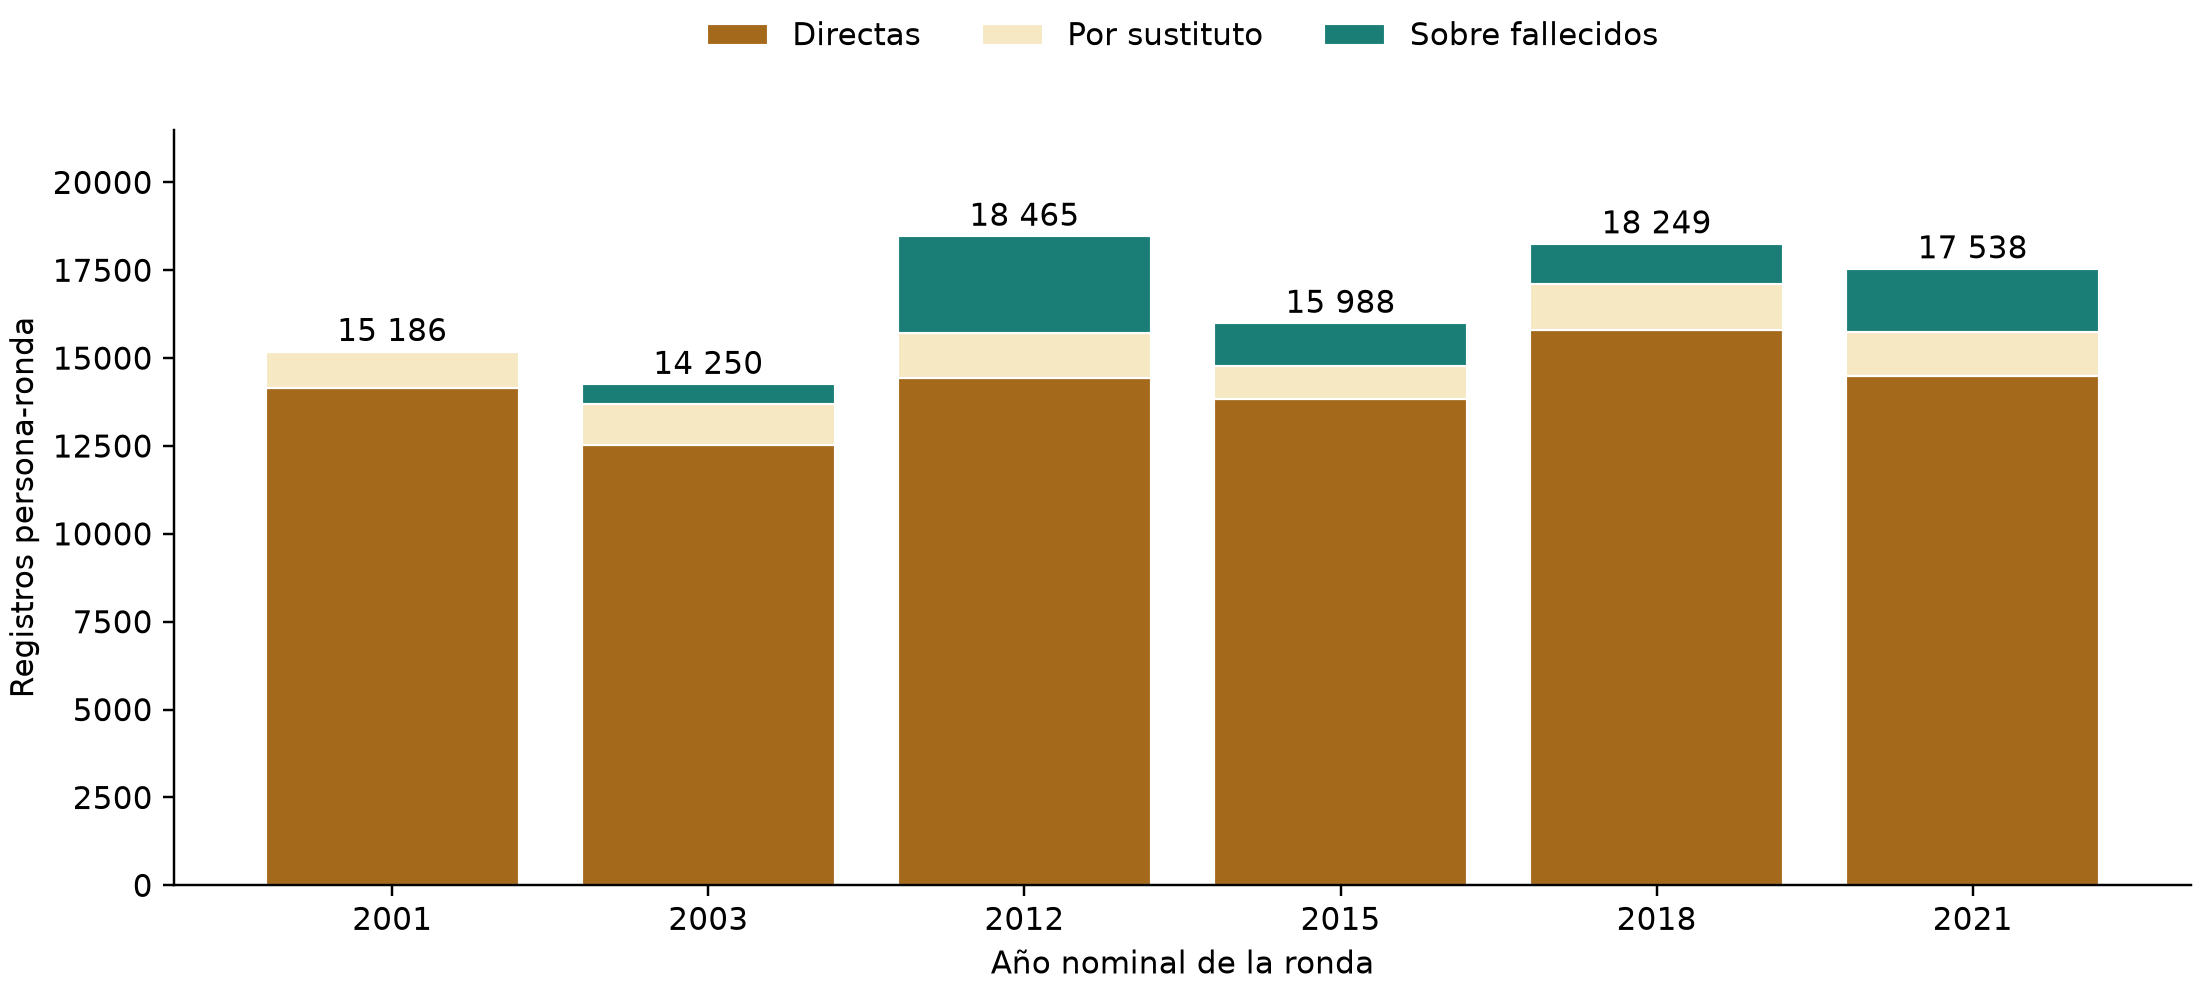
\includegraphics[width=\linewidth]{../resultados/figuras/figuras__borradores__cp1_modalidades.png}
 \caption[Registros por ronda y modalidad]{Registros por ronda y modalidad. Fuente: agregados de CP1, sin
 ponderación; todas las edades. Figura provisional para revisión editorial.}
 \label{fig:modalidades}
\end{figure}

\section{Incorporación, continuidad y ausencias temporales}

La primera aparición de una persona en el archivo se identifica mediante
$E_i=\min\{r:R_{ir}=1\}$. En una ronda, son incorporaciones observadas quienes
tienen $E_i=r$; son participantes previos quienes tienen $E_i<r$. Una
reaparición cumple simultáneamente presencia actual, presencia en alguna
ronda anterior y ausencia en la ronda inmediata precedente. Estas
definiciones dependen de la historia de registro, no de suponer equivalencia
con los códigos de muestra nueva del proveedor.

% Generado: no editar cifras manualmente.
\begin{table}[!htbp]
\centering
\caption{Incorporación y seguimiento por ronda}\label{tab:cp1-entradas}
\small\setlength{\tabcolsep}{4pt}
\renewcommand{\arraystretch}{1.15}
\begin{tabular}{lrrrr}
\toprule
\textbf{Año} & \textbf{N} & \shortstack[c]{\textbf{Primera}\\\textbf{presencia}} & \shortstack[c]{\textbf{Presencia}\\\textbf{previa}} & \textbf{Reaparición} \\
\midrule
2001 & 15\,186 & \shortstack[r]{15\,186\\(100,00\%)} & \shortstack[r]{0\\(0,00\%)} & \shortstack[r]{0\\(0,00\%)} \\
2003 & 14\,250 & \shortstack[r]{277\\(1,94\%)} & \shortstack[r]{13\,973\\(98,06\%)} & \shortstack[r]{0\\(0,00\%)} \\
2012 & 18\,465 & \shortstack[r]{5\,912\\(32,02\%)} & \shortstack[r]{12\,553\\(67,98\%)} & \shortstack[r]{357\\(1,93\%)} \\
2015 & 15\,988 & \shortstack[r]{650\\(4,07\%)} & \shortstack[r]{15\,338\\(95,93\%)} & \shortstack[r]{624\\(3,90\%)} \\
2018 & 18\,249 & \shortstack[r]{4\,823\\(26,43\%)} & \shortstack[r]{13\,426\\(73,57\%)} & \shortstack[r]{383\\(2,10\%)} \\
2021 & 17\,538 & \shortstack[r]{323\\(1,84\%)} & \shortstack[r]{17\,215\\(98,16\%)} & \shortstack[r]{1\,100\\(6,27\%)} \\
\bottomrule
\end{tabular}
\par\medskip
\parbox{\linewidth}{\footnotesize Fuente: elaboración propia con agregados de CP1, ENASEMsimple v2 (2001--2021). Frecuencias sin ponderación. Porcentajes sobre N de la ronda. Primera presencia + presencia previa = N. Reaparición es un subconjunto de presencia previa; primera presencia en el archivo no equivale automáticamente a modalidad de muestra nueva.}
\end{table}


La tabla~\ref{tab:cp1-entradas} permite reconciliar primeras apariciones y
participación previa con cada total. En 2012 hay \cpEntradasTres{} primeras
presencias y en 2018 \cpEntradasCinco{}, lo que contribuye al cambio de
composición respecto a las rondas anteriores. Las reapariciones suman
\cpReaparicionesTres{} en 2012, \cpReaparicionesCuatro{} en 2015,
\cpReaparicionesCinco{} en 2018 y \cpReaparicionesSeis{} en 2021. Son un
subconjunto de quienes ya habían participado, de modo que no deben sumarse
otra vez al total ni clasificarse como incorporaciones nuevas.

Para rondas consecutivas, la retención descriptiva se calcula como
\begin{equation}
 \widehat\rho_{r,r+1}=
 \frac{\sum_i R_{ir}R_{i,r+1}}{\sum_i R_{ir}}.
 \label{eq:retencion}
\end{equation}
El numerador incluye cualquier registro en destino. En consecuencia,
$\widehat\rho$ mide continuidad de presencia y no supervivencia. Las
entrevistas sobre fallecidos permanecen en el universo; un cambio de
modalidad no se confunde con ausencia.

% Generado: no editar cifras manualmente.
\begin{table}[!htbp]
\centering
\caption{Continuidad entre rondas nominales consecutivas}\label{tab:cp1-transiciones}
\small\setlength{\tabcolsep}{4pt}
\renewcommand{\arraystretch}{1.15}
\begin{tabular}{lrrrrr}
\toprule
\textbf{Transición} & \textbf{Años} & \textbf{N origen} & \textbf{Continúan} & \textbf{Retención (\%)} & \textbf{Ausentes} \\
\midrule
2001--2003 & 2 & 15\,186 & 13\,973 & 92,01 & 1\,213 \\
2003--2012 & 9 & 14\,250 & 12\,196 & 85,59 & 2\,054 \\
2012--2015 & 3 & 18\,465 & 14\,714 & 79,69 & 3\,751 \\
2015--2018 & 3 & 15\,988 & 13\,043 & 81,58 & 2\,945 \\
2018--2021 & 3 & 18\,249 & 16\,115 & 88,31 & 2\,134 \\
\bottomrule
\end{tabular}
\par\medskip
\parbox{\linewidth}{\footnotesize Fuente: elaboración propia con agregados de CP1, ENASEMsimple v2 (2001--2021). Frecuencias sin ponderación. Continúan + ausentes = N origen. La retención usa cualquier modalidad en destino, incluidas entrevistas sobre fallecidos. Los intervalos no son iguales y los porcentajes no son tasas anuales.}
\end{table}

% Generado: no editar cifras manualmente.
\begin{table}[!htbp]
\centering
\caption{Descomposición de las ausencias y retornos posteriores}\label{tab:cp1-ausencias}
\small\setlength{\tabcolsep}{4pt}
\renewcommand{\arraystretch}{1.15}
\begin{tabular}{lrrrr}
\toprule
\textbf{Transición} & \shortstack[c]{\textbf{Con}\\\textbf{fallecimiento}} & \shortstack[c]{\textbf{Sin}\\\textbf{fallecimiento}} & \shortstack[c]{\textbf{Retorno}\\\textbf{posterior}} & \shortstack[c]{\textbf{Sin retorno}\\\textbf{registrado}} \\
\midrule
2001--2003 & 0 & 1\,213 & 402 & 811 \\
2003--2012 & 546 & 1\,508 & 603 & 1\,451 \\
2012--2015 & 2\,741 & 1\,010 & 393 & 3\,358 \\
2015--2018 & 1\,209 & 1\,736 & 1\,066 & 1\,879 \\
2018--2021 & 1\,135 & 999 & 0 & 2\,134 \\
\bottomrule
\end{tabular}
\par\medskip
\parbox{\linewidth}{\footnotesize Fuente: elaboración propia con agregados de CP1, ENASEMsimple v2 (2001--2021). Frecuencias sin ponderación. Las dos primeras columnas de conteos dividen las ausencias según tipent=5 en la ronda inmediatamente anterior. Las dos últimas dividen esas mismas ausencias según retorno posterior observado; no sumar las cuatro. Sin retorno registrado no significa pérdida definitiva; 2021 es el cierre del archivo.}
\end{table}


La tabla~\ref{tab:cp1-transiciones} muestra variación en continuidad, con
intervalos nominales diferentes. La tabla~\ref{tab:cp1-ausencias} separa
ausencias tras una entrevista sobre fallecido en la ronda inmediatamente
anterior y ausencias sin ese antecedente. Esta segunda categoría no tiene
causa identificada por la comparación. También se examina retrospectivamente
qué ausencias son seguidas por una presencia posterior: ello demuestra
ausencia temporal de registro, pero no su causa ni supervivencia. La ausencia
sin retorno documentado hasta 2021 tampoco se denomina pérdida definitiva,
pues el archivo tiene un límite de observación.

Estas distinciones son esenciales para formular pares prospectivos. El
fallecimiento podría impedir observar un resultado económico de la misma
naturaleza; la sustitución podría cambiar la medición disponible; la ausencia
podría generar un resultado no observado. No se asignará la misma etiqueta a
estos procesos sin definir previamente el estimando. El tratamiento de muerte,
sustitución y ausencia permanece pendiente de revisión metodológica.

\section{Patrones de observación y atrición}

% Generado: no editar cifras manualmente.
\begin{table}[!htbp]
\centering
\caption{Número de rondas observadas por persona}\label{tab:cp1-participacion}
\small\setlength{\tabcolsep}{4pt}
\renewcommand{\arraystretch}{1.15}
\begin{tabular}{lrr}
\toprule
\shortstack[c]{\textbf{Rondas}\\\textbf{observadas}} & \textbf{Personas} & \textbf{Porcentaje} \\
\midrule
1 & 2\,025 & 7,45 \\
2 & 6\,635 & 24,42 \\
3 & 4\,445 & 16,36 \\
4 & 5\,589 & 20,57 \\
5 & 2\,172 & 7,99 \\
6 & 6\,305 & 23,20 \\
\bottomrule
\end{tabular}
\par\medskip
\parbox{\linewidth}{\footnotesize Fuente: elaboración propia con agregados de CP1, ENASEMsimple v2 (2001--2021). Frecuencias sin ponderación. Denominador: 27,171 personas únicas de 2001--2021. Presencia incluye cualquier modalidad; no equivale a entrevista directa.}
\end{table}


La distribución de $K_i$ en la tabla~\ref{tab:cp1-participacion} muestra que
\cpBalancePersonas{} personas aparecen en las seis rondas, equivalentes a
\cpBalancePorcentaje{} del universo de personas. La presencia en menos
rondas puede reflejar entrada tardía, fallecimiento, ausencia temporal o
cierre del seguimiento. El número de rondas no es, por sí mismo, una medida
de incumplimiento o abandono. La matriz individual de presencia se conserva
solo para cálculo interno; el notebook presenta intersecciones y patrones
agregados, sin identificadores.

\begin{figure}[tbp]
 \centering
 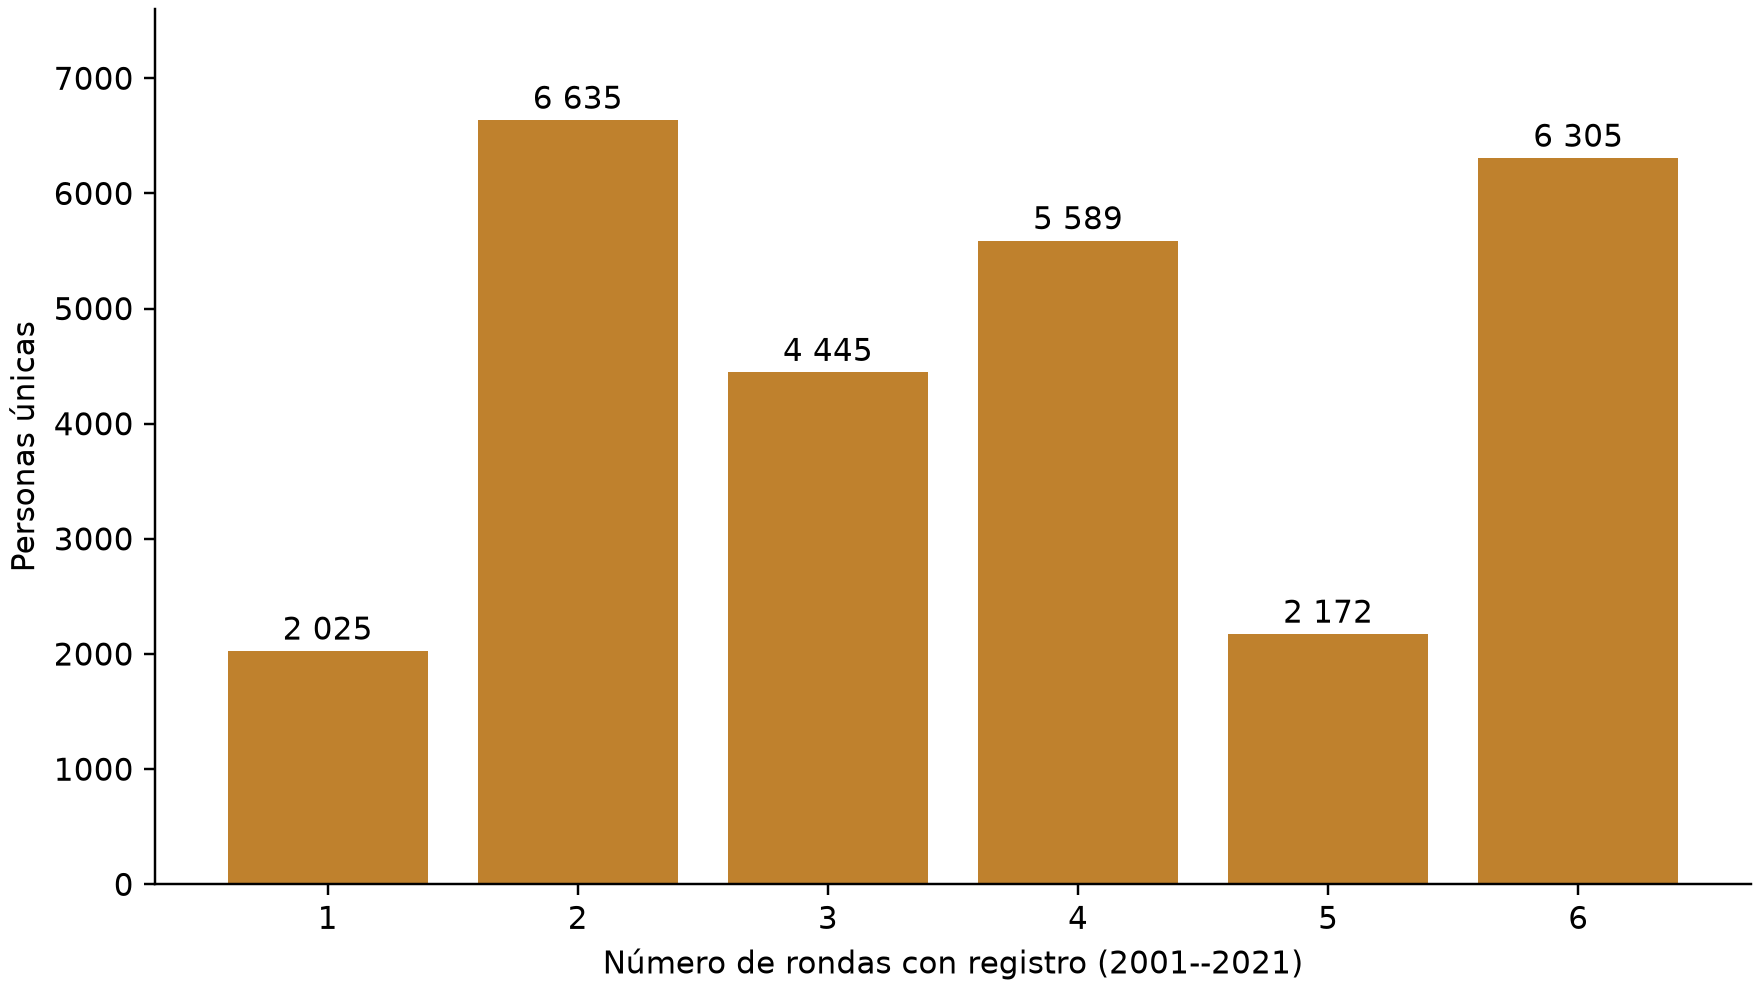
\includegraphics[width=0.90\linewidth]{../resultados/figuras/figuras__borradores__cp1_participacion.png}
 \caption[Personas según número de rondas con registro]{Personas según número de rondas con registro. Denominador:
 \cpTotalPersonas{} personas únicas; cualquier modalidad. Fuente: CP1, sin
 ponderación. Figura provisional para revisión editorial.}
 \label{fig:participacion}
\end{figure}

La continuidad completa selecciona una trayectoria futura y excluye entradas
tardías aun cuando tengan mediciones utilizables. Por esta razón no se
interpreta el panel completo como representativo por defecto. Las comparaciones
descriptivas de edad entre observados y ausentes en la ronda siguiente también
dependen de quién dispone de edad válida; los fallecidos permanecen en los
denominadores y a menudo no tienen esa variable. Estos contrastes sugieren
examinar selección, pero no estiman un efecto de la edad sobre abandono ni
cuantifican todavía sesgo en un modelo predictivo. El ajuste por atrición será
una evaluación posterior con supuestos explícitos.

\section{Valores faltantes, cobertura y ponderación}

La carga de Stata preserva los valores faltantes especiales antes de generar
una vista numérica para estadísticos. Se distinguen \variable{.f}
(reportado fallecido), \variable{.p} (información no incluida por sustituto),
\variable{.w} (no formulada en esa ronda), y las restantes causas de falta de
respuesta o invalidez del diccionario \citep{enasem2025simple}. Su reducción
prematura a un único faltante impediría distinguir indisponibilidad
estructural de falta de respuesta. No se convierten en cero ni se imputan
como parte de CP1.

% Generado: no editar cifras manualmente.
\begin{table}[!htbp]
\centering
\caption{Cobertura numérica de variables seleccionadas}\label{tab:cp1-cobertura}
\small\setlength{\tabcolsep}{4pt}
\renewcommand{\arraystretch}{1.15}
\begin{tabular}{p{0.20\linewidth}rrrrrr}
\toprule
\textbf{Variable} & \textbf{2001} & \textbf{2003} & \textbf{2012} & \textbf{2015} & \textbf{2018} & \textbf{2021} \\
\midrule
edad & \shortstack[r]{15\,186\\(100,00\%)} & \shortstack[r]{13\,693\\(96,09\%)} & \shortstack[r]{15\,701\\(85,03\%)} & \shortstack[r]{14\,775\\(92,41\%)} & \shortstack[r]{17\,094\\(93,67\%)} & \shortstack[r]{15\,729\\(89,69\%)} \\
sexo & \shortstack[r]{15\,186\\(100,00\%)} & \shortstack[r]{14\,250\\(100,00\%)} & \shortstack[r]{18\,465\\(100,00\%)} & \shortstack[r]{15\,988\\(100,00\%)} & \shortstack[r]{18\,249\\(100,00\%)} & \shortstack[r]{17\,538\\(100,00\%)} \\
educacion & \shortstack[r]{15\,167\\(99,87\%)} & \shortstack[r]{14\,151\\(99,31\%)} & \shortstack[r]{18\,371\\(99,49\%)} & \shortstack[r]{15\,808\\(98,87\%)} & \shortstack[r]{18\,089\\(99,12\%)} & \shortstack[r]{17\,214\\(98,15\%)} \\
est\_conyugal & \shortstack[r]{14\,730\\(97,00\%)} & \shortstack[r]{13\,703\\(96,16\%)} & \shortstack[r]{15\,723\\(85,15\%)} & \shortstack[r]{14\,779\\(92,44\%)} & \shortstack[r]{17\,114\\(93,78\%)} & \shortstack[r]{15\,739\\(89,74\%)} \\
urbano & \shortstack[r]{15\,186\\(100,00\%)} & \shortstack[r]{13\,704\\(96,17\%)} & \shortstack[r]{15\,723\\(85,15\%)} & \shortstack[r]{14\,779\\(92,44\%)} & \shortstack[r]{17\,114\\(93,78\%)} & \shortstack[r]{15\,739\\(89,74\%)} \\
a\_o\_ent & \shortstack[r]{15\,186\\(100,00\%)} & \shortstack[r]{14\,250\\(100,00\%)} & \shortstack[r]{15\,721\\(85,14\%)} & \shortstack[r]{14\,779\\(92,44\%)} & \shortstack[r]{17\,114\\(93,78\%)} & \shortstack[r]{15\,739\\(89,74\%)} \\
imp\_neto & \shortstack[r]{15\,127\\(99,61\%)} & \shortstack[r]{13\,671\\(95,94\%)} & \shortstack[r]{15\,723\\(85,15\%)} & \shortstack[r]{14\,745\\(92,23\%)} & \shortstack[r]{17\,094\\(93,67\%)} & \shortstack[r]{15\,716\\(89,61\%)} \\
orientacion & \shortstack[r]{0\\(0,00\%)} & \shortstack[r]{12\,495\\(87,68\%)} & \shortstack[r]{14\,448\\(78,25\%)} & \shortstack[r]{13\,850\\(86,63\%)} & \shortstack[r]{15\,786\\(86,50\%)} & \shortstack[r]{14\,484\\(82,59\%)} \\
serial7 & \shortstack[r]{0\\(0,00\%)} & \shortstack[r]{0\\(0,00\%)} & \shortstack[r]{0\\(0,00\%)} & \shortstack[r]{13\,850\\(86,63\%)} & \shortstack[r]{15\,786\\(86,50\%)} & \shortstack[r]{14\,484\\(82,59\%)} \\
\bottomrule
\end{tabular}
\par\medskip
\parbox{\linewidth}{\footnotesize Fuente: elaboración propia con agregados de CP1, ENASEMsimple v2 (2001--2021). Frecuencias sin ponderación. Cada celda: n válido y (\% sobre el total de la ronda). Se refiere a cobertura empírica, no a universo elegible ni respuesta entre vivos. El resto conserva sus motivos de faltante en los notebooks; cero valores válidos no equivale a ausencia del atributo.}
\end{table}


La tabla~\ref{tab:cp1-cobertura} presenta un subconjunto informativo de las
119 columnas auditadas. La cobertura varía por ronda y modalidad; tener una
columna no significa que su pregunta haya sido administrada a toda la muestra.
En particular, los ceros de cobertura de pruebas cognitivas en rondas sin
medición no indican ausencia de dificultad cognitiva. El inventario exhaustivo
de cada código y variable permanece en las seis fichas del notebook. Para
estadísticos continuos se utiliza el número de valores válidos, mientras que
las distribuciones categóricas conservan los faltantes dentro del total.

Los factores individuales \variable{factori_XX} y de hogar
\variable{factorh_XX} se auditan separadamente. Existen ceros y valores
positivos incluso en modalidades sobre fallecidos; la disponibilidad numérica
de un factor no acredita su pertinencia para un estimando dado. Todas las
tablas de este capítulo son frecuencias sin ponderación. No se suman factores
para llamarlos personas observadas, ni se trasladan factores transversales al
seguimiento como si fueran pesos longitudinales. El alcance de inferencia
poblacional exige una decisión adicional sobre universo, diseño y atrición.

\section{Auditoría de edad, sexo y fallecimiento}

% Generado: no editar cifras manualmente.
\begin{table}[!htbp]
\centering
\caption{Alertas de consistencia y denominadores}\label{tab:cp1-anomalias}
\small\setlength{\tabcolsep}{4pt}
\renewcommand{\arraystretch}{1.15}
\begin{tabular}{p{0.72\linewidth}r}
\toprule
\textbf{Control} & \textbf{n} \\
\midrule
Registros posteriores a primer fallecimiento & 3 \\
Personas con registros posteriores & 1 \\
Personas con códigos de sexo distintos & 1 \\
Pares adyacentes observados & 72\,505 \\
Pares con ambas edades válidas & 65\,031 \\
Pares con edad decreciente & 226 \\
Personas con edad decreciente & 225 \\
Pares que pasan de 60+ a menos de 60 & 48 \\
\bottomrule
\end{tabular}
\par\medskip
\parbox{\linewidth}{\footnotesize Fuente: elaboración propia con agregados de CP1, ENASEMsimple v2 (2001--2021). Frecuencias sin ponderación. Conteos agregados sin historias individuales. No se corrigen ni eliminan observaciones; una alerta no identifica cuál valor es correcto.}
\end{table}


La tabla~\ref{tab:cp1-anomalias} resume alertas sin corregir registros. Para
fallecimiento se identifica la primera ronda con \variable{tipent}=5 de cada
persona y se cuentan observaciones de rondas estrictamente posteriores.
Se detectan \cpMuerteRegistros{} registros posteriores de
\cpMuertePersonas{} persona: \cpMuerteDirectas{} directos y
\cpMuerteRepetidas{} nuevamente sobre fallecido.
Esta misma persona aporta la alerta de fallecimiento repetido. No son tres
personas ni duplicados de clave. La coincidencia de los dos indicadores
contemporáneos de fallecimiento no resuelve la contradicción longitudinal.
Son hipótesis posibles una clasificación de seguimiento incorrecta, una
revisión no propagada o un problema de enlace; falta contrastar el maestro,
las modalidades originales y la documentación de muerte. No se infiere una
fecha de muerte a partir de un año efectivo faltante.

Para sexo se cuenta el número de códigos válidos distintos dentro de una
persona. La alerta afecta a \cpSexoPersonas{} persona con \cpSexoRegistros{} registros
directos y códigos distintos; una moda no resuelve el empate. El proveedor
documenta que revisó sexo en la versión 2 mediante validación de discrepancias
de las variables originales \variable{sex_xx}
\citep[pp.~6--7]{enasem2025simple}. Se necesita verificar versión, variables
originales y enlace antes de decidir qué valor debe prevalecer. La alerta
no permite atribuir una causa individual.

Para edad se ordenan las observaciones por persona y ronda. Sea $r_i^{-}$
la ronda del registro observado inmediatamente anterior: se identifica un
descenso cuando
\begin{equation}
 D_{ir}=\mathbf{1}\{e_{ir}<e_{i,r_i^{-}}\},
 \quad \text{si ambas edades son numéricas válidas}.
 \label{eq:descenso-edad}
\end{equation}
Una ronda sin registro puede saltarse; una edad ausente en un registro
presente interrumpe la comparación y no se reemplaza por una edad válida
más antigua. De \cpParesObservados{} pares observados,
\cpEdadEvaluables{} son evaluables y \cpEdadNoEvaluables{} no.
Se reproducen \cpEdadPares{} descensos (\cpEdadPorcentaje{} de los pares
evaluables) en \cpEdadPersonas{} personas. Hay \cpEdadConsecutivos{} pares
entre rondas consecutivas y \cpEdadHuecos{} separados por una ronda ausente.
En \cpEdadCruce{} pares se pasa de edad registrada de 60 o más a menos de
60, con posible impacto en la elegibilidad por visita.

Todos los pares decrecientes presentan años efectivos crecientes y años de
nacimiento válidos sin cambios. Un contraste auxiliar comprueba si la edad
está en $[a_{ir}-b_{ir}-1,\ a_{ir}-b_{ir}]$, donde $b_{ir}$ es el año de
nacimiento declarado. En \cpEdadAnteriorIncompatible{} pares la edad anterior es incompatible y la
actual compatible, en \cpEdadActualIncompatible{} sucede lo contrario y en
\cpEdadAmbasIncompatibles{} ambas son incompatibles.
El intervalo es aproximado y depende de la veracidad de los años; no decide
qué edad es correcta ni certifica nacimiento. Un cumpleaños no explica por
sí solo un descenso cuando el año de entrevista avanza y el nacimiento
permanece estable. La magnitud, el modo de entrevista y los agregados
complementarios están documentados en el informe de revisión y el notebook.

La edad creada debe cotejarse con respuestas originales, fechas y reglas de
derivación. No se fuerza monotonicidad, no se reconstruye automáticamente
edad con nacimiento y no se eliminan casos. La ausencia de descenso tampoco
valida aumentos implausibles. Todas las alertas requieren un protocolo de
verificación antes de traducirse en reglas de inclusión o etiquetas.

\section{Comparación de alternativas de muestra}

% Generado: no editar cifras manualmente.
\begin{table}[!htbp]
\centering
\caption{Alternativas de muestra en todo el periodo}\label{tab:cp1-muestras}
\small\setlength{\tabcolsep}{4pt}
\renewcommand{\arraystretch}{1.15}
\begin{tabular}{p{0.24\linewidth}rrrrr}
\toprule
\textbf{Alternativa} & \textbf{Registros} & \textbf{Personas} & \textbf{\% personas} & \shortstack[c]{\textbf{Reg.}\\\textbf{excluidos}} & \shortstack[c]{\textbf{Pers.}\\\textbf{excluidas}} \\
\midrule
Universo completo & 99\,676 & 27\,171 & 100,00 & 0 & 0 \\
No balanceado & 99\,676 & 27\,171 & 100,00 & 0 & 0 \\
60+ por visita & 56\,004 & 18\,754 & 69,02 & 43\,672 & 8\,417 \\
Directas & 85\,248 & 26\,572 & 97,80 & 14\,428 & 599 \\
Directas 60+ & 50\,841 & 18\,158 & 66,83 & 48\,835 & 9\,013 \\
Seis presencias & 37\,830 & 6\,305 & 23,20 & 61\,846 & 20\,866 \\
Seis directas & 23\,358 & 3\,893 & 14,33 & 76\,318 & 23\,278 \\
Seis directas 60+ & 5\,784 & 964 & 3,55 & 93\,892 & 26\,207 \\
\bottomrule
\end{tabular}
\par\medskip
\parbox{\linewidth}{\footnotesize Fuente: elaboración propia con agregados de CP1, ENASEMsimple v2 (2001--2021). Frecuencias sin ponderación. Denominadores: 99,676 registros y 27,171 personas únicas. Personas conservadas: unión de claves con al menos una observación elegible. Cada filtro se compara independientemente con el universo; no hay una muestra predictiva aprobada.}
\end{table}


La tabla~\ref{tab:cp1-muestras} compara filtros independientes con el universo
original. El panel no balanceado permite de una a seis presencias y coincide
aquí con todo el universo; no significa excluir a quienes tienen seis rondas.
El filtro de 60+ por visita conserva \cpMayoresRegistros{} registros de
\cpMayoresPersonas{} personas, mientras que el filtro de directas conserva
\cpDirectasRegistros{} y \cpDirectasPersonas{}, respectivamente. La
intersección directa 60+ conserva \cpDirectasMayoresRegistros{} registros de
\cpDirectasMayoresPersonas{} personas. Estas personas únicas son la unión de
quienes mantienen al menos una observación elegible, no la suma de los
conteos anuales.

Exigir seis presencias conserva \cpBalanceRegistros{} registros de
\cpBalancePersonas{} personas; exigir seis directas reduce a
\cpBalanceDirectasRegistros{} y \cpBalanceDirectasPersonas{}; exigir además
60+ en cada visita reduce a \cpBalanceDirectasMayoresRegistros{} y
\cpBalanceDirectasMayoresPersonas{}. Los filtros cambian simultáneamente
continuidad, modalidad y composición por edad. No son definiciones
intercambiables y no se aprueba aquí ninguna muestra predictiva principal.
El apéndice~\ref{ap:tablas-cp1} muestra conservados y excluidos por ronda,
reconciliados con cada total original.

Otros criterios, como ser 60+ en la primera observación o permitir ingreso
desde la primera edad elegible, siguen comparados en el notebook. Su elección
dependerá de qué población y tiempo de entrada se pretenda representar.
Una alerta prospectiva no puede seleccionar observaciones por información
futura sin reconocer y justificar esa selección.

\section{Limitaciones y decisiones pendientes}

La unicidad de claves hace auditable el enlace, pero no garantiza veracidad
de todos los atributos. La cobertura heterogénea restringe qué predictores
pueden compararse entre rondas; las entrevistas por sustituto y sobre
fallecidos no proporcionan mediciones equivalentes a las directas. Las
primeras apariciones describen el archivo y no prueban todas las razones
institucionales de incorporación. La ausencia sin causa registrada y el
cierre en 2021 impiden clasificar pérdidas definitivas únicamente con los
patrones de presencia. Las frecuencias sin ponderación no se interpretan
como estimaciones nacionales.

Para el diseño económico, \variable{imp_neto} es patrimonio de la persona
y su cónyuge cuando corresponde, no un flujo de ingreso. Su uso exige
verificar precios, unidades, imputaciones y comparabilidad entre rondas antes
de establecer un umbral. Una posición relativa baja es una candidata
operativa que no se equipara sin discusión a pobreza ni a la medida de
vulnerabilidad de \citet{ligon2003}. Quedan pendientes el estimando, criterio
de edad/entrada, modalidad admisible, tratamiento de muerte y no observación,
alcance de ponderación y reglas de anomalías.

La futura comparación de modelos seguirá el protocolo del proyecto: misma
muestra de evaluación, mismos horizontes y particiones, transformaciones
aprendidas solo en entrenamiento e incertidumbre que respete dependencia
por persona. Se documenta aquí como requisito, no como validación ya ejecutada.
El cierre metodológico de CP1 sigue pendiente de revisión. La autora autorizó
iniciar el EDA independiente por bloques el 12 de octubre de 2026; esta autorización
no aprueba el estimando ni la integración definitiva. La escritura acompaña los resultados disponibles
sin convertir propuestas en decisiones definitivas.

% BEGIN CONSOLIDATED 03_pensiones_metodo
\section{Fuentes económicas y protocolo de clasificación pensionaria}
\label{sec:pensiones-metodo}

Los apartados siguientes conservan el protocolo documental anterior a la
integración. Su descripción de un enlace futuro debe leerse como antecedente
metodológico; la ejecución provisional y sus resultados se documentan en la
sección~\ref{sec:integracion-provisional}. El inventario nacional ampliado
se presenta en la sección~\ref{sec:catalogo-nacional}. Las condiciones de
validación no implican que se haya aprobado una homologación definitiva.


El complemento pensionario comienza con una auditoría de fuentes separadas,
antes de construir una base económica integrada. Se inspeccionaron completos
los 20 archivos Stata proporcionados: originales de K, archivos imputados,
secciones K individuales construidas, combinados de G/J/K/SA y ENASEMsimple.
También se revisaron las seis hojas del inventario Excel disponible. Las
fuentes contienen 5,368 columnas fuente-variable, incluidas las dos copias
individuales de 2018 y el archivo de 2024. El conteo describe cobertura del
inventario, no variables distintas ni observaciones independientes.

La lectura preservó las etiquetas y los valores faltantes especiales de Stata,
sin convertir categorías a textos. Para cada columna se registraron tipo,
etiqueta, conjunto de códigos etiquetados, número de filas y faltantes por
clase. Los códigos numéricos de negativa o desconocimiento permanecen sin
transformar: el número de valores no perdidos en Stata no equivale a un número
de respuestas sustantivas válidas. La determinación del universo elegible
requiere los saltos del instrumento. Esta etapa no calcula medias monetarias
que podrían incluir códigos numéricos especiales.

\begingroup\small\singlespacing
\setlength{\tabcolsep}{3pt}
\begin{longtable}{llrrp{4.4cm}}
\caption{Inventario de fuentes económicas revisadas}\label{tab:pensiones_fuentes}\\
\toprule \textbf{Fuente} & \textbf{Ronda} & \textbf{Registros} & \textbf{Variables} & \textbf{Clave única comprobada} \\
\midrule\endfirsthead
\toprule \textbf{Fuente} & \textbf{Ronda} & \textbf{Registros} & \textbf{Variables} & \textbf{Clave única comprobada} \\
\midrule\endhead\bottomrule\endfoot
F01 & 2012 & 10,427 & 164 & cunicah+subhog\_12 \\
F02 & 2015 & 9,921 & 212 & cunicah+subhog\_15 \\
F03 & 2021 & 10,716 & 180 & cunicah+subhog\_21 \\
F04 & 2018 & 17,094 & 125 & cunicah+np \\
F05 & 2018 & 17,094 & 125 & cunicah+np \\
F06 & 2024 & 14,076 & 507 & cunicah+subhog\_24 \\
F07 & 2012 & 10,427 & 648 & cunicah+subhog\_12 \\
F08 & 2015 & 9,953 & 756 & cunicah+subhog\_15 \\
F09 & 2018 & 11,401 & 543 & cunicah+subhog\_18 \\
F10 & 2021 & 10,716 & 524 & cunicah+subhog\_21 \\
F11 & 2003 & 8,895 & 348 & cunicah+acthog \\
F12 & 2001 & 9,811 & 328 & unhhid \\
F13 & 2001 & 15,186 & 62 & cunicah+codent01 \\
F14 & 2003 & 13,704 & 65 & cunicah+codent03 \\
F15 & 2012 & 15,723 & 66 & cunicah+np \\
F16 & 2015 & 14,779 & 156 & cunicah+np \\
F17 & 2021 & 15,739 & 129 & cunicah+np \\
F18 & 2003 & 8,895 & 165 & cunicah+acthog \\
F19 & 2001 & 9,811 & 146 & unhhid \\
F20 & 2001--2021 & 99,676 & 119 & cunicah+np+ronda \\
\end{longtable}
\noindent\footnotesize Fuentes F01--F20 se identifican por nombre completo en el inventario consolidado y su JSON. Ambas copias idénticas de 2018 se conservan. No sumar registros entre fuentes; existen universos solapados. El archivo 2024 queda separado.\par
\endgroup


El resumen de la tabla~\ref{tab:pensiones_fuentes} se acompaña de un diccionario
íntegro por archivo y una matriz variable--fuente, generados desde los metadatos.
La matriz contiene 1,917 candidatos léxicos tras retirar exclusivamente el sufijo
de ronda; esa operación facilita localizar columnas, pero no prueba equivalencia
conceptual. Todas las variables sustantivas quedan en el alcance del EDA futuro,
incluidos negocios, trabajo, activos, deuda, vivienda, donativos, gasto,
inseguridad alimentaria, apoyo familiar y los módulos de fallecimiento.
No se limita la revisión a ocho columnas finales.

\subsection{Unidad de observación y correspondencias comprobadas}

Los originales económicos y sus imputados tienen claves de entrevista de
hogar o subhogar; pueden contener flujos propios del informante, de su cónyuge
y conjuntos. Los archivos K individuales son productos construidos, no la
respuesta original de cada persona. La documentación del proveedor distingue
la construcción de ingresos individuales de la riqueza de hogar
\citep{enasemconstruidos,enasem2021imputacion}. Enlazar un hogar a dos personas
no autoriza adjudicar íntegramente un mismo monto a ambas.

Se comprobaron claves completas y únicas en todas las fuentes. Los individuales
de 2001 y 2003 usan, respectivamente, \variable{cunicah+codent01} y
\variable{cunicah+codent03}; los posteriores usan \variable{cunicah+np}.
Los originales de 2001 requieren un puente hacia \variable{unhhid}; los de
2003, un puente hacia \variable{cunicah+acthog} desde el individual construido.
El \variable{acthog} de ENASEMsimple no produce coincidencias directas con la
fuente económica de 2003. La coincidencia del nombre no garantiza la misma
codificación. Los ensayos de puente se limitaron a claves y validaron la
cardinalidad; no produjeron una base económica definitiva.

Todas las entrevistas directas de ENASEMsimple enlazan a los individuales
construidos en 2001, 2003, 2012, 2015 y 2021; en 2018 enlazan 15,766 de 15,786.
Los puentes a originales recuperan 14,099 de 14,154 directas en 2001 y 12,499
de 12,526 en 2003. En 2015 el original contiene 9,953 entrevistas económicas y
el imputado 9,921, y quedan 34 directas sin correspondencia en el imputado de
hogar. En 2021 hay 18 directas sin enlace al original/imputado de hogar,
aunque todas enlazan al individual. Estos resultados describen disponibilidad
y diferencias de universo, no ausencia de pensión o ingreso. La auditoría
completa conserva también los denominadores de todas las modalidades.

La huella SHA-256 acredita que las dos copias individuales de 2018 son
idénticas byte por byte. Ambas se inspeccionaron; no son dos muestras.
Las otras parejas de fuentes de la misma ronda se compararon por claves y
columnas comunes; el contraste de valores se restringió a claves únicas en
ambos lados. Las diferencias pueden reflejar imputación, derivación o versión,
y todavía no se atribuyen a una causa. El archivo imputado de hogar de 2018 y
los productos separados de ingreso total/patrimonio de 2018 y 2021 no se
identificaron entre los suministrados. Su existencia documental no acredita
su disponibilidad local.

\subsection{Definición de los ocho conceptos y estados de información}

Se mantienen las variables \variable{pension_contributiva},
\variable{pension_no_contributiva}, \variable{otro_apoyo_publico},
\variable{ayuda_familiar}, \variable{ingreso_pension_contributiva},
\variable{ingreso_pension_no_contributiva},
\variable{ingreso_transferencias_publicas} e \variable{ingreso_total}.
En esta entrega constituyen especificaciones de construcción: no se presentan
como variables armonizadas ya calculadas. La unidad objetivo es persona-ronda,
con titular, periodo, unidad monetaria y procedencia explícitos.

Los indicadores distinguirán recepción identificada, negativa explícita,
recepción de tipo desconocido, información faltante, pregunta no formulada
y no aplicabilidad. Solo una negativa con cobertura suficiente del concepto
permite codificar cero. Por ejemplo, desconocer el tipo de una pensión no
permite asignar simultáneamente cero a contributiva y no contributiva.
La recepción de una transferencia de una persona tampoco acredita parentesco.
Una prestación en especie se registra separadamente del flujo monetario.

\begin{table}[htbp]
\centering\small\singlespacing
\caption{Identificabilidad propuesta de los ocho conceptos económicos}\label{tab:pensiones_disponibilidad}
\begin{tabular}{p{5.1cm}cccccc}
\toprule \textbf{Concepto} & \textbf{2001} & \textbf{2003} & \textbf{2012} & \textbf{2015} & \textbf{2018} & \textbf{2021} \\
\midrule
pension contributiva & C & C & C & C & C & C \\
pension no contributiva & T & T & P & P & T & E \\
otro apoyo publico & P & P & P & P & C & C \\
ayuda familiar & T & T & C & C & C & C \\
ingreso pension contributiva & C & C & C & C & C & C \\
ingreso pension no contributiva & T & T & P & P & T & C \\
ingreso transferencias publicas & C & C & C & C & C & C \\
ingreso total & R & R & R & D & R & R \\
\bottomrule\end{tabular}
\par\medskip\begin{minipage}{\textwidth}\footnotesize
C: candidata condicionada; P: tipo parcial; T: agregado sin identificación suficiente; E: opción explícita de programa; D: total disponible del proveedor; R: reconstrucción o archivo adicional. No son resultados de recepción ni variables ya armonizadas.
\end{minipage}\end{table}


La tabla~\ref{tab:pensiones_disponibilidad} distingue la presencia física de
columnas de su identificabilidad. En 2001 se usan familias K55/K56/K58;
desde 2003 cambian a K58/K59/K61. En 2012 y 2015, las opciones de programas
federales o estatales permiten una clasificación parcial, sin nombre ni ámbito
inequívoco. En 2018, las fuentes de donativos públicos distinguen PROAGRO,
PROSPERA, INAPAM y otra institución, sin una opción explícita de pensión de
vejez. La opción de programas públicos en una pregunta de pensión futura no
prueba recepción actual \citep{inegi2018k}. En 2021 el cuestionario \citep{inegi2021k} incorpora una opción
explícita de Bienestar de personas adultas mayores en los apoyos propios y del
cónyuge. Esa mejora no elimina faltantes, ambigüedad de titular ni cambios del
periodo de referencia.

Los montos pensionarios agregados \variable{pens_t} o
\variable{inc_pension} no se tipifican automáticamente como contributivos.
Los totales \variable{tran_t} o \variable{inc_trans} tampoco equivalen sin
cotejo a transferencias exclusivamente públicas. Un mismo importe reportado,
derivado y luego imputado representa versiones de un componente; no se suman
como tres ingresos. Conservar las banderas de imputación permite evaluar la
sensibilidad en las mismas personas y periodos.

Para impedir doble conteo, el ingreso público incluye la prestación no
contributiva de vejez como un subconjunto. Una contabilidad propuesta es
\begin{equation}
 Y^{\mathrm{rec}}_{ir}=W_{ir}+B_{ir}+R_{ir}+C_{ir}
 +P^{\mathrm{con}}_{ir}+P^{\mathrm{sin\ tipo}}_{ir}
 +T^{\mathrm{pub}}_{ir}+T^{\mathrm{priv}}_{ir}+O_{ir},
 \label{eq:ingreso-componentes}
\end{equation}
donde trabajo, negocios, rentas, capital, pensiones y transferencias son
componentes mutuamente delimitados bajo una misma unidad y referencia.
$P^{\mathrm{no\ con}}$ no se vuelve a sumar porque está contenido en
$T^{\mathrm{pub}}$. La ecuación es una propuesta contable, no una definición
empírica aprobada: si falta un componente necesario, una suma parcial no se
presenta como ingreso total completo. \variable{income_15} existe en el
individual de 2015; los totales separados de 2018 y 2021 no están suministrados.
Los precios, periodicidades y fórmulas de los demás componentes deben cotejarse
antes de comparar cuantías entre rondas.

\subsection{Cronología, imputación y límites de integración}

La documentación de 2021 describe montos propios y de cónyuge, ingresos
individuales y riqueza de hogar, así como pasos adicionales que utilizan
información de 2018 para resolver ciertas atribuciones de 2021
\citep[pp.~6--8]{enasem2021imputacion}. Este antecedente obliga a conservar
procedencia y cronología del producto. No se supone que una imputación sea
una observación directa, ni que su disponibilidad retrospectiva garantice
que se hubiera conocido en el momento de una futura predicción. La ficha de
cada variable deberá registrar estas dependencias antes de usarla como señal
prospectiva.

La integración propuesta en el inventario conserva las 99,676 filas de ENASEMsimple mediante
uniones izquierdas validadas, sin sobrescribir edad, sexo, modalidad ni
cronología de CP1. Se exigirán relaciones uno-a-uno para fuentes individuales
y muchos-a-uno para hogar, indicadores de enlace y reconciliación de personas
y registros. Aún deben aprobarse titularidad, filtros, unidades, tratamiento
de fuentes no identificadas y equivalencias por pregunta. No se ha seleccionado
una muestra predictiva ni cambiado la definición económica pendiente.
La implementación provisional autorizada después de esa revisión se documenta
en la sección~\ref{sec:integracion-provisional}; no requiere cerrar primero
todos los bloques del EDA independiente.

El archivo de 2024 tiene 14,076 filas, 507 variables y clave única
\variable{cunicah+subhog_24}. Su fecha de versión en 2026 no es el año de ronda.
Se inventaría por separado: no existe una séptima ronda en el ENASEMsimple
proporcionado. Además, sus códigos de K79 distinguen vejez, discapacidad y ONG,
con numeración diferente de 2018 y 2021. Incorporarlo requeriría fuentes
individuales y puentes adicionales, revisión del instrumento y autorización
de la ampliación temporal. La referencia principal permanece en 2001--2021.
% END CONSOLIDATED 03_pensiones_metodo
% BEGIN CONSOLIDATED 03_eda_independiente_metodo
\section{Protocolo del análisis exploratorio independiente}
\label{sec:eda-independiente-metodo}

El análisis exploratorio se organiza en bloques de fuentes y rondas, conservando
la procedencia de cada medición. La autorización para iniciar esta etapa
descriptiva no establece una muestra predictiva, una definición de vulnerabilidad
ni una integración económica definitiva. La población registrada completa
continúa siendo la referencia; no se restringe inicialmente por edad, modalidad
de entrevista o continuidad de observación. Los resultados de integridad de CP1
conservan su alcance y sus decisiones pendientes.

La primera operación consiste en verificar que los archivos no hayan cambiado
respecto al inventario mediante sus sumas SHA-256, su estructura y sus conteos.
El control de cobertura incluye una fila por cada columna de cada fuente,
incluidas las copias idénticas y el archivo de 2024, que permanece fuera del
periodo principal. La prevalidación de códigos almacenados y faltantes se
distingue explícitamente del análisis sustantivo concluido. Los códigos de
negativa o desconocimiento se revisan por variable y cuestionario: no existe
una regla general que permita eliminar 8, 9, 88 o 99 en todas las mediciones.

En ENASEMsimple se elaboró un contrato por variable que identifica la página
del libro de códigos, la escala, la unidad, los códigos válidos y las
restricciones de interpretación \citep{enasem2025simple}. Los valores perdidos
especiales se contabilizan antes de la transformación numérica. La ausencia
de una pregunta, el salto por una respuesta previa, la entrevista por sustituto
y el fallecimiento se conservan como motivos distintos. Un valor fuera del
dominio documentado se registra separadamente; no se corrige ni se sustituye
automáticamente. Los valores extremos y los patrimonios negativos se mantienen.

Para una variable $v$ y ronda $t$, sea $N_t$ el número de registros y
$N^{\mathrm{val}}_{vt}$ el número con un valor disponible dentro del dominio
documentado. Para una categoría $c$, se presentan dos proporciones:
\begin{equation}
 p^{\mathrm{total}}_{vct}=\frac{n_{vct}}{N_t},
 \qquad
 p^{\mathrm{val}}_{vct}=\frac{n_{vct}}{N^{\mathrm{val}}_{vt}}.
 \label{eq:eda-denominadores}
\end{equation}
Ambas responden a preguntas distintas. La primera expresa la presencia de una
respuesta entre los registros de la ronda y la segunda describe la composición
de las respuestas válidas. Ninguna sustituye una proporción sobre el universo
elegible de la pregunta cuando este no se ha reconstruido. En particular, los
saltos laborales de \variable{autoem} y \variable{horas_trabajadas} requieren
cotejo adicional del instrumento; sus distribuciones se limitan a los valores
disponibles y no se presentan como prevalencias de toda la población.

La revisión posterior reconstruye el universo del indicador construido cuando
el libro documenta su disponibilidad por ronda y modalidad. Esta operación
conserva negativas, desconocimiento e interrupciones dentro del denominador
elegible; no utiliza el número de respuestas válidas como sustituto de dicho
universo. Si $N^{\mathrm{el}}_{vt}$ es el universo reconstruido y
$N^{\mathrm{val,el}}_{vt}$ las respuestas válidas en él, la cobertura es
$N^{\mathrm{val,el}}_{vt}/N^{\mathrm{el}}_{vt}$, definida solo si
$N^{\mathrm{el}}_{vt}>0$. Se auditan también valores válidos fuera del universo
propuesto. No disponibilidad instrumental implica universo cero y porcentaje
no definido; un filtro desconocido implica universo no determinado. Esta
distinción no reconstruye automáticamente todos los saltos de las preguntas
originales que alimentan el indicador.

Las medidas numéricas se describen mediante cuantiles, media, desviación
estándar, extremos y frecuencias de cero y valores negativos. Las categorías
nominales y ordinales se describen con frecuencias, sin interpretar la media
de sus códigos. Los histogramas emplean intervalos comunes entre rondas y
conservan las colas; el último intervalo incluye su extremo superior. Cada
lámina contiene seis paneles con la paleta BrBG y los denominadores explícitos.
Además se conserva una comparación conjunta por variable: porcentajes de todas
las categorías o P05, P25, mediana, P75 y P95 numéricos en una escala común,
junto con su tabla exacta. Los intervalos representan dispersión descriptiva,
no incertidumbre inferencial. Las ausencias no se grafican como tasas cero.
El desglose de modalidad distingue entrevistas directas de seguimiento y nuevas,
por sustituto de seguimiento y nuevas, y sobre fallecidos. Los porcentajes
son descriptivos sin ponderar y no constituyen estimaciones nacionales.

Las diferencias entre distribuciones de rondas describen composición, no
trayectorias individuales ni efectos causales. La escolaridad de primera
entrevista, las puntuaciones construidas y las banderas de imputación se
interpretan conforme a su procedencia. Antes de utilizar imputaciones del
proveedor como predictores será necesario verificar si su construcción empleó
información posterior al momento de la alerta. Esta etapa no demuestra ausencia
de fuga temporal ni estima desempeño predictivo. Tampoco compara crecimiento
patrimonial real mientras permanezcan pendientes las unidades, precios y
equivalencias entre fuentes económicas.

En el bloque independiente de K 2021, los montos derivados, imputados y las
banderas se cotejan dentro de cada archivo, sin unión definitiva entre fuentes.
Una recuperación corresponde a un derivado faltante con imputado disponible;
un cambio compara dos montos disponibles con tolerancia absoluta de 0.01 pesos
y relativa de $10^{-7}$. No se identifica de antemano la bandera con estas
operaciones: se verifica su concordancia empírica. Los ceros de productos
construidos pueden representar componentes no recibidos; su universo de
producto no es el universo de la pregunta monetaria entre receptores.
Los componentes del cónyuge requieren pareja: si el archivo carece del filtro,
el universo permanece no determinado. Cuando existe \variable{k52a_21},
el código 2 confirma pareja y el 1 excluye esa rama; una condición perdida
permanece desconocida. No se recupera el filtro de otra fuente mediante una
unión ni se deduce a partir de la disponibilidad del monto.

El cuestionario distingue la ventana retrospectiva de recepción de la
periodicidad solicitada para el monto. Negocios, rentas, pensiones ordinarias,
transferencias institucionales y consumo incluyen preguntas mensuales;
COVID y ventas/herencias solicitan montos totales. Los salarios permiten
periodo mensual o anual y su conversión no se da por validada sin verificar el
periodo del producto suministrado. Esta cautela responde a que el resumen
metodológico y el código del proveedor describen etapas distintas de
construcción \citep[pp.~4, 13--14 y apéndice]{enasem2021imputacion}.
En ningún caso se anualiza o deflacta automáticamente. La orientación de
ingresos propios o del cónyuge se audita solo mediante conteos internos de
punteros, sin publicar identificadores.
% END CONSOLIDATED 03_eda_independiente_metodo
% BEGIN CONSOLIDATED 03_integracion_provisional
\section{Integración longitudinal provisional de fuentes económicas}
\label{sec:integracion-provisional}

Tras revisar el inventario y los primeros análisis independientes, se autorizó
construir una base provisional sin esperar a terminar el EDA de todos los
archivos. Esta etapa resuelve la vinculación física y conserva la información
para nuevas verificaciones; no convierte la cobertura del enlace en validación
de titularidad, comparabilidad o elegibilidad de cada pregunta. La pregunta de
investigación y las decisiones predictivas pendientes permanecen vigentes.

\subsection{Identificación, cardinalidad y preservación del universo}

ENASEMsimple constituye el maestro de \intRegistros{} observaciones,
\intPersonas{} personas y seis rondas. Se conservan sus 119 variables, todas
las edades y modalidades, incluidos registros sobre fallecidos. La clave
personal es la concatenación estable de \variable{cunicah} y \variable{np}
con el separador ``:''; la observación queda identificada por
\variable{id+ronda}. Los componentes de texto conservan su formato y ceros
iniciales; los numéricos enteros se representan sin redondeo, relleno ni
notación científica. Se preservan también valores y formatos Stata del
maestro, sin reconstruir supuestos ceros iniciales de campos numéricos.
\variable{ano} representa la ronda nominal, mientras \variable{a_o_ent}
conserva el año efectivo de entrevista.

Para cada fuente económica $E_s$ se aplica una unión izquierda al maestro
$M$, validando la unicidad de la clave derecha antes del enlace:
\begin{equation}
M^{(s)}=M^{(s-1)}\;\mathop{\Join}\limits_{\mathrm{izquierda},\,k_s}\;E_s,
\qquad |M^{(s)}|=|M|.
\label{eq:integracion-izquierda}
\end{equation}
Las fuentes individuales requieren cardinalidad uno a uno dentro de ronda;
las fuentes de hogar admiten muchas personas hacia un único registro
económico. Claves incompletas no se emparejan entre sí y duplicados derechos
detienen el procedimiento. No se elige arbitrariamente una primera fila para
resolver conflictos ni se enlaza por \variable{cunicah} aisladamente.

En 2001, el individual construido enlaza mediante
\variable{cunicah+codent01} y aporta \variable{unhhid} para el hogar. En 2003,
\variable{cunicah+codent03} permite trasladar el \variable{acthog} económico;
el homónimo del maestro no produce una correspondencia directa válida. En
2012, 2015, 2018 y 2021 se emplean \variable{cunicah} y el subhogar específico
de cada ronda. Los puentes preservan el \variable{np} original del maestro.
Estos pasos se verifican individualmente en el notebook de integración.

\subsection{Procedencia, faltantes y titularidad}

Se incorporan \intFuentes{} fuentes económicas distintas, manteniendo
\intColumnasFuente{} columnas fuente, incluida la maestra. Cada campo
económico lleva el prefijo de su fuente y metadatos de producto original,
imputado o construido. La copia binaria idéntica del individual 2018 se
representa una vez con el alias documentado; 2024 sigue fuera del periodo.
Los indicadores de imputación y códigos originales desconocidos o no
aplicables se conservan, sin sumarlos como componentes adicionales.

Parquet almacena valores y etiquetas de faltantes Stata por separado. Un
auxiliar identifica el tag original cuando existe; el estado de enlace
distingue ausencia de fuente en la ronda, clave incompleta, falta de puente y
no correspondencia. Así, un null por unión no pierde su diferencia frente a
\variable{.f}, \variable{.p}, \variable{.w}, negativa o desconocimiento
numérico. Las cadenas vacías también se mantienen. Se comprueba la igualdad
de todas las columnas, filas y tags al releer el archivo, no solo su dimensión.

Un hogar puede aportar contexto económico a varias personas sin que sus
ingresos pertenezcan a todas ellas. La atribución personal se inicia en 2021,
cuyo instrumento y producto construido fueron cotejados
\citep{inegi2021k,enasem2021imputacion}. Se exige orientación
\variable{key_21}, coincidencia del NP del titular en hogar e individual y
rama de pareja válida. El puntero K45d por sí solo no enumera el bloque K58;
para pensiones se exige también la orientación del proveedor. Los registros
sobre fallecidos se conservan, pero no acreditan recepción personal actual.
Una discrepancia impide derivar el indicador y conserva los originales para
revisión.

Las preguntas afirmativas de pensión permiten conservar múltiples slots,
instituciones, año de inicio y montos observados mensuales; se mantienen los
casos de institución o monto desconocido. IMSS e ISSSTE identificados aportan
evidencia de sistema contributivo, incluyendo derechos derivados; no prueban
cotización personal ni régimen específico. Instituciones agrupadas,
privadas, extranjeras o personas permanecen sin tipo validado. La opción 5
de K79/K82 identifica el apoyo de vejez; otros programas públicos se
distinguen e INAPAM no se interpreta automáticamente como pensión monetaria.
El instrumento combina dinero y especie, limitación que se conserva.

El número derivado es un mínimo de declaraciones/slots con evidencia; una
suma observada es parcial y no ingreso total. No se añaden versiones
imputadas a los montos reportados ni se completa un faltante con cero.
Las demás rondas mantienen todas las columnas disponibles y una homologación
pendiente de titular, filtros, periodicidad y selección múltiple. Estas
variables auxiliares no cierran las ocho especificaciones previamente
acordadas ni resuelven el deflactor, ponderación o diseño prospectivo.
% END CONSOLIDATED 03_integracion_provisional
% BEGIN CONSOLIDATED 03_titularidad_pensiones
\section{Auditoría específica de titularidad pensionaria}
\label{sec:titularidad-metodo}

La vinculación de una entrevista económica de hogar con registros individuales
no determina por sí misma quién recibe una prestación. Esta auditoría distingue
la pensión del beneficiario de la fila, la recepción de su pareja residente y
la presencia de ingresos pensionarios declarados en la entrevista económica.
La unidad individual conserva la clave \texttt{id+ronda}, mientras que el
agregado económico utiliza la clave del hogar o subhogar de cada levantamiento.
El producto integrado anterior permanece intacto; se genera un conjunto de
auxiliares privados separado y versionado, sin eliminar variables fuente.

En las rondas tempranas, el proveedor describe una orientación de los ingresos
propios y de la pareja basada en controles de entrevista y códigos del informante.
En 2001 intervienen J1 y los controles de orden de entrevista; en 2003 se utiliza
K96a y el código personal histórico; en 2012 y 2015 se coteja K96a con NP
\citep{enasem2001imputacion,enasem2003imputacion,enasem2012imputacion,enasem2015imputacion}.
Los campos \texttt{key} de los productos individuales se verifican contra sus
componentes pensionarios construidos: una orientación relativa de la fila no
debe confundirse con los códigos absolutos de persona denominados CLAVE en
los documentos históricos. La concordancia numérica acredita el funcionamiento
de esa orientación, pero no sustituye los controles originales ausentes.
En particular, 2001 conserva una clasificación candidata del proveedor, con
comprobación independiente pendiente. Para informantes externos de 2003--2015
no se reproduce la asignación basada en orden de entrevista sin sus controles.

En 2018 y 2021, los punteros \texttt{k45d} y \texttt{k52a\_1} identifican por NP
a los titulares de las dos ramas económicas \citep{enasem2018imputacion,enasem2021imputacion}.
Se exige concordancia del puntero seleccionado entre el producto individual
y el original de hogar; en 2021 se coteja además \texttt{key\_21}. Si el NP del
sujeto corresponde a la rama de cónyuge, esa rama constituye su pensión propia,
aunque su pareja haya sido informante. Una rama no puede identificar a dos
personas distintas. La recepción de la pareja requiere cotejar también el otro
puntero y la rama de pareja; la concordancia del titular propio no resuelve
automáticamente el otro beneficiario. Los punteros discordantes, la orientación ausente y los
registros sobre fallecidos no acreditan recepción personal actual.

Los libros de códigos originales requieren un tratamiento monetario por ronda:
en 2001/2003 los montos pensionarios codifican negativa y desconocimiento como
888888 y 999999, mientras que desde 2012 utilizan 8888888 y 9999999
\citep{enasem2001codigosk,enasem2003codigosk}. Estos valores permanecen en la
fuente y se excluyen únicamente del monto analítico correspondiente.

El indicador de recepción K toma valor positivo ante una afirmativa en
jubilación, viudez, invalidez o accidente de trabajo, u otras pensiones; toma
valor negativo solo ante cuatro negativas explícitas. Las respuestas de
negativa a contestar, desconocimiento y los faltantes preservan su estado.
El filtro de ausencia de pareja residente se aplica solo cuando está
documentado en el archivo, sin deducirlo de respuestas ausentes. La recepción
del programa de vejez de 2021 se mantiene separada: K79/K82 admite dinero o
especie y una negativa del bloque K58/K64 no demuestra ausencia de toda
protección previsional \citep{inegi2021k}.

El doble conteo se controla mediante un registro lógico de prestaciones.
Sea $\mathcal{E}_{ht}$ el conjunto de slots originales únicos de un hogar
$h$ en la ronda $t$, distinguidos por rama beneficiaria y contingencia.
La suma observada parcial se define como
\begin{equation}
 M^{\mathrm{obs}}_{ht}=\sum_{e\in\mathcal{E}_{ht}:\,m_e\ \mathrm{observado}}m_e.
 \label{eq:titularidad-agregado}
\end{equation}
Este objeto descriptivo no es ingreso pensionario completo: excluye montos
desconocidos y no incorpora una segunda versión imputada del mismo slot.
Cuando no existe ningún monto observado, el agregado analítico es desconocido,
en lugar de cero. En el registro individual solo corresponden los eventos de
su beneficiario; la réplica de una pregunta de hogar en dos filas de personas
no genera dos prestaciones. En 2012/2015 las instituciones se seleccionan por
contingencia y no necesariamente identifican de forma unívoca cada slot.
Dos pensiones de igual institución e importe no se eliminan si corresponden a
beneficiarios o slots distintos.

La viudez se asigna a quien recibe efectivamente la prestación, no a la persona
fallecida que generó el derecho. Las preguntas sobre heredar en el futuro una
pensión no acreditan cobro. Los montos antes y después del fallecimiento
K101/K103 y las transferencias mixtas por divorcio, separación o supervivencia
se conservan como fuentes separadas y pendientes de reconciliación; no se
añaden automáticamente al bloque pensionario principal. Esta auditoría no
cierra las ocho especificaciones de armonización ni aprueba ponderación,
deflactor o muestra predictiva.
% END CONSOLIDATED 03_titularidad_pensiones
% BEGIN CONSOLIDATED 03_proteccion_economica
\section{Armonización descriptiva de pensiones y apoyos gubernamentales}
\label{sec:proteccion-metodo}

La protección económica se estudia mediante fuentes de recepción que complementan
el patrimonio y permiten describir su distribución entre perfiles demográficos.
Se reutilizan la base integrada provisional y la auditoría de titularidad de la
sección~\ref{sec:titularidad-metodo}; no se repiten las uniones ni se modifica el
maestro. La muestra descriptiva corresponde a edad de 60 años o más en cada visita,
sin exigir continuidad ni entrevista directa. Esta selección no aprueba la muestra
predictiva. Los registros sobre fallecidos no acreditan cobro contemporáneo y
permanecen en el universo longitudinal para estudiar seguimiento. La edad faltante
no permite establecer elegibilidad por edad y se contabiliza por separado.

Se definen dos indicadores documentales distintos. $P_{it}^{K}$ indica recepción
propia en las cuatro contingencias de K: jubilación, viudez, incapacidad y otra.
$A_{it}$ identifica donativos públicos adicionales en dinero o especie durante
el año previo a la entrevista. El bloque K no corresponde exclusivamente a
prestaciones contributivas y el bloque A no corresponde exclusivamente a
pensiones no contributivas. La pregunta sobre apoyos excluye el ingreso ya
mencionado; esta regla del instrumento no acredita que toda respuesta esté libre
de duplicación. No se construye un ingreso total sumando K y A.

En 2001 se utiliza K76a para el informante económico y K79a para su cónyuge;
en 2003 y desde 2012 se emplean K79a y K82c. Las ramas se orientan al beneficiario
auditado, que puede ocupar el apartado del cónyuge si respondió su pareja.
La orientación propia y el puntero de la otra persona se evalúan separadamente.
La respuesta 1 acredita recepción y 2 acredita negativa; NR, NS, faltantes y
enlaces no comprobados conservan estado desconocido. Ni un monto positivo ni
una imputación sustituyen la pregunta de recepción. Las reglas tempranas y sus
límites están documentados en \citet{enasem2001codigosk,enasem2003codigosk,
enasem2012imputacion,enasem2015imputacion}.

Hasta 2015 los donativos no identifican el programa individual: los ejemplos de
la pregunta no constituyen respuestas sobre programa. En 2018 se registran hasta
dos instituciones y en 2021 se agrega explícitamente el programa de vejez junto
con modificaciones de nombres \citep{inegi2018k,inegi2021k}.
Se conserva cada versión temporal. La opción 5 en 2021 identifica el programa de
vejez en este bloque, mientras INAPAM y una institución no especificada no se
convierten en una pensión monetaria. IMSS/ISSSTE acreditan la familia de seguridad
social, incluidas prestaciones derivadas; los demás organismos y regímenes
requieren evidencia adicional. Las categorías federales/estatales agrupadas de K
no permiten asignar nombre, ámbito ni monto individual por programa.

Los cruces distinguen recepción, coexistencia, apoyo con negativa K, apoyo con
pensión desconocida y negativas suficientes de los dos bloques. La última categoría
se denomina ``negativas K y A'', sin afirmar ausencia de toda prestación o ayuda
privada. Para un perfil $g$, se calculan por separado la proporción mínima observada
sobre el universo elegible y la tasa entre respuestas conocidas:
\begin{equation}
 \widehat r_{g,t}^{\mathrm{conocida}}=
 \frac{n_{g,t}^{\mathrm{si}}}{n_{g,t}^{\mathrm{si}}+n_{g,t}^{\mathrm{no}}},
 \qquad
 \widehat r_{g,t}^{\mathrm{elegible}}=
 \frac{n_{g,t}^{\mathrm{si}}}{N_{g,t}^{\mathrm{elegible}}}.
 \label{eq:proteccion-tasas}
\end{equation}
N elegible incluye personas vivas de 60+ en la visita; N conocido depende de
la recepción y de su cobertura documental. La composición de receptores emplea
otro denominador, $n_{g,t}^{\mathrm{si}}/\sum_g n_{g,t}^{\mathrm{si}}$.
Ninguna de estas cantidades resuelve la selección por no respuesta.

Los controles proceden de ENASEMsimple: sexo 1/2, edad de visita, educación en años
a partir de primera entrevista y localidad según un corte de 100 mil habitantes
\citep{enasem2025simple}. Este último indicador no identifica ruralidad estricta:
las localidades menores de 100 mil incluyen asentamientos urbanos. Se evita
etiquetarlo como rural. Los grupos de escolaridad son 0, 1--5, 6, 7--9 y 10 o más
años; describen años aprobados, sin certificar títulos escolares. Se mantienen
los desconocidos en todas las tablas y las anomalías de CP1 sin corrección.

Las asociaciones categóricas se describen dentro de ronda mediante
\begin{equation}
 V=\sqrt{\frac{\chi^2}{n\min(r-1,c-1)}}.
 \label{eq:proteccion-asociacion}
\end{equation}
Se informa $n$ de pares conocidos y la presencia de celdas esperadas pequeñas.
Spearman complementa los contrastes ordinales de edad
y escolaridad. Los análisis trivariados estratifican K--A por sexo/localidad,
K--educación por sexo y K--edad por localidad. No se apilan rondas como personas
independientes ni se informan pruebas poblacionales sin diseño validado.
Los ponderadores transversales disponibles no se aplican automáticamente a esta
selección ni a transiciones longitudinales; los resultados describen la muestra.

Los eventos monetarios permanecen separados por fuente, versión, beneficiario,
contingencia y posición. Se agregan una vez por evento de hogar, aun cuando el
enlace lo replique en dos personas; la medición individual selecciona exclusivamente
su beneficiario. No se suman montos propios y del cónyuge para denominar ingreso
personal, ni originales e imputados como componentes adicionales. Los montos
observados describen un mes normal nominal; no prueban frecuencia normativa de
entrega ni permiten inferir cambios de poder adquisitivo. En 2015 se documenta
la discrepancia de códigos monetarios entre cuestionario y libro, sin alterar
los valores originales ni efectuar correcciones automáticas.

Las transiciones emplean la cohorte viva de 60+ en origen y todos los registros
maestros para clasificar la observación final. Se distingue muerte registrada,
ausencia con reaparición posterior, ausencia sin retorno observado, edad final no
elegible y recepción desconocida. Inicio, continuidad y pérdida son cambios
observados solo en pares de comparabilidad conceptual condicionada, no fechas
administrativas ni impactos causales. Se señalan rupturas K en 2003/2012 y
2015/2018, y A en 2018/2021. J1/orden 2001, los punteros discordantes y las
33 coincidencias de 2015 siguen pendientes; no se aprueba la clasificación final.
% END CONSOLIDATED 03_proteccion_economica

% BEGIN CONSOLIDATED 03_recuperacion_metodologica
\section{Conciliación con el diseño longitudinal del borrador original}
\label{sec:recuperacion-metodologica}

El documento original desarrolla una distinción necesaria entre observación
persona-ronda y unidad analítica de transición. Una persona puede aportar
varios pares de observaciones; estos pares conservan dependencia dentro de
su historia y no se consideran realizaciones independientes por defecto.
La información previa permite examinar cambios acumulados, mientras una
sola pareja de visitas permite estudiar solamente el intervalo que delimita.
Esta ventaja de la historia extensa no requiere excluir, para toda la
investigación, a quienes ingresaron tarde o tuvieron ausencias temporales.

El borrador proponía seis entrevistas directas para el análisis principal.
El diseño vigente conserva el universo de CP1 y el panel abierto. Ambas
propuestas responden a poblaciones diferentes: la primera condiciona a
continuidad y capacidad de entrevista directa hasta una fecha futura,
mientras la segunda permite examinar continuidad, mortalidad y reemplazo
del informante. El panel completo se mantiene como alternativa de
sensibilidad y no como estimando aprobado. Las restricciones de aplicación
de pruebas cognitivas deben justificarse por medición; no se aplican a
todas las variables económicas únicamente porque compartan una fila.

La información sobre factores de expansión se conserva. Sin embargo,
seleccionar el factor individual de cada ronda solo crea una columna de
peso transversal disponible; no valida un ponderador longitudinal para
el subconjunto de sobrevivientes o para los pares predictivos. Los resultados
descriptivos de protección económica permanecen sin ponderar. La inferencia
nacional requerirá comprobar universo, estratos, unidades primarias,
modalidades cubiertas y ajuste apropiado al estimando. La disponibilidad de
un peso no sustituye esos requisitos.

\subsection{Resultado patrimonial: propuesta de notación sin decisión de umbral}

El PDF alterna primer cuartil, primer quintil y los subíndices 25 y 20.
Esta inconsistencia se registra para revisión, en lugar de corregirla mediante
una elección sustantiva automática. Una representación general que permite
discutir ambas alternativas es
\begin{equation}
 V_{it}^{(\alpha)}=\mathbf{1}\{W_{it}\leq q_{\alpha,t}(\mathcal P_t)\},\qquad
 E_{i,t\to s}^{(\alpha)}=
 \mathbf{1}\{V_{it}^{(\alpha)}=0,\;V_{is}^{(\alpha)}=1\},
 \label{eq:umbral-pendiente}
\end{equation}
donde $W$ representa la medida patrimonial, $\mathcal P_t$ la población de
referencia y $\alpha$ el nivel del cuantil. El primer cuartil corresponde a
$\alpha=0{,}25$ y el primer quintil a $\alpha=0{,}20$. Esta ecuación es una
propuesta conceptual: no se calculan aquí cortes, eventos ni prevalencias
de vulnerabilidad. La elección de $\alpha$, la población, ponderación,
empates y sensibilidad deben aprobarse conjuntamente. Si varias
observaciones comparten el corte, la proporción clasificada puede exceder
el porcentaje nominal del cuantil.

Un corte reestimado en cada ronda mide posición relativa dentro de una
distribución cambiante. Para una futura evaluación prospectiva habrá que
definir además cuándo está disponible el umbral de destino y cómo se evita
utilizar el conjunto de prueba en el ajuste de transformaciones. Los
predictivos futuros solo podrán emplear cambios calculados hasta $t$:
$\Delta X_{it}=X_{it}-X_{i,t^-}$ requiere una visita anterior realmente
observada y mediciones comparables. Las señales de deterioro propuestas en
el original no se validan por asignarles umbrales de dos puntos o dos
síntomas; su escala, disponibilidad y fundamento siguen pendientes.

La dimensión laboral también requiere interpretación. La salida del empleo
puede corresponder a retiro previsto, incapacidad, desempleo u otras
circunstancias; no se codifica automáticamente como deterioro económico.
La localidad se describe mediante el corte de cien mil habitantes de
\variable{urbano}, no como ruralidad estricta. La escolaridad corresponde
a los años declarados en la primera entrevista y la edad a la visita;
esas referencias temporales impiden tratar los perfiles como exposiciones
idénticas y actualizadas en cada ocasión \citep{enasem2025simple}.

La conciliación conserva el propósito de alerta temprana y las dimensiones
de salud física, salud mental, cognición, funcionalidad y participación.
Las hipótesis actuales continúan como propuestas de trabajo: el PDF
original no contiene H1--H3 terminadas. Las decisiones predictivas no se
derivan de los contrastes descriptivos ni de la recuperación editorial del
documento. La matriz de conciliación y el apéndice de pendientes separan
contenido recuperado, decisiones vigentes y cuestiones aún abiertas.
% END CONSOLIDATED 03_recuperacion_metodologica

% BEGIN CONSOLIDATED 03_exploracion_pensionaria
\section{Exploración pensionaria y estrategia abierta de investigación}
\label{sec:exploracion-metodo}

La autora autorizó una modificación explícita de estrategia el 12 de octubre de
2026. Esta etapa estudia la distribución y las trayectorias de las pensiones
para formular preguntas sustentadas en los datos; no adopta todavía pregunta
definitiva, hipótesis principal, variable objetivo, definición de vulnerabilidad
ni modelo. La alerta temprana se conserva como antecedente y posibilidad futura.
El universo de CP1 y los productos de integración y titularidad permanecen
inalterados. Esta ampliación reutiliza esos productos y evita repetir las
uniones o deducir titularidad a partir de la presencia de ingresos del hogar.

La selección exploratoria exige edad registrada de al menos 60 años en cada
visita, sin continuidad obligatoria ni restricción inicial a entrevistas
directas. Se reproduce una muestra de 56\,004 personas-ronda de 18\,754 personas;
el maestro conserva 99\,676 registros de 27\,171 personas. Un filtro central
configurable devuelve una copia y comprueba la unicidad de \texttt{id+ronda}.
La función existente concatena \texttt{cunicah:np}, con separador, sin sustituir
los códigos personales históricos ni modificar sus formatos almacenados.
Los registros sobre fallecidos se preservan en el maestro y el seguimiento;
no se interpretan como ingresos actuales de una persona viva. La edad
contemporánea ausente no se rellena para incluirlos en una muestra de 60+.

La organización conceptual distingue columnas, versiones y conceptos.
Las 8\,668 columnas se trazan individualmente, incluidas claves, indicadores de
faltantes y controles. La clasificación léxica de las columnas sin contrato
se presenta como candidata y requiere revisión documental. Los contratos
previos de ENASEMsimple y K2021 se vinculan al mapa, sin tratar nombres parecidos
como equivalencias verificadas. Original, imputado, construido y armonizado
conservan su procedencia; solo eventos originales previamente orientados
alimentan las nuevas distribuciones de recepción e institución.

Se distinguen recepción propia, del cónyuge, ambas, negativas de ambas ramas y
estado conjunto desconocido. Esta última categoría exige prudencia: una
respuesta propia afirmativa puede coexistir con desconocimiento del cónyuge,
por lo que el cuadro conjunto no sustituye la tasa propia. Una negativa K solo
corresponde a las contingencias capturadas en K. El donativo A no identifica
siempre programa, prestación no contributiva o entrega monetaria separada de
especie. Las instituciones múltiples cuentan personas por institución y nunca
replican el monto por cada selección. El número de slots observados se distingue
del número total declarado; todavía no existe un contrato equivalente validado
de este último para las seis ondas. Las prestaciones de viudez se adjudican al
beneficiario del evento, no a quien generó originalmente el derecho.

Para cada cruce se separan $N_{\mathrm{total}}$, elegibilidad potencial,
respuestas conocidas y desconocidas. La prevalencia de rama cónyuge en toda
la muestra no equivale a la tasa entre personas con pareja elegible. Los
No operativos ante ausencia explícita de rama cónyuge residente se conservan;
no son respuestas brutas negativas ni prueban ausencia de prestaciones de
una pareja no residente. La categoría conjunta de negativas contiene esos
No derivados. Solo en 2018/2021 se confirma aquí el universo de pareja mediante
filtro y punteros; el universo temprano permanece desconocido. Una tasa dentro
de un grupo $g$ es
\begin{equation}
 r_g=\frac{\sum_{i\in g}\mathbb{1}(K_i=\mathrm{sí})}
 {\sum_{i\in g}\mathbb{1}(K_i\in\{\mathrm{sí},\mathrm{no}\})},
 \qquad
 c_g=\frac{\sum_{i\in g}\mathbb{1}(K_i=\mathrm{sí})}
 {\sum_i\mathbb{1}(K_i=\mathrm{sí})}.
 \label{eq:exploracion-tasa-composicion}
\end{equation}
El primer cociente expresa recepción entre respuestas conocidas dentro del
grupo y el segundo, composición del conjunto receptor. Ambos denominadores
son distintos y excluyen incertidumbre de manera explícita. Los universos de
los indicadores construidos se recuperan de la revisión B01, sin equipararlos
al universo exacto de cada pregunta bruta. Para salario principal se exige
orientación personal y filtro afirmativo de trabajo asalariado; los demás
registros no reciben salario cero. Los montos salariales con mes/año pendientes
no se convierten ni se agregan como ingreso total.

La edad se divide en 60--64, 65--69, 70--74, 75--79 y 80 o más. La escolaridad
inicial se agrupa en 0, 1--5, 6, 7--9 y 10 o más años; no se atribuye adquisición
educativa entre visitas. \texttt{urbano} distingue menos de 100 mil frente a
100 mil o más habitantes, no ruralidad estricta. \texttt{ocupacion} representa
condición de actividad y combina retiro, incapacidad y ausencia de trabajo
\citep[pp.~17--18, 58--59]{enasem2025simple}. El patrimonio es un stock del
entrevistado y su pareja, mientras la pensión se orienta individualmente; se
conservan ceros, negativos y cuantiles descriptivos sin construir un outcome.

La V de Cramér describe asociación categórica entre respuestas conocidas y
Spearman, relaciones de rangos compatibles con las escalas. Se conservan los
N válidos, exclusiones y celdas esperadas pequeñas. No se realizan pruebas
confirmatorias, no se afirma significancia y no se seleccionan relaciones por
una dirección esperada. Al explorar numerosos contrastes, la búsqueda de
patrones no equivale a confirmación de hipótesis. Los ponderadores y el diseño
permanecen sin validar para estos estimandos: los resultados describen la
muestra, no tasas nacionales. Las distribuciones monetarias son nominales y
se interpretan dentro de onda, sin crecimiento real ni suficiencia aprobada.

En seguimiento se parte de personas vivas de 60+ en origen y se conservan sus
perfiles iniciales. A diferencia de las matrices J02, una edad menor a 60 o
faltante en destino no elimina retrospectivamente la persona: se conserva el
estado pensionario documentado salvo entrevista sobre fallecido. No se corrige
la edad. Fallecimiento, ausencia con retorno posterior, ausencia sin retorno
observado y recepción desconocida permanecen separados. Los intervalos
nominales son dos, nueve y tres años. Solo se interpreta inicio, continuidad o
pérdida observada cuando los contratos son condicionadamente comparables;
no se infiere un cambio administrativo ni el efecto de una política.
% END CONSOLIDATED 03_exploracion_pensionaria

\chapter{Resultados}
\label{cap:resultados}
\label{sec:proteccion-resultados}

% BEGIN central09_resultados
\section{Contraste central: primera vía propia observada, complementariedad basal y recursos}
\label{sec:resultados-central09}
\label{sec:resultados-complementariedad}
Los resultados relacionan situación K/A basal, perfiles socioeconómicos y
monto posterior. Las seis rondas aportan descripción; las transiciones se
limitan a las ventanas del cuadro~\ref{tab:comparabilidad-ventanas}. P significa ambas negativas basales; C, otra vía basal afirmativa; R, continuidad. No se denominan pensiones contributivas a todo K ni no contributivas homogéneas a todo A.

\subsection{Seis cortes y dos denominadores de incorporación}
\begingroup
\small\setlength{\tabcolsep}{4pt}
\begin{longtable}{lrrrrrrr}
\caption{Recepción propia y monto real en las seis rondas}\label{tab:central-rondas}\\
\toprule
Ronda & Vía & Directas 60+ & Conocidas & Sí & No & ND & Mediana real \\
\midrule\endfirsthead
\multicolumn{8}{l}{\small Continuación del cuadro \thetable}\\
\toprule
Ronda & Vía & Directas 60+ & Conocidas & Sí & No & ND & Mediana real \\
\midrule\endhead
\bottomrule\endfoot
2001 & K & 6,812 & 6,790 & 1,680 & 5,110 & 22 & 3,856.5 \\
2001 & A & 6,812 & 6,789 & 666 & 6,123 & 23 & 628.6 \\
2003 & K & 6,970 & 6,894 & 1,760 & 5,134 & 76 & 4,191.9 \\
2003 & A & 6,970 & 6,894 & 895 & 5,999 & 76 & 703.3 \\
2012 & K & 8,888 & 8,738 & 2,819 & 5,919 & 150 & 4,233.7 \\
2012 & A & 8,888 & 8,750 & 1,574 & 7,176 & 138 & 962.2 \\
2015 & K & 9,640 & 9,504 & 4,159 & 5,345 & 136 & 3,766.0 \\
2015 & A & 9,640 & 9,513 & 2,630 & 6,883 & 127 & 941.5 \\
2018 & K & 9,107 & 9,047 & 3,247 & 5,800 & 60 & 4,279.6 \\
2018 & A & 9,107 & 9,045 & 2,764 & 6,281 & 62 & 886.5 \\
2021 & K & 9,424 & 9,366 & 3,261 & 6,105 & 58 & 5,438.9 \\
2021 & A & 9,424 & 9,363 & 4,924 & 4,439 & 61 & 2,107.6 \\
\end{longtable}
{\footnotesize Fuente: etapa 09, bases analíticas existentes y eventos originales, muestra no ponderada. P: ambas negativas basales; C: otra vía basal afirmativa; R: continuidad de la vía. No alta administrativa ni inferencia nacional. Mediana entre receptores con todos los importes captados válidos; pesos de septiembre de 2026. Cortes separados, no serie longitudinal homogénea.\par}
\endgroup

\begingroup
\small\setlength{\tabcolsep}{4pt}
\begin{longtable}{lrrrrr}
\caption{Composición de las incorporaciones observadas}\label{tab:central-composicion}\\
\toprule
Vía/ventana & N nuevos & N P & P (\%) & N C & Otra ND \\
\midrule\endfirsthead
\multicolumn{6}{l}{\small Continuación del cuadro \thetable}\\
\toprule
Vía/ventana & N nuevos & N P & P (\%) & N C & Otra ND \\
\midrule\endhead
\bottomrule\endfoot
K 2001--2003 & 298 & 286 & 96.0 & 12 & 0 \\
K 2012--2015 & 1,469 & 1,090 & 74.2 & 376 & 3 \\
K 2018--2021 & 521 & 384 & 73.7 & 137 & 0 \\
A 2003--2012 & 776 & 678 & 87.4 & 98 & 0 \\
A 2012--2015 & 1,512 & 1,210 & 80.0 & 296 & 6 \\
A 2015--2018 & 1,212 & 603 & 49.8 & 606 & 3 \\
\end{longtable}
{\footnotesize Fuente: etapa 09, bases analíticas existentes y eventos originales, muestra no ponderada. P: ambas negativas basales; C: otra vía basal afirmativa; R: continuidad de la vía. No alta administrativa ni inferencia nacional.\par}
\endgroup

\begingroup
\small\setlength{\tabcolsep}{4pt}
\begin{longtable}{lrrrrr}
\caption{Probabilidad observada de incorporación por situación inicial}\label{tab:central-riesgo}\\
\toprule
Vía/ventana & Perfil & N basal & N observado & Incorpora & \% [IC95 folio] \\
\midrule\endfirsthead
\multicolumn{6}{l}{\small Continuación del cuadro \thetable}\\
\toprule
Vía/ventana & Perfil & N basal & N observado & Incorpora & \% [IC95 folio] \\
\midrule\endhead
\bottomrule\endfoot
K 2001--2003 & P & 4\,533 & 3\,738 & 286 & 7{,}7 [6{,}8; 8{,}5] \\
K 2001--2003 & C & 576 & 462 & 12 & 2{,}6 [1{,}3; 4{,}1] \\
K 2012--2015 & P & 4\,592 & 3\,843 & 1\,090 & 28{,}4 [26{,}8; 29{,}9] \\
K 2012--2015 & C & 1\,323 & 1\,063 & 376 & 35{,}4 [32{,}2; 38{,}6] \\
K 2018--2021 & P & 3\,368 & 2\,700 & 384 & 14{,}2 [12{,}9; 15{,}6] \\
K 2018--2021 & C & 2\,422 & 1\,821 & 137 & 7{,}5 [6{,}3; 8{,}8] \\
A 2003--2012 & P & 4\,368 & 2\,388 & 678 & 28{,}4 [26{,}5; 30{,}2] \\
A 2003--2012 & C & 1\,631 & 810 & 98 & 12{,}1 [10{,}0; 14{,}3] \\
A 2012--2015 & P & 4\,592 & 3\,849 & 1\,210 & 31{,}4 [29{,}9; 33{,}1] \\
A 2012--2015 & C & 2\,562 & 2\,089 & 296 & 14{,}2 [12{,}6; 15{,}7] \\
A 2015--2018 & P & 3\,253 & 2\,497 & 603 & 24{,}1 [22{,}5; 25{,}9] \\
A 2015--2018 & C & 3\,622 & 2\,735 & 606 & 22{,}2 [20{,}5; 23{,}9] \\
\end{longtable}
{\footnotesize Fuente: elaboración propia con las bases analíticas y eventos originales de ENASEM; muestra no ponderada. P: ambas negativas basales; C: otra vía basal afirmativa; R: continuidad de la vía. No alta administrativa ni inferencia nacional. N observado: respuesta de la vía conocida en ambas visitas y destino directo sin conflicto vital. Porcentaje entre reobservados, no proporción de todos los nuevos. No tasa anual.\par}
\endgroup


En 2012--2015, la única ventana conjunta K/A admitida, 2\,188 de 3\,846 personas con ambas negativas basales y unión conocida al destino incorporan al menos una vía: 56{,}9\% (IC95\% por folio 55{,}28--58{,}50\%; 9\,999 réplicas, semilla 20261024). La cohorte basal contiene 4\,592 personas; 746 quedan fuera de ese denominador observado. Permanecen con ambas negativas 1\,658. Inician ambas vías 112, contadas una sola vez en la unión. No se suman las incorporaciones K y A. Los restantes destinos son 319 fallecimientos registrados, 199 ausencias de
estado vital desconocido, 186 entrevistas por sustituto y 42 uniones ND
al destino, todos fuera del principal. No se clasifican como negativas de recepción.

La composición no equivale al riesgo de incorporarse. En K 2012--2015, P representa 74{,}2\% de los nuevos, pero su incorporación entre negativos reobservados es 28{,}4\%; entre quienes negaban K y ya recibían A es 35{,}4\%. En A 2015--2018, P representa 49{,}8\% de los nuevos, mientras su probabilidad observada es 24{,}1\%; con K basal es 22{,}2\%. La primera comparación caracteriza a los nuevos; la segunda a las poblaciones basales expuestas. No se comparan intervalos de distinta duración como tasas anuales.

\subsection{Quiénes se incorporan y posición socioeconómica inicial}
\begingroup
\small\setlength{\tabcolsep}{4pt}
\begin{longtable}{lrrrrrr}
\caption{Características basales de los perfiles de recepción}\label{tab:central-perfiles}\\
\toprule
Vía/ventana & Perfil & N & Edad med. & Esc. med. & Mujeres \% & Q1 \% \\
\midrule\endfirsthead
\multicolumn{7}{l}{\small Continuación del cuadro \thetable}\\
\toprule
Vía/ventana & Perfil & N & Edad med. & Esc. med. & Mujeres \% & Q1 \% \\
\midrule\endhead
\bottomrule\endfoot
K 2001--2003 & P & 286 & 65{,}0 & 5{,}0 & 41{,}3 & 18{,}9 \\
K 2001--2003 & C & 12 & 66{,}5 & 2{,}0 & 8{,}3 & 8{,}3 \\
K 2001--2003 & R & 1\,204 & 68{,}0 & 6{,}0 & 36{,}8 & 18{,}9 \\
K 2012--2015 & P & 1\,090 & 67{,}0 & 4{,}0 & 54{,}1 & 25{,}0 \\
K 2012--2015 & C & 376 & 74{,}0 & 2{,}0 & 56{,}9 & 35{,}1 \\
K 2012--2015 & R & 1\,975 & 69{,}0 & 6{,}0 & 40{,}5 & 17{,}4 \\
K 2018--2021 & P & 384 & 66{,}0 & 6{,}0 & 53{,}4 & 20{,}3 \\
K 2018--2021 & C & 137 & 73{,}0 & 6{,}0 & 65{,}0 & 24{,}1 \\
K 2018--2021 & R & 2\,079 & 71{,}0 & 6{,}0 & 43{,}6 & 16{,}2 \\
A 2003--2012 & P & 678 & 67{,}0 & 2{,}0 & 61{,}7 & 27{,}0 \\
A 2003--2012 & C & 98 & 67{,}5 & 5{,}0 & 37{,}8 & 12{,}2 \\
A 2003--2012 & R & 285 & 67{,}0 & 1{,}0 & 50{,}9 & 28{,}8 \\
A 2012--2015 & P & 1\,210 & 68{,}0 & 3{,}0 & 62{,}0 & 27{,}9 \\
A 2012--2015 & C & 296 & 73{,}0 & 3{,}0 & 58{,}1 & 25{,}7 \\
A 2012--2015 & R & 737 & 73{,}0 & 2{,}0 & 55{,}9 & 33{,}8 \\
A 2015--2018 & P & 603 & 67{,}0 & 3{,}0 & 65{,}3 & 28{,}2 \\
A 2015--2018 & C & 606 & 73{,}0 & 3{,}0 & 57{,}3 & 27{,}7 \\
A 2015--2018 & R & 1\,281 & 72{,}0 & 3{,}0 & 64{,}0 & 32{,}0 \\
\end{longtable}
{\footnotesize Fuente: elaboración propia con las bases analíticas y eventos originales de ENASEM; muestra no ponderada. P: ambas negativas basales; C: otra vía basal afirmativa; R: continuidad de la vía. No alta administrativa ni inferencia nacional. Edad y escolaridad en años; denominadores válidos específicos en agregados y notebook. Q1 definido entre patrimonio válido de directas de 60+ de la ronda basal, no pobreza. Localidad y estados desconocidos se conservan en el informe.\par}
\endgroup

\begingroup
\small\setlength{\tabcolsep}{4pt}
\begin{longtable}{lrrrrr}
\caption{Distribución del patrimonio neto basal compartido}\label{tab:central-patrimonio}\\
\toprule
Vía/ventana & Perfil & N válido & Q25 & Mediana & Q75 \\
\midrule\endfirsthead
\multicolumn{6}{l}{\small Continuación del cuadro \thetable}\\
\toprule
Vía/ventana & Perfil & N válido & Q25 & Mediana & Q75 \\
\midrule\endhead
\bottomrule\endfoot
\bottomrule
\multicolumn{6}{p{.96\textwidth}}{\footnotesize Fuente: elaboración propia con las bases analíticas y eventos originales de ENASEM; muestra no ponderada. P: ambas negativas basales; C: otra vía basal afirmativa; R: continuidad de la vía. No alta administrativa ni inferencia nacional. Miles de unidades almacenadas por el proveedor; contrato sin homologación monetaria temporal. No son pesos reales homologados ni ingreso individual. Incluye ceros y negativos; patrimonio del entrevistado y cónyuge, sin sumarlo por hogar. Precisión condicional al producto del proveedor, sin combinar imputaciones múltiples.}\\
\endlastfoot
K 2001--2003 & P & 286 & 90{,}5 & 225{,}6 & 442{,}7 \\
K 2001--2003 & C & 12 & 134{,}2 & 335{,}7 & 505{,}4 \\
K 2001--2003 & R & 1\,204 & 90{,}0 & 250{,}0 & 506{,}7 \\
K 2012--2015 & P & 1\,090 & 176{,}9 & 505{,}7 & 1\,089{,}6 \\
K 2012--2015 & C & 376 & 100{,}4 & 375{,}9 & 899{,}8 \\
K 2012--2015 & R & 1\,975 & 300{,}0 & 663{,}2 & 1\,362{,}9 \\
K 2018--2021 & P & 384 & 307{,}5 & 734{,}0 & 1\,520{,}0 \\
K 2018--2021 & C & 137 & 230{,}0 & 562{,}0 & 1\,535{,}1 \\
K 2018--2021 & R & 2\,079 & 401{,}5 & 895{,}0 & 1\,764{,}1 \\
A 2003--2012 & P & 678 & 60{,}6 & 195{,}5 & 430{,}2 \\
A 2003--2012 & C & 98 & 131{,}2 & 296{,}5 & 589{,}4 \\
A 2003--2012 & R & 285 & 60{,}0 & 170{,}0 & 486{,}6 \\
A 2012--2015 & P & 1\,210 & 146{,}7 & 495{,}0 & 1\,007{,}2 \\
A 2012--2015 & C & 296 & 165{,}4 & 574{,}0 & 1\,208{,}7 \\
A 2012--2015 & R & 737 & 103{,}4 & 398{,}1 & 947{,}5 \\
A 2015--2018 & P & 603 & 155{,}0 & 550{,}0 & 1\,489{,}3 \\
A 2015--2018 & C & 606 & 154{,}0 & 535{,}5 & 1\,333{,}1 \\
A 2015--2018 & R & 1\,281 & 117{,}6 & 457{,}3 & 1\,303{,}0 \\
\end{longtable}
\endgroup

\begingroup
\small\setlength{\tabcolsep}{4pt}
\begin{longtable}{lrrrr}
\caption{Incorporación desde ambas negativas según patrimonio basal}\label{tab:central-gradiente}\\
\toprule
Vía/ventana & Q1 \% & Q4 \% & Q1-Q4 pp [IC95] & Ajustada pp [IC95] \\
\midrule\endfirsthead
\multicolumn{5}{l}{\small Continuación del cuadro \thetable}\\
\toprule
Vía/ventana & Q1 \% & Q4 \% & Q1-Q4 pp [IC95] & Ajustada pp [IC95] \\
\midrule\endhead
\bottomrule\endfoot
K 2001--2003 & 5{,}5 & 8{,}9 & -3{,}4 [-5{,}8; -1{,}0] & -0{,}5 [-3{,}0; 2{,}1] \\
K 2012--2015 & 29{,}0 & 27{,}4 & 1{,}6 [-2{,}8; 5{,}7] & 0{,}5 [-4{,}0; 4{,}8] \\
K 2018--2021 & 11{,}1 & 15{,}7 & -4{,}6 [-8{,}2; -0{,}9] & -4{,}0 [-7{,}6; -0{,}4] \\
A 2003--2012 & 33{,}2 & 22{,}7 & 10{,}4 [4{,}9; 16{,}1] & 6{,}8 [0{,}3; 13{,}1] \\
A 2012--2015 & 35{,}8 & 27{,}9 & 7{,}9 [3{,}5; 12{,}4] & 4{,}0 [-0{,}6; 8{,}6] \\
A 2015--2018 & 28{,}4 & 21{,}1 & 7{,}3 [2{,}3; 12{,}4] & 6{,}2 [0{,}7; 11{,}5] \\
\end{longtable}
{\footnotesize Fuente: elaboración propia con las bases analíticas y eventos originales de ENASEM; muestra no ponderada. P: ambas negativas basales; C: otra vía basal afirmativa; R: continuidad de la vía. No alta administrativa ni inferencia nacional. Tasas entre reobservados con recepción conocida. Q1/Q4 relativos dentro de ronda. Ajuste descriptivo de sexo, edad y escolaridad a mezcla combinada en soporte común; no causal ni ponderación ENASEM. IC puntuales por folio. Cambio de soporte y ajuste no son el mismo estimando; véase auditoría en agregados.\par}
\endgroup


\begin{figure}[htbp]\centering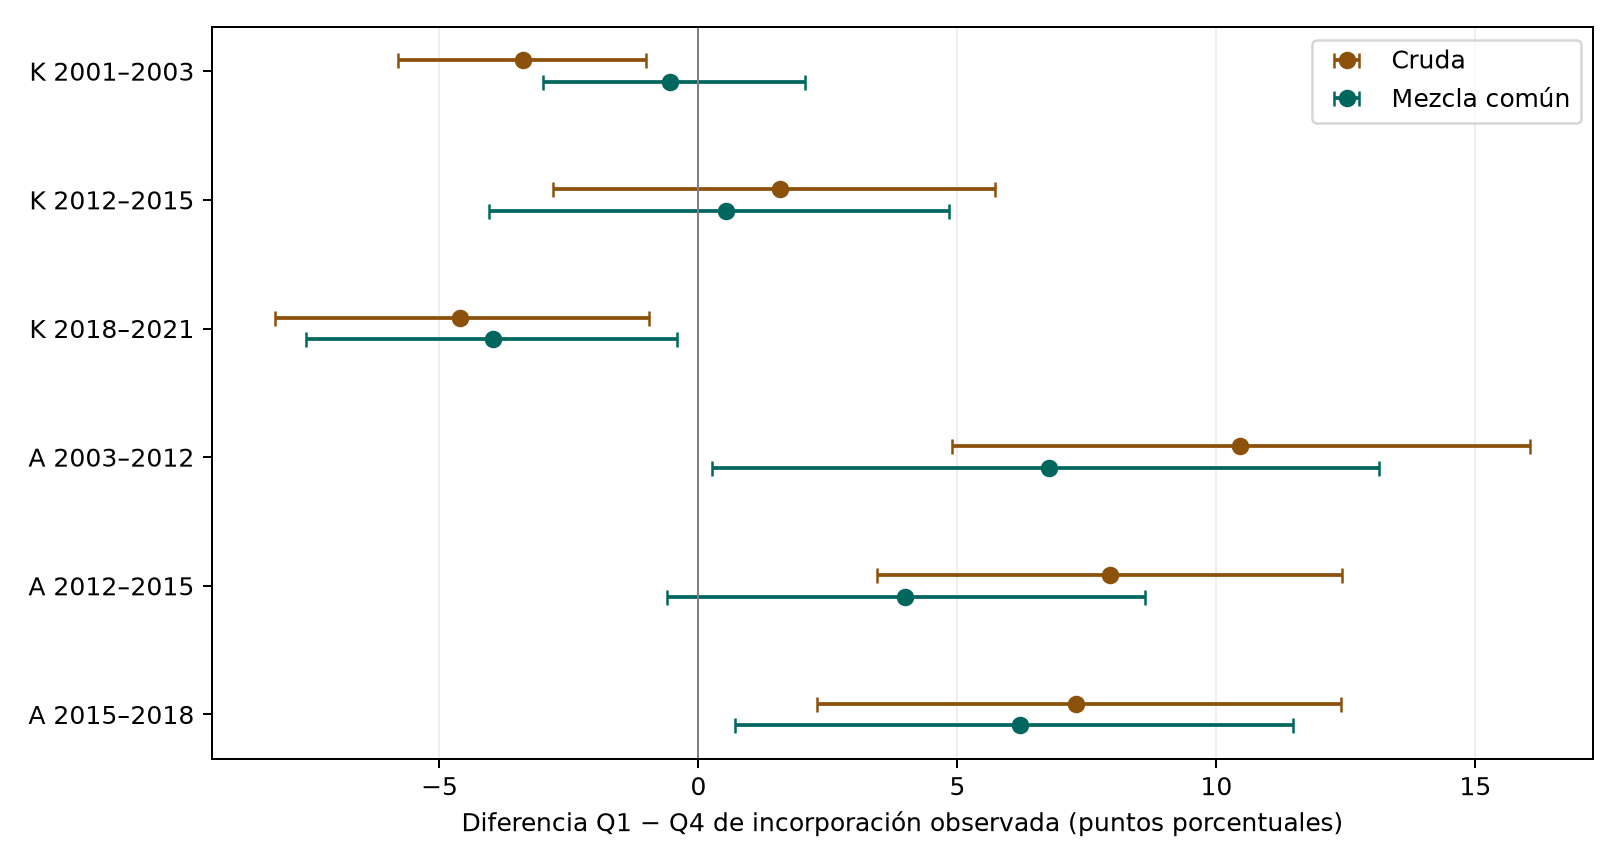
\includegraphics[width=.96\textwidth]{../resultados/figuras/central09_gradiente_patrimonio.png}\caption{Gradiente patrimonial de incorporación e IC95 condicionales por folio. Q1 menos Q4; mezcla común en soporte.}\label{fig:central-gradiente}\end{figure}
La asociación con menor patrimonio no es uniforme. Los gradientes crudos de A son positivos, pero A 2015--2018 incluye cero al cambiar a otra granularidad etaria con soporte adecuado, y A 2012--2015 incluye cero tras ajuste. A 2003--2012 mantiene señal positiva en variantes viables, con seguimiento selectivo. K no reproduce una preferencia uniforme por el menor patrimonio; K 2018--2021 conserva dirección puntual negativa con precisión sensible al soporte. Los cuadros de la sección de calidad del soporte muestran todas las especificaciones, sin elegir por significancia.

Dentro de K 2012--2015, P tiene patrimonio mediano mayor que C y menor que R, no el menor patrimonio de los tres perfiles. P es siete años más joven que C en mediana y tiene dos años más de escolaridad mediana; sus IC de diferencias por folio se conservan en el informe. En A 2015--2018, la diferencia patrimonial P menos C y la de escolaridad incluyen cero; P es seis años más joven. Son contraejemplos frente a equiparar primera vía con mayor necesidad. La localidad se conserva como corte 100 mil, sin llamarlo ruralidad.

\subsection{Importes posteriores y heterogeneidad}
\begingroup
\small\setlength{\tabcolsep}{4pt}
\begin{longtable}{lrrrrr}
\caption{Montos posteriores por protección basal y continuidad}\label{tab:central-montos}\\
\toprule
Vía/ventana & Perfil & N válido & Q25 & Mediana & Q75 \\
\midrule\endfirsthead
\multicolumn{6}{l}{\small Continuación del cuadro \thetable}\\
\toprule
Vía/ventana & Perfil & N válido & Q25 & Mediana & Q75 \\
\midrule\endhead
\bottomrule\endfoot
K 2001--2003 & P & 278 & 3,657.4 & 4,062.5 & 5,626.7 \\
K 2001--2003 & C & 11 & 3,376.0 & 3,376.0 & 6,189.4 \\
K 2001--2003 & R & 1,175 & 3,657.4 & 4,191.9 & 7,196.6 \\
K 2012--2015 & P & 1,060 & 941.5 & 1,027.1 & 3,937.2 \\
K 2012--2015 & C & 373 & 941.5 & 941.5 & 996.3 \\
K 2012--2015 & R & 1,857 & 3,423.6 & 4,279.6 & 10,270.9 \\
K 2018--2021 & P & 360 & 3,859.6 & 4,895.0 & 9,314.1 \\
K 2018--2021 & C & 132 & 2,107.6 & 4,079.2 & 5,234.9 \\
K 2018--2021 & R & 1,954 & 3,859.6 & 5,438.9 & 13,140.5 \\
A 2003--2012 & P & 666 & 962.2 & 962.2 & 1,443.3 \\
A 2003--2012 & C & 98 & 962.2 & 962.2 & 1,034.4 \\
A 2003--2012 & R & 278 & 962.2 & 962.2 & 1,732.0 \\
A 2012--2015 & P & 1,196 & 855.9 & 941.5 & 1,027.1 \\
A 2012--2015 & C & 286 & 855.9 & 941.5 & 1,690.4 \\
A 2012--2015 & R & 723 & 855.9 & 941.5 & 1,140.1 \\
A 2015--2018 & P & 581 & 840.6 & 886.5 & 1,299.2 \\
A 2015--2018 & C & 589 & 840.6 & 886.5 & 1,528.4 \\
A 2015--2018 & R & 1,245 & 840.6 & 886.5 & 1,528.4 \\
\end{longtable}
{\footnotesize Fuente: etapa 09, bases analíticas existentes y eventos originales, muestra no ponderada. P: ambas negativas basales; C: otra vía basal afirmativa; R: continuidad de la vía. No alta administrativa ni inferencia nacional. Pesos mensuales de septiembre de 2026, importe nominal multiplicado por factor del año calendario previo a entrevista real. Suma íntegra solo de eventos captados, no totalidad real. A incluye dinero/especie; no programa homogéneo. Diferencias de captura de la tabla 3.1 se mantienen.\par}
\endgroup

\begingroup\small\setlength{\tabcolsep}{3pt}
\begin{longtable}{lrrrrr}
\caption{Monto posterior por mitad patrimonial y protección basal}\label{tab:central-patrimonio_monto}\\
\toprule
Vía/ventana & Mitad & N P/C & Mediana P & Mediana C & P-C [IC95] \\
\midrule\endfirsthead
\multicolumn{6}{l}{Continuación del cuadro \thetable}\\
\toprule
Vía/ventana & Mitad & N P/C & Mediana P & Mediana C & P-C [IC95] \\
\midrule\endhead
\bottomrule\endfoot
K 2001--2003 & Inferior & Sin soporte & Reservado & Reservado & No estimable \\
K 2001--2003 & Superior & Sin soporte & Reservado & Reservado & No estimable \\
K 2012--2015 & Inferior & 553/230 & 992.9 & 941.5 & 51.4 [8.6; 68.5] \\
K 2012--2015 & Superior & 507/143 & 1,985.7 & 941.5 & 1,044.2 [492.1; 2,482.1] \\
K 2018--2021 & Inferior & 176/71 & 4,740.3 & 4,079.2 & 661.1 [37.7; 1,149.4] \\
K 2018--2021 & Superior & 184/61 & 5,438.9 & 4,079.2 & 1,359.7 [564.7; 2,175.6] \\
A 2003--2012 & Inferior & 372/42 & 962.2 & 962.2 & 0.0 [0.0; 0.0] \\
A 2003--2012 & Superior & 294/56 & 962.2 & 962.2 & 0.0 [0.0; 0.0] \\
A 2012--2015 & Inferior & 661/133 & 941.5 & 941.5 & 0.0 [0.0; 0.0] \\
A 2012--2015 & Superior & 535/153 & 941.5 & 941.5 & 0.0 [-51.4; 0.0] \\
A 2015--2018 & Inferior & 316/321 & 886.5 & 886.5 & 0.0 [-39.7; 7.6] \\
A 2015--2018 & Superior & 265/268 & 878.8 & 886.5 & -7.6 [-38.2; 34.4] \\
\end{longtable}
{\footnotesize Fuente: auditoría10, insumos01--09 intactos. Muestra sin ponderación; IC condicionales, sin inferencia nacional o causal. P: primera vía observada; C: otra vía basal afirmativa. Reformulación común Q1+Q2/Q3+Q4, manteniendo población, titularidad, ventanas y precios. 4999 réplicas por folio. K2001--2003 sigue sin soporte; retirar conjuntamente ambas mitades y derivados impide recuperar un importe mediante otra rama. No se escogió la agrupación por significancia.\par}
\endgroup

\begingroup
\small\setlength{\tabcolsep}{4pt}
\begin{longtable}{lrrrr}
\caption{Diferencia de medianas posteriores: P menos C}\label{tab:central-diferencias}\\
\toprule
Vía/ventana & N P/C & Cruda [IC95] & Mezcla común [IC95] & Retención \% \\
\midrule\endfirsthead
\multicolumn{5}{l}{\small Continuación del cuadro \thetable}\\
\toprule
Vía/ventana & N P/C & Cruda [IC95] & Mezcla común [IC95] & Retención \% \\
\midrule\endhead
\bottomrule\endfoot
K 2001--2003 & 278/11 & No estimado & No estimado & 0/0 \\
K 2012--2015 & 1\,060/373 & 85{,}6 [51{,}4; 409{,}8] & No estimado & 57/90 \\
K 2018--2021 & 360/132 & 815{,}8 [543{,}9; 1\,324{,}3] & No estimado & 20/50 \\
A 2003--2012 & 666/98 & 0{,}0 [0{,}0; 0{,}0] & No estimado & 0/0 \\
A 2012--2015 & 1\,196/286 & 0{,}0 [0{,}0; 0{,}0] & No estimado & 51/79 \\
A 2015--2018 & 581/589 & 0{,}0 [-30{,}6; 7{,}6] & -7{,}6 [-38{,}2; 7{,}6] & 73/89 \\
\end{longtable}
{\footnotesize Fuente: elaboración propia con las bases analíticas y eventos originales de ENASEM; muestra no ponderada. P: ambas negativas basales; C: otra vía basal afirmativa; R: continuidad de la vía. No alta administrativa ni inferencia nacional. Pesos reales. Crudo: bootstrap folio 4999. Mezcla común: sexo por edad de tres grupos por escolaridad 0--5/6+, 1999 réplicas y CDF inversa. Mínimo 20 por grupo/celda, 4 celdas y 70\% de cada grupo completo antes de excluir covariables ND. No estimado si falta soporte; no se extrapola. Crudo y ajustado pueden usar poblaciones y convenciones distintas; crudo del mismo soporte en agregados. Los empates y la concentración de importes pueden producir extremos repetidos o IC de amplitud cero en el bootstrap de medianas; no implican certeza absoluta, igualdad distributiva ni ausencia de incertidumbre.\par}
\endgroup

\begingroup
\small\setlength{\tabcolsep}{4pt}
\begin{longtable}{llrr}
\caption{Heterogeneidad institucional del contraste P menos C}\label{tab:central-instituciones}\\
\toprule
Vía/ventana & Evidencia destino & N P/C & Diferencia real [IC95] \\
\midrule\endfirsthead
\multicolumn{4}{l}{\small Continuación del cuadro \thetable}\\
\toprule
Vía/ventana & Evidencia destino & N P/C & Diferencia real [IC95] \\
\midrule\endhead
\bottomrule\endfoot
K 2012--2015 & IMSS/ISSSTE & 406/27 & 513{,}5 [0{,}0; 984{,}3] \\
K 2012--2015 & Programa agrupado & 599/326 & 0{,}0 [0{,}0; 0{,}0] \\
K 2012--2015 & Un evento IMSS & 305/20 & 428{,}0 [0{,}0; 684{,}7] \\
K 2018--2021 & IMSS/ISSSTE & 309/79 & 679{,}9 [-40{,}0; 1\,087{,}8] \\
K 2018--2021 & Un evento IMSS & 259/68 & 271{,}9 [-193{,}1; 679{,}9] \\
A 2015--2018 & A: INAPAM & 163/155 & -30{,}6 [-45{,}9; 34{,}4] \\
A 2015--2018 & A: Otra institución & 217/257 & 0{,}0 [-7{,}6; 7{,}6] \\
A 2015--2018 & A: PROSPERA & 149/119 & -15{,}3 [-45{,}9; 30{,}6] \\
\end{longtable}
{\footnotesize Fuente: elaboración propia con las bases analíticas y eventos originales de ENASEM; muestra no ponderada. P: ambas negativas basales; C: otra vía basal afirmativa; R: continuidad de la vía. No alta administrativa ni inferencia nacional. IC folio 1999. Evidencia K puede solaparse: no sumar filas ni asignar el importe a cada institución. Un evento exige un solo evento captado; IMSS/ISSSTE no identifica régimen. A solo 2018: nombres reportados, no programa longitudinal homologado ni A5 retrospectivo. Celdas inferiores a 20 no generan IC. Los empates y la concentración de importes pueden producir IC de amplitud cero en el bootstrap de medianas; no implican certeza absoluta, igualdad distributiva ni ausencia de incertidumbre.\par}
\endgroup


\begin{figure}[htbp]\centering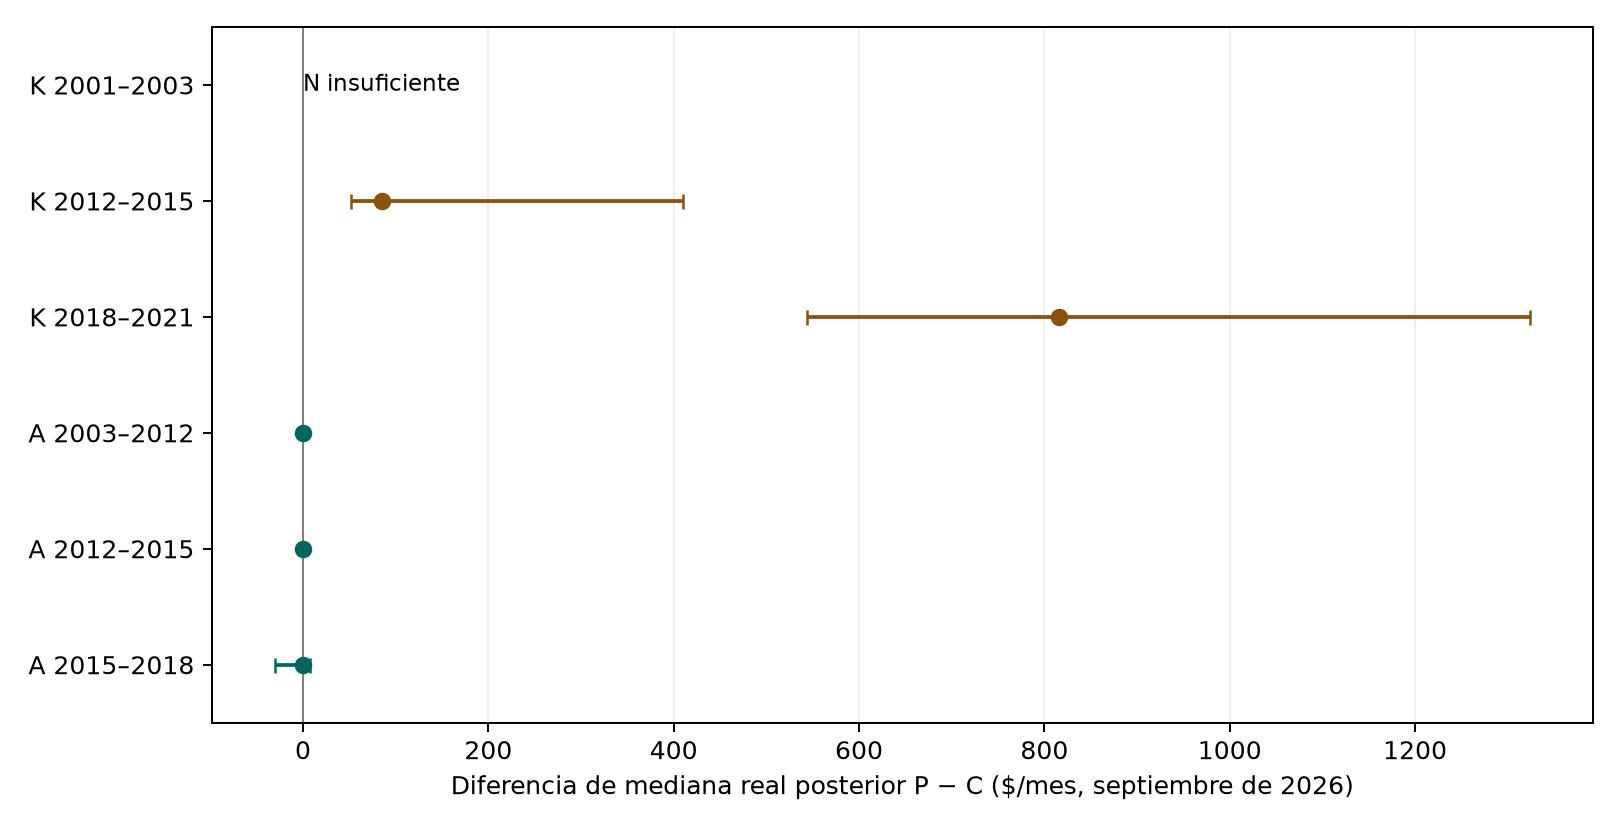
\includegraphics[width=.96\textwidth]{../resultados/figuras/central09_diferencias_montos.png}\caption{Diferencias de medianas posteriores P menos C, pesos mensuales de septiembre de 2026; IC95 por folio.}\label{fig:central-dinero}\end{figure}
En K 2012--2015 y 2018--2021, P tiene una mediana posterior mayor que C; los IC crudos por folio excluyen cero. En 2001--2003 el perfil C solo contiene 12 receptores y 11 montos válidos: se describe, sin IC comparativo. En la definición original, las tres ventanas A comparten la misma mediana P/C en cada destino. Sus IC describen empates, sin demostrar equivalencia económica o distribuciones iguales.

El cuadro~\ref{tab:central-patrimonio_monto}, organizado en mitades patrimoniales, cruza las tres dimensiones de la pregunta: patrimonio inicial, protección previa y monto posterior. No basta con comparar el patrimonio de grupos por un lado y los montos por otro. Los estratos de baja frecuencia se describen sin IC y no se eliminan porque limiten la hipótesis.

La composición importa: en K 2012--2015 el contraste P menos C es mucho mayor entre hombres que entre mujeres y entre 60--64 que entre 70+. Los contrastes por sexo, escolaridad y localidad se sintetizan a continuación; diferencias de intervalos entre estratos no se interpretan como prueba formal de interacción. En A 2015--2018, la estandarización monetaria viable sigue produciendo un contraste cercano a cero. En las restantes ventanas falta soporte para una mediana P/C estandarizada que retenga 70\% de ambos perfiles. No se extrapola el ajuste de nuevos frente a continuos a este contraste diferente.

En la definición original, la evidencia IMSS/ISSSTE atenúa la precisión del contraste P/C en las ventanas K recientes: sus IC incluyen cero. En el código de programas agrupados K 2012--2015 coinciden las medianas. Estas filas pueden solaparse y sus importes no se reparten por institución. Para A solo se desglosan nombres captados al destino 2018 y personas con un evento: ello describe heterogeneidad del destino, sin reconstruir programas previos, A5 o identidad administrativa.

\subsection{Selección, desconocidos y coexistencia}
\begingroup
\small\setlength{\tabcolsep}{4pt}
\begin{longtable}{lrrrrr}
\caption{Seguimiento de cohortes negativas y límites de observación}\label{tab:central-seleccion}\\
\toprule
Vía/ventana & Perfil & N basal & Fallecido & Ausente & Cota \% sin D \\
\midrule\endfirsthead
\multicolumn{6}{l}{\small Continuación del cuadro \thetable}\\
\toprule
Vía/ventana & Perfil & N basal & Fallecido & Ausente & Cota \% sin D \\
\midrule\endhead
\bottomrule\endfoot
K 2001--2003 & P & 4,533 & 239 & 223 & 6.7--19.6 \\
K 2001--2003 & C & 576 & 22 & 22 & 2.2--18.8 \\
K 2012--2015 & P & 4,592 & 319 & 199 & 25.5--35.6 \\
K 2012--2015 & C & 1,323 & 145 & 26 & 31.9--41.7 \\
K 2018--2021 & P & 3,368 & 304 & 184 & 12.5--24.4 \\
K 2018--2021 & C & 2,422 & 337 & 55 & 6.6--19.2 \\
A 2003--2012 & P & 4,368 & 1,165 & 400 & 21.2--46.6 \\
A 2003--2012 & C & 1,631 & 504 & 201 & 8.7--36.8 \\
A 2012--2015 & P & 4,592 & 319 & 199 & 28.3--38.2 \\
A 2012--2015 & C & 2,562 & 214 & 150 & 12.6--23.6 \\
A 2015--2018 & P & 3,253 & 194 & 374 & 19.7--38.1 \\
A 2015--2018 & C & 3,622 & 273 & 382 & 18.1--36.4 \\
\end{longtable}
{\footnotesize Fuente: etapa 09, bases analíticas existentes y eventos originales, muestra no ponderada. P: ambas negativas basales; C: otra vía basal afirmativa; R: continuidad de la vía. No alta administrativa ni inferencia nacional. Cota sin D: entre quienes no tienen fallecimiento registrado, incorporar a todos los destinos no clasificables o a ninguno. No acredita que ausentes estén vivos ni incidencia previa a morir. Fallecimientos quedan separados, sin imputar recepción post mortem. Sustitutos, ND y conflictos separados en informe y agregados.\par}
\endgroup


Las cotas de seguimiento son amplias y no son IC de muestreo: responden a falta de observación, no a la precisión de una mediana entre observados. El informe conserva las particiones exhaustivas de toda cohorte, los perfiles de cada destino, los montos faltantes y las sensibilidades por sustituto, edad final y fecha de precios. Sus resultados no recuperan las trayectorias no observadas. Entre receptores observados, las cotas por importes faltantes mantienen positiva la diferencia mediana P menos C en K 2012--2015 y 2018--2021; no son IC y no incluyen selección de ausentes o fallecidos. Los intervalos exactos permanecen en el informe.

En K 2012--2015, de 376 incorporados con A basal, 130 declaran A al destino, 244 la niegan y 2 son ND. La complementariedad basal no implica acumulación al final: el estado C incluye también pérdida o cambio de declaración de la otra vía, sin acreditar sustitución administrativa.

La otra vía basal no demuestra coexistencia simultánea. El informe tabula afirmativa, negativa y ND de la otra vía al destino para P y C; solo 2012--2015 admite interpretación longitudinal conjunta. En las demás ventanas, esa respuesta de destino es descripción bajo su propio cuestionario. La persistencia sin ambas vías se cuantifica conjuntamente solo donde ambas son comparables. No se interpreta una ruptura como aparición o desaparición económica real.

\subsection{Sensibilidad de la medición y alcance de primera vía}
\label{sec:resultados-sensibilidad-medicion}

Los cuadros~\ref{tab:sensibilidad-medicion-k}--\ref{tab:sensibilidad-ventanas}
conservan la definición original y la alternativa estricta de la
sección~\ref{sec:sensibilidad-medicion}. En K 2012--2015, nuevos receptores
pasan de 1\,469 a 539; P de 1\,090 a 489 y C de 376 a 49. Los demás no se
reclasifican como personas sin recursos, sino como no comparables bajo el
criterio alternativo. En A no cambia la incorporación total, pero sí la
identificación de K basal: C pasa de 296 a 166 en 2012--2015 y de 606 a 153
en 2015--2018. No se demuestra que toda esta diferencia provenga de una
reclasificación real de un mismo programa.

Manteniendo el denominador original de reobservados K, la incorporación
conocida sin 08 es 489/3\,843 entre P, 12{,}72\% (IC95\% por folio:
11{,}69--13{,}84\%), y 49/1\,063 entre C, 4{,}61\% (3{,}32--6{,}00\%).
El orden es opuesto al de la recepción K original, 28{,}36 frente a
35{,}37\%. Se trata de un resultado institucional distinto sobre los mismos
denominadores, no de un efecto de A sobre K ni de una tasa administrativa.
El denominador K no coincide necesariamente con el de unión, porque una
A afirmativa puede resolver esta última aunque K sea desconocida.

En el subgrupo con evidencia IMSS/ISSSTE de destino, apartar solo 08
identificado en las visitas necesarias deja 391/25 montos P/C frente a
406/27 originales. El punto P--C es 513{,}55 en ambos casos; los IC95\%
con 4\,999 réplicas por folio y semilla 20261024 son [171{,}18; 855{,}91]
y [0; 1\,027{,}09], respectivamente. Los C de 25/27 válidos son exploratorios;
no se escoge el intervalo que excluye cero como explicación institucional.
El contraste de un evento IMSS, con 305/20, conserva 427{,}96 [0; 684{,}73].
La rama de un evento ISSSTE no tiene soporte para un contraste. La evidencia
institucional puede ser múltiple y no asigna el importe a una institución.

La diferencia monetaria nuevos menos continuos K pasa de -3\,286{,}70 a
-513{,}55 pesos reales en la alternativa estricta; P menos C pasa de
85{,}59 a 1\,027{,}09. Sus IC y N válidos figuran en el
cuadro~\ref{tab:sensibilidad-medicion-k}. Las magnitudes dependen de la
mezcla institucional. Tener otra vía al inicio no explica causalmente
la diferencia ni acredita un incremento de ingreso total.

La historia previa aporta otro límite: 217 de las 1\,090 personas P de
K 2012--2015 y 148 de las 384 de K 2018--2021 tenían alguna declaración
K/A positiva en una entrevista directa anterior sin conflicto vital. En
A 2012--2015 son 222/1\,210 y en A 2015--2018, 149/603. Esas declaraciones
se leen bajo el cuestionario de cada ronda, sin validar puentes excluidos.
P significa primera vía desde ambas negativas en esa pareja de rondas,
no primera recepción conocida en toda la historia ni de toda la vida.

\paragraph{Patrimonio y magnitud.}
La interacción entre contrastes de mitades patrimoniales K 2012--2015
es 992{,}86 pesos reales, IC95\% [666{,}97; 2\,430{,}79] en la definición
original. Al apartar solo 08 identificado es -684{,}73
[-1\,883{,}01; 3\,595{,}26], con grupos C de 20 y 27 válidos, exploratorios.
El cuadro~\ref{tab:sensibilidad-interaccion} muestra que la heterogeneidad
por patrimonio no es robusta a esta decisión de medición; el signo alternativo
no demuestra una reversión poblacional. Los N de 20 y 27 cuentan personas C
con monto posterior íntegro válido en las mitades basal inferior y superior,
respectivamente; no son frecuencias en la mediana ni números de folios.
El cambio de signo puede reflejar tanto la reclasificación institucional
como la inestabilidad de muestras reducidas; esta sensibilidad no separa
sus contribuciones. No sustenta una conclusión general sobre patrimonio.
En K 2018--2021 la interacción también incluye
cero, aunque los dos contrastes por mitad sean positivos. No basta comparar
sus significancias por separado.

El contraste original K 2012--2015 P--C de 85{,}59 equivale aproximadamente
al 9{,}1\% de la mediana C de 941{,}50; por mitad patrimonial son 5{,}5\% y
110{,}9\%. La precisión no vuelve equivalentes esas magnitudes ni establece
su suficiencia económica. El patrimonio compartido tampoco mide necesidad.

\paragraph{Composición y soporte.}
En K 2012--2015 los N válidos P/C son 478/160 en hombres y 582/213 en
mujeres; los contrastes son 1\,112{,}69 [770{,}32; 2\,482{,}14] y
51{,}35 [8{,}56; 51{,}35]. Con escolaridad basal de cero años,
233/152: 0 [0; 42{,}80]; de 1--5 años, 377/162: 51{,}35 [0; 51{,}35];
con seis años, 249/40: 834{,}51 [34{,}24; 2\,439{,}35]. En localidades
menores de 100 mil habitantes, 486/304: 42{,}80 [17{,}12; 51{,}35]; en las
mayores, 574/69: 2\,054{,}19 [1\,027{,}09; 2\,430{,}79]. Son IC95\%
por folio con 1\,999 réplicas, semilla 20261024, sin ajuste ni prueba formal
de interacción. Los restantes estratos educativos carecen de soporte; no se
utilizan para conclusiones monetarias.

La estandarización monetaria P/C K 2012--2015 no es viable en ninguna de las
cuatro configuraciones de edad y mínimos por celda examinadas. La alternativa
que más se aproxima conserva solo 69{,}72\% de P, por debajo del 70\%
exigido; no se redondea para aceptar el ajuste. El gradiente patrimonial
Q1 menos Q4 de incorporación K, restringido a solo 08 identificado, pasa de
-3{,}95 puntos porcentuales crudos [-7{,}43; -0{,}44] a -1{,}41
[-5{,}08; 2{,}53] al estandarizar sexo, edad y escolaridad, con soporte
749/774 y 1\,999 réplicas, semilla 20261024. La asociación cruda no se
mantiene inequívocamente tras considerar composición.

\paragraph{Atrición e identificación de la unión.}
La fracción detectada original es 2\,188/4\,592, 47{,}65\%; no es una
estimación corregida de incorporación en la cohorte. Excluyendo únicamente
319 defunciones registradas, quedan 4\,273 personas sin esa condición y 427
destinos no clasificables; los límites son 51{,}21--61{,}20\%. No certifican
que los ausentes estén vivos, ni constituyen IC. En la alternativa estricta,
1\,643/3\,301 = 49{,}77\% entre clasificables alternativos; sobre los
3\,846 observados originales se identifica 42{,}72\% y los 545 ND adicionales
permiten límites de medición 42{,}72--56{,}89\%. No hay una única tasa
``corregida'' que reemplace el 56{,}9\% original.

De los 376 incorporados K con A basal, los 130 que conservan A y los 244 que
la niegan incluyen, respectivamente, 109 y 216 con 08 en K. Esto respalda
examinar medición, pero no identifica el beneficio administrativo. Los pares
monetarios válidos A origen/K destino son 127/237, en 117/213 folios. Las
medianas de diferencias reales individuales son -20{,}69 en ambos conjuntos,
IC95\% [-20{,}69; 85{,}65] y [-20{,}69; 22{,}10], con 4\,999 réplicas,
semilla 20261023. A puede incluir especie; esos cambios no son ganancias o
pérdidas del ingreso total ni prueba de continuidad de un programa.


% END central09_resultados
\FloatBarrier
\section*{Contexto descriptivo y contrastes complementarios}
Los resultados siguientes sitúan el contraste central en las seis rondas;
no sustituyen la respuesta sobre incorporación desde negativas basales.

\section{Distribución y superposición de vías propias}
\label{sec:resultados-cobertura}

El cuadro~\ref{tab:tesis-cobertura} distingue recepción propia K, apoyo
propio A y unión de ambas vías entre personas vivas de 60 años o más con
entrevista directa. Cada tasa conserva su denominador conocido y cada
fila corresponde a un corte. Las diferencias de cobertura entre filas que
atraviesan rupturas no se interpretan como una trayectoria homologada.

La selección de ventanas se fundamenta en la
sección~\ref{sec:comparabilidad-ventanas} y el
cuadro~\ref{tab:comparabilidad-ventanas}. Se mantienen los seis cortes
descriptivos incluso donde no se admite transición homologada.
En particular, el cambio A 2018--2021 no estima incorporaciones reales
de una definición invariable; A 2001--2003 mantiene homologación pendiente.

% Exportado desde agregados; no editar cifras manualmente.
\begin{table}[!htbp]
\centering
\caption{Recepción propia y estados de información por ronda, directas 60+, 2001--2021}\label{tab:tesis-cobertura}
\footnotesize\setlength{\tabcolsep}{3pt}\renewcommand{\arraystretch}{1.25}
\begin{tabularx}{\linewidth}{p{.075\linewidth}p{.085\linewidth}YYYp{.135\linewidth}p{.13\linewidth}}
\toprule
\textbf{Ronda} & \textbf{N elegible} & \textbf{K: \% (N)} & \textbf{A: \% (N)} & \textbf{Unión: \% (N)} & \textbf{ND K/A/unión} & \textbf{Ambas negativas} \\
\midrule
2001 & 6\,812 & \ensuremath{24,74}\ \allowbreak\ensuremath{(6\,790)} & \ensuremath{9,81}\ \allowbreak\ensuremath{(6\,789)} & \ensuremath{33,23}\ \allowbreak\ensuremath{(6\,789)} & 22/\allowbreak{}23/\allowbreak{}23 & 4\,533 \\
2003 & 6\,970 & \ensuremath{25,53}\ \allowbreak\ensuremath{(6\,894)} & \ensuremath{12,98}\ \allowbreak\ensuremath{(6\,894)} & \ensuremath{36,64}\ \allowbreak\ensuremath{(6\,894)} & 76/\allowbreak{}76/\allowbreak{}76 & 4\,368 \\
2012 & 8\,888 & \ensuremath{32,26}\ \allowbreak\ensuremath{(8\,738)} & \ensuremath{17,99}\ \allowbreak\ensuremath{(8\,750)} & \ensuremath{47,42}\ \allowbreak\ensuremath{(8\,734)} & 150/\allowbreak{}138/\allowbreak{}154 & 4\,592 \\
2015 & 9\,640 & \ensuremath{43,76}\ \allowbreak\ensuremath{(9\,504)} & \ensuremath{27,65}\ \allowbreak\ensuremath{(9\,513)} & \ensuremath{65,79}\ \allowbreak\ensuremath{(9\,508)} & 136/\allowbreak{}127/\allowbreak{}132 & 3\,253 \\
2018 & 9\,107 & \ensuremath{35,89}\ \allowbreak\ensuremath{(9\,047)} & \ensuremath{30,56}\ \allowbreak\ensuremath{(9\,045)} & \ensuremath{62,74}\ \allowbreak\ensuremath{(9\,039)} & 60/\allowbreak{}62/\allowbreak{}68 & 3\,368 \\
2021 & 9\,424 & \ensuremath{34,82}\ \allowbreak\ensuremath{(9\,366)} & \ensuremath{52,59}\ \allowbreak\ensuremath{(9\,363)} & \ensuremath{67,97}\ \allowbreak\ensuremath{(9\,366)} & 58/\allowbreak{}61/\allowbreak{}58 & 3\,000 \\
\bottomrule
\end{tabularx}
\notacuadro{Cada tasa usa el N conocido entre paréntesis; ND se cuenta sobre el N elegible de la fila y no significa negativa. Unión: alguna afirmativa; no: ambas negativas. K y A se superponen. Las filas son cortes separados, no una serie homogénea a través de rupturas K 2003--2012/K 2015--2018 o A 2001--2003/A 2018--2021.}
\fuentecuadro{Elaboración propia, ENASEM; agregados de notebooks 06--08 y validación focalizada del informe general, secciones 10.2--10.7. Sin ponderación nacional.}
\end{table}

\FloatBarrier

La superposición de K y A implica que sus porcentajes no son aditivos.
Una afirmativa basta para identificar alguna vía propia; clasificar la
combinación exclusiva requiere información adicional. Este criterio explica
que el N de unión conocida pueda exceder el de ambas recepciones conocidas.
En 2021, dentro del grupo de 70 años o más con entrevista directa,
4\,733/5\,099 con unión conocida declaran recepción, 92{,}82\%; el total
es 5\,125, con 26 ND. No es una estimación nacional ni un indicador de
suficiencia económica integral. La información del cónyuge se analiza como contexto y no aumenta la cobertura
propia por asignación automática.

En 2021, \dato{2021.N_KA_si} de \dato{2021.N_KA_conocido} personas con unión
conocida reportan al menos una vía propia (\dato{2021.KA}\%).
Hay \dato{2021.N_KA_no} negativas explícitas de ambas vías y
\dato{2021.N_KA_ND_elegible} estados de unión desconocida entre
\dato{2021.N_elegible} directas elegibles. Son estados diferentes:
las negativas no demuestran ausencia de todos los recursos económicos
y los desconocidos no se añaden a las negativas.

La tipología documentada identifica 538 directas con pareja confirmada y
solo K del cónyuge, con negativas propias K/A; otras 884 tienen negativas
propias y ausencia explícita de pareja residente. Ambos grupos forman parte
de las negativas propias, pero su contexto difiere. En el primero no se
conoce el reparto efectivo del dinero del cónyuge; en el segundo no se
infiere que falte todo apoyo familiar. Esta distinción responde a quiénes
no tienen una vía propia identificada, sin convertirla en clasificación
de pobreza o dependencia económica completa.

\section{Brechas de cobertura por características socioeconómicas}
\label{sec:resultados-perfiles}

Las diferencias de acceso no tienen la misma dirección para todas las vías.
En 2021, la unión es \dato{Perfil.SinEscuela.Union}\% entre quienes no
registran escolaridad (\dato{Perfil.SinEscuela.UnionSi}/\dato{Perfil.SinEscuela.UnionN}),
frente a \dato{Perfil.AltaEscuela.Union}\% con al menos diez años
(\dato{Perfil.AltaEscuela.UnionSi}/\dato{Perfil.AltaEscuela.UnionN}).
No se concluye que el primer grupo tenga mejores recursos:
la comparación monetaria de la sección~\ref{sec:resultados-brechas-monto}
muestra un contraste diferente.

Por edad, la unión pasa de \dato{Perfil.EdadTemprana.Union}\% en 60--64
(\dato{Perfil.EdadTemprana.UnionSi}/\dato{Perfil.EdadTemprana.UnionN})
a \dato{Perfil.EdadMayor.Union}\% en 70+
(\dato{Perfil.EdadMayor.UnionSi}/\dato{Perfil.EdadMayor.UnionN}).
Es una comparación entre perfiles contemporáneos, no un aumento de esa
magnitud al envejecer la misma persona. Las reglas de edad, la generación,
la recepción previa y la supervivencia no se separan causalmente.

En localidades menores de 100 mil habitantes, la unión alcanza
\dato{Perfil.LocalidadMenor.Union}\%
(\dato{Perfil.LocalidadMenor.UnionSi}/\dato{Perfil.LocalidadMenor.UnionN}),
frente a \dato{Perfil.LocalidadMayor.Union}\%
(\dato{Perfil.LocalidadMayor.UnionSi}/\dato{Perfil.LocalidadMayor.UnionN})
en las mayores. El corte no identifica ruralidad estricta y la proximidad
de tasas de unión no prueba igualdad de recursos o necesidades.

La brecha hombre--mujer requiere distinguir el nivel de cada corte del
cambio entre ellos. En 2012--2015, la diferencia de cobertura de unión
se reduce, mientras la diferencia K aislada no presenta un cambio preciso.
Los intervalos y denominadores aparecen conjuntamente con la brecha monetaria
en el cuadro~\ref{tab:tesis-sexo}. La ocupación se mantiene como perfil
descriptivo en los agregados: no se interpreta retirado/incapacitado/no
trabaja como una categoría homogénea de pensionados ni se añade un modelo
laboral explicativo.

\section{Evolución de montos nominales y reales}
\label{sec:resultados-montos}

El cuadro~\ref{tab:tesis-montos} conserva el nivel nominal y el poder
adquisitivo común de los importes captados. El número de receptoras y
receptores es mayor que el N con monto válido. Los cuantiles de los
cortes responden a sus distribuciones disponibles y no a un panel de
beneficiarios fijos.

% Exportado desde agregados; no editar cifras manualmente.
\begin{table}[!htbp]
\centering
\caption{Montos mensuales captados y referencia económica, directas 60+, 2001--2021}\label{tab:tesis-montos}
\footnotesize\setlength{\tabcolsep}{3pt}\renewcommand{\arraystretch}{1.25}
\begin{tabularx}{\linewidth}{p{.075\linewidth}p{.04\linewidth}YYYYY}
\toprule
\textbf{Ronda} & \textbf{Vía} & \textbf{N recibe} & \textbf{N nom./real} & \textbf{Mediana nominal (\$)} & \textbf{Mediana real (\$)} & \textbf{Prestación/ LPI: mediana \% (N)} \\
\midrule
2001 & K & 1\,680 & 1\,608/\allowbreak{}1\,608 & 1\,227,00 & 3\,856,54 & 80,38 (1\,170) \\
2003 & K & 1\,760 & 1\,714/\allowbreak{}1\,714 & 1\,490,00 & 4\,191,92 & 86,62 (1\,247) \\
2012 & K & 2\,819 & 2\,633/\allowbreak{}2\,633 & 2\,200,00 & 4\,233,66 & 92,84 (2\,632) \\
2015 & K & 4\,159 & 3\,965/\allowbreak{}3\,965 & 2\,200,00 & 3\,766,01 & 78,22 (3\,963) \\
2018 & K & 3\,247 & 2\,994/\allowbreak{}2\,994 & 2\,800,00 & 4\,279,56 & 95,58 (2\,994) \\
2021 & K & 3\,261 & 3\,062/\allowbreak{}3\,062 & 4\,000,00 & 5\,438,89 & 119,49 (3\,062) \\
2001 & A & 666 & 625/\allowbreak{}625 & 200,00 & 628,61 & 20,39 (81) \\
2003 & A & 895 & 821/\allowbreak{}821 & 250,00 & 703,34 & 28,87 (142) \\
2012 & A & 1\,574 & 1\,535/\allowbreak{}1\,534 & 500,00 & 962,20 & 24,09 (1\,533) \\
2015 & A & 2\,630 & 2\,582/\allowbreak{}2\,582 & 550,00 & 941,50 & 20,76 (2\,582) \\
2018 & A & 2\,764 & 2\,699/\allowbreak{}2\,699 & 580,00 & 886,48 & 20,47 (2\,699) \\
2021 & A & 4\,924 & 4\,883/\allowbreak{}4\,883 & 1\,550,00 & 2\,107,57 & 43,66 (4\,883) \\
2021 & A5 & 4\,784 & 4\,758/\allowbreak{}4\,758 & 1\,550,00 & 2\,107,57 & 43,66 (4\,758) \\
\bottomrule
\end{tabularx}
\notacuadro{K/A: suma personal observada parcial, no ingreso total. A5: evento explícito de vejez; no se añade de nuevo a A. Pesos reales de septiembre de 2026, precios del año calendario anterior a entrevista real. LPI por persona/mes del mismo periodo: la razón se calcula individualmente antes de resumir. En 2001/2003 solo localidades de al menos 100 mil habitantes tienen ámbito asignable; su N de LPI no es comparable con el total posterior. Una prestación bajo LPI no clasifica pobreza.}
\fuentecuadro{Elaboración propia, ENASEM; agregados de notebooks 06--08 y validación focalizada del informe general, secciones 10.2--10.7. Sin ponderación nacional.}
\end{table}

\FloatBarrier

En K 2012--2015, las medianas nominales son
\$\dato{K.2012.Nominal} y \$\dato{K.2015.Nominal}; las reales pasan de
\$\dato{K.2012.Real} a \$\dato{K.2015.Real}, con
\dato{K.2012.N}/\dato{K.2015.N} importes válidos.
El nivel nominal central sin aumento no mantiene su poder adquisitivo.
La igualdad nominal de 2\,200 pesos no implica igualdad distributiva:
Q25/Q75 son 1\,800/5\,000 en 2012 y 600/4\,000 en 2015. La diferencia
de medianas reales entre cortes es -467{,}65, IC95\% [-467{,}65; -275{,}21],
con 2\,633/3\,965 montos válidos, 4\,836 personas y 4\,225 folios.
Se usan 4\,999 réplicas conjuntas por folio, semilla 20261024;
no es una pérdida de las mismas personas.
Al mismo tiempo, el cuadro~\ref{tab:tesis-cobertura} muestra más recepción K.
Esta coexistencia es compatible con H1 en esa ventana; no identifica
qué parte del cambio se debe a cada componente de la mezcla de receptores.

En A 2015--2018, la mediana nominal pasa de
\$\dato{A.2015.Nominal} a \$\dato{A.2018.Nominal}, pero la real cambia de
\$\dato{A.2015.Real} a \$\dato{A.2018.Real}, con
\dato{A.2015.N}/\dato{A.2018.N} montos válidos.
La diferencia de medianas reales entre estos cortes A es -55{,}02,
IC95\% [-55{,}02; -55{,}02], con 2\,582/2\,699 válidos, 4\,041 personas y
3\,341 folios; 4\,999 réplicas conjuntas, semilla 20261024. La degeneración
del IC refleja acumulaciones de importes, no ausencia de incertidumbre de
medición o selección. La recepción A aumenta en una ventana con
comparabilidad condicionada.
El incremento de pesos declarados no constituye una mejora real de la
mediana. A incluye dinero y especie y cambia su captación por eventos;
no se atribuye todo el patrón a una prestación federal.

\begin{landscape}
\begin{figure}[p]
\centering
\caption{Cobertura y poder adquisitivo en las ventanas K 2012--2015 y A 2015--2018}
\label{fig:tesis-cobertura-monto}
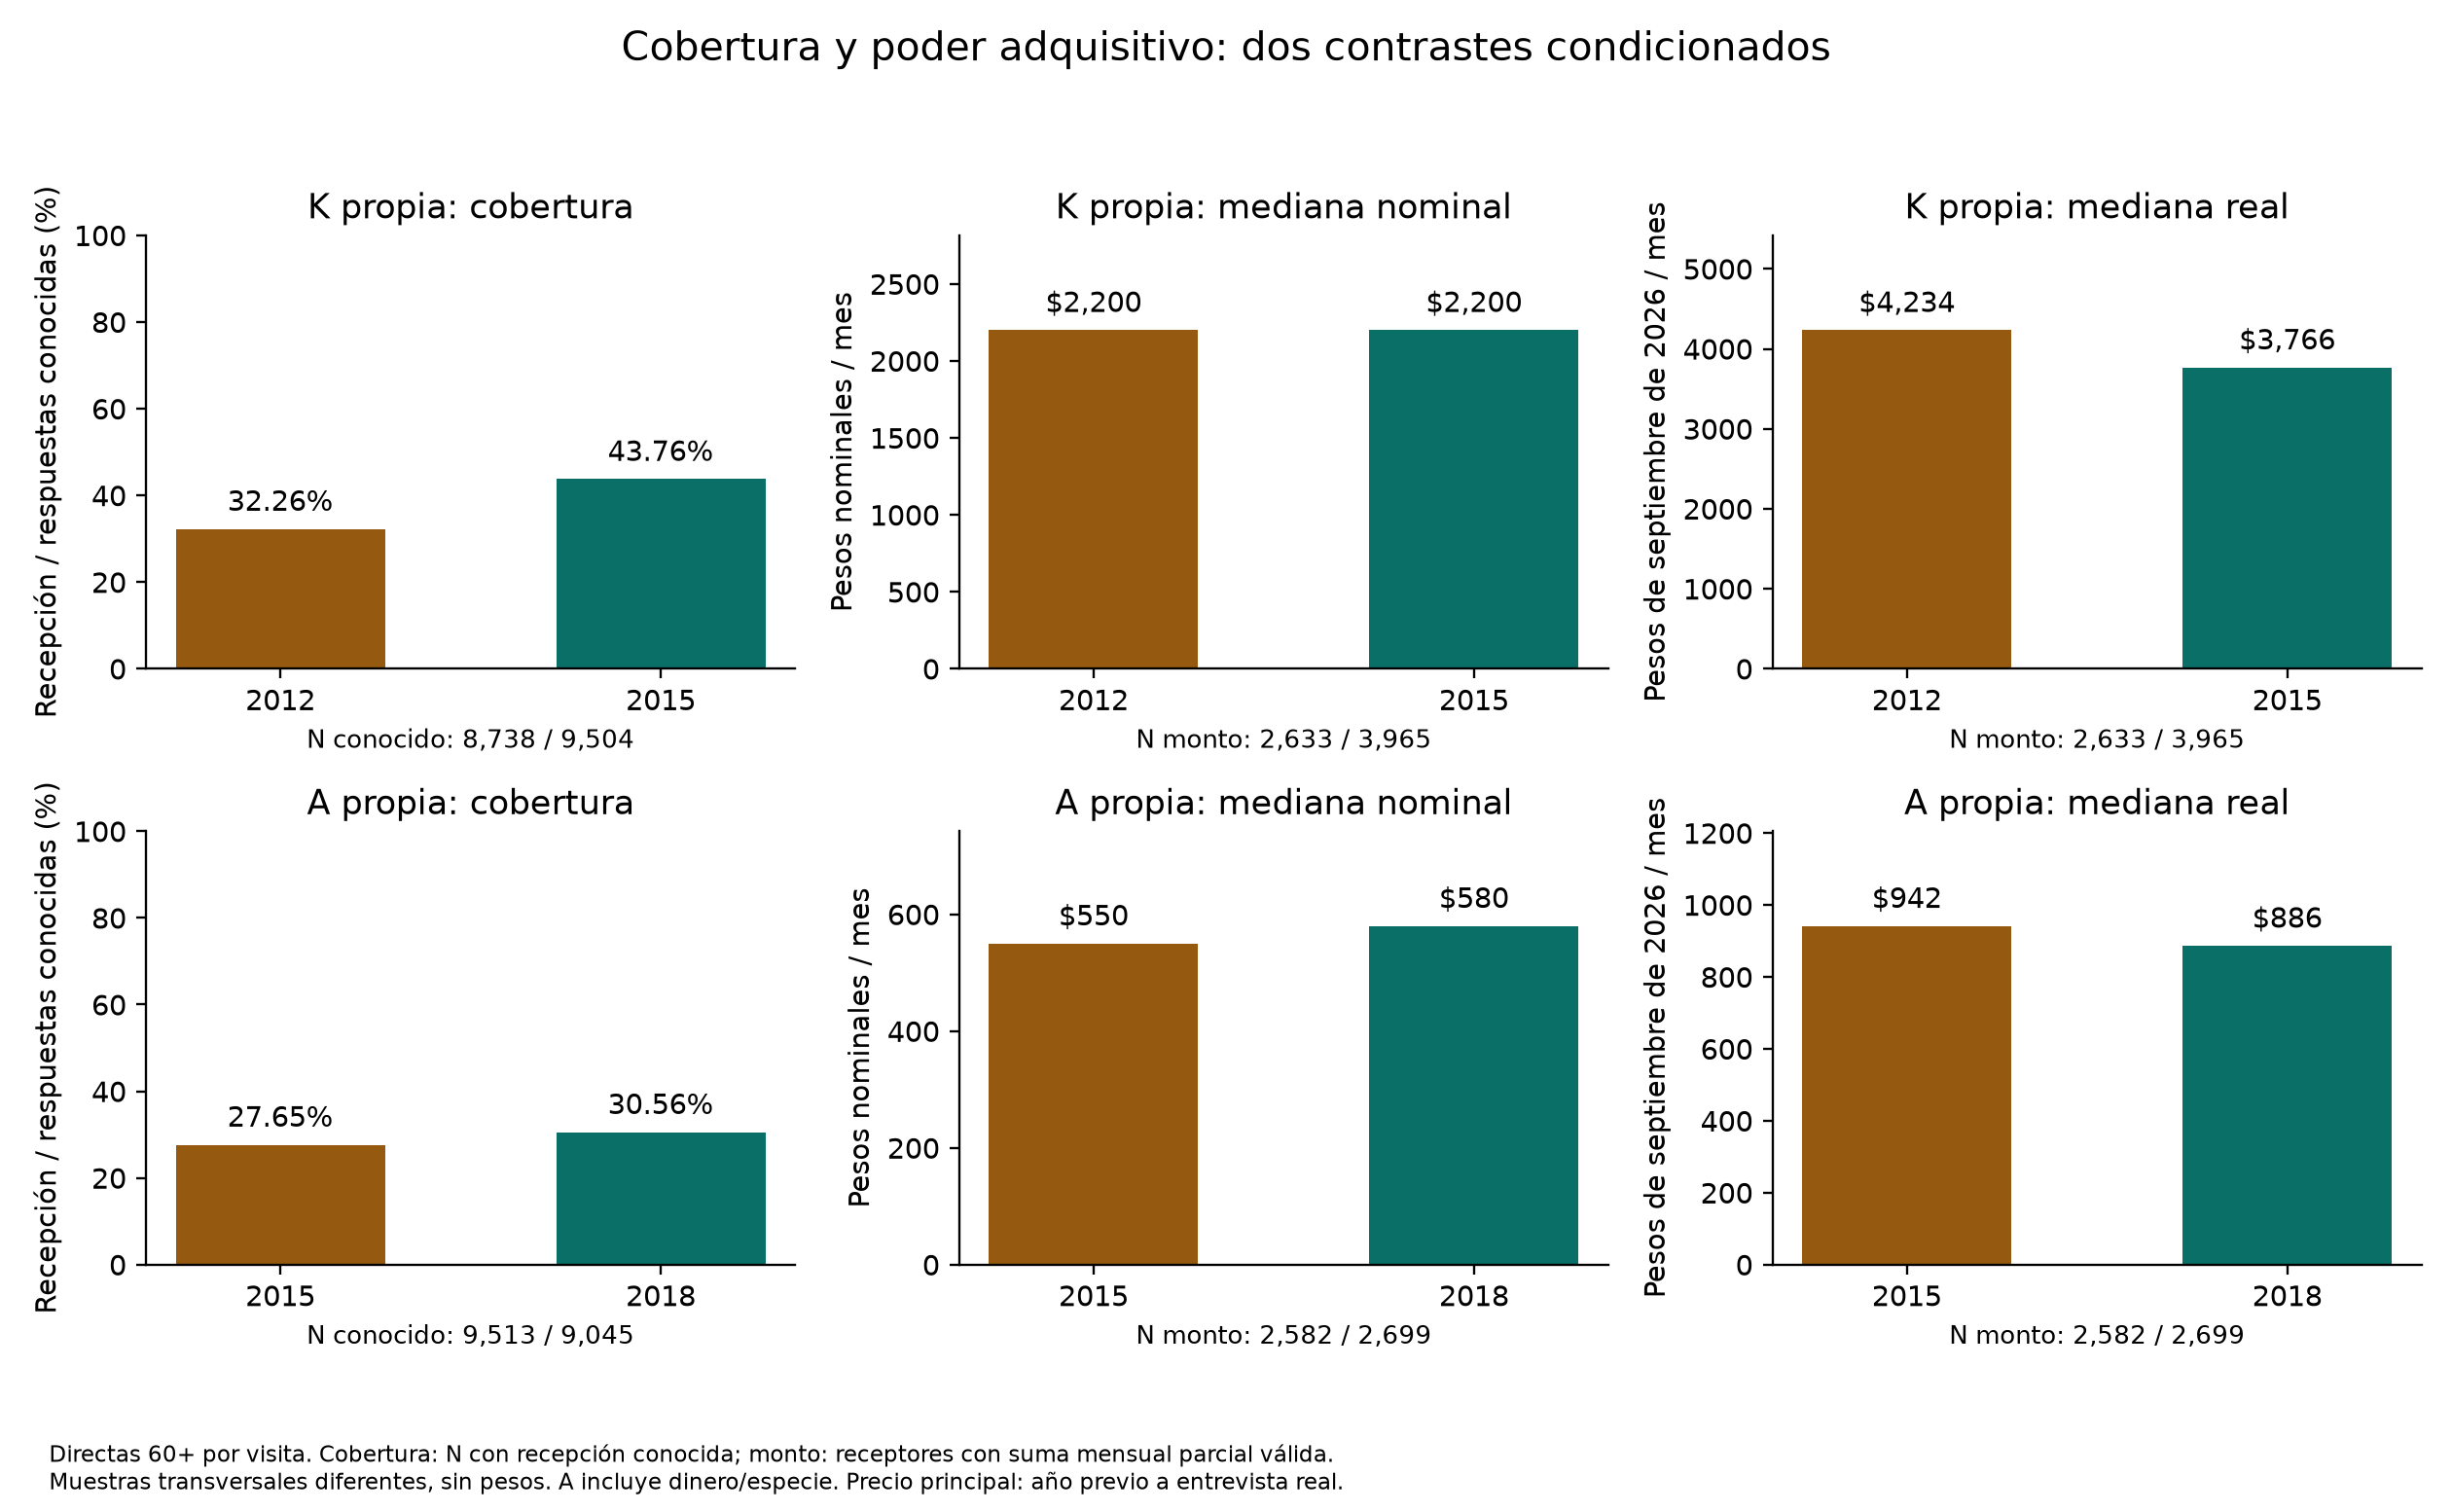
\includegraphics[width=\linewidth,height=.72\textheight,keepaspectratio]{../resultados/figuras/sintesis_proteccion__cobertura_poder_adquisitivo.png}
\notacuadro{Directas 60+ de cada visita; tasas entre respuestas conocidas y montos entre receptores con suma parcial válida. Las escalas nominales y reales están separadas. La figura compara cortes, no cambios individuales; N en los cuadros~\ref{tab:tesis-cobertura} y~\ref{tab:tesis-montos}.}
\fuentecuadro{Elaboración propia, síntesis de agregados de recepción y montos e Informe General, figura 44. Valores reales de septiembre de 2026.}
\end{figure}
\end{landscape}
\FloatBarrier

El patrón no es uniforme: entre 2018 y 2021 la mediana real K aumenta de
\$\dato{K.2018.Real} a \$\dato{K.2021.Real}, con
\dato{K.2018.N}/\dato{K.2021.N} montos válidos, mientras su tasa de recepción
desciende ligeramente. Es un contraejemplo pertinente frente a una lectura
de erosión universal. No autoriza atribuir el aumento real a Bienestar:
K no identifica ese programa y A 2018--2021 presenta una ruptura.

\section{Brechas monetarias y referencia de suficiencia}
\label{sec:resultados-brechas-monto}

La mayor recepción de unión entre personas sin escolaridad coexiste con
una mediana K de \$\dato{Perfil.SinEscuela.Nominal} nominales y
\$\dato{Perfil.SinEscuela.Real} reales (N=\dato{Perfil.SinEscuela.MontoN}),
frente a \$\dato{Perfil.AltaEscuela.Nominal} y
\$\dato{Perfil.AltaEscuela.Real} con al menos diez años
(N=\dato{Perfil.AltaEscuela.MontoN}). Los N monetarios son subconjuntos de
receptores y no los N de cobertura. La diferencia grande documenta
heterogeneidad económica, sin identificar un efecto de la escolaridad.

En localidades menores de 100 mil, la mediana K real es
\$\dato{Perfil.LocalidadMenor.Real} (N=\dato{Perfil.LocalidadMenor.MontoN});
en las mayores, \$\dato{Perfil.LocalidadMayor.Real}
(N=\dato{Perfil.LocalidadMayor.MontoN}). Los importes nominales son
\$\dato{Perfil.LocalidadMenor.Nominal} y
\$\dato{Perfil.LocalidadMayor.Nominal}. Tasas de unión relativamente próximas
pueden coexistir con niveles monetarios diferentes. No se ajustan conjuntamente
historia laboral, instituciones y cohorte en este contraste.

% Exportado desde agregados; no editar cifras manualmente.
\begin{table}[!htbp]
\centering
\caption{Brechas hombre--mujer y cambio de brecha, directas 60+, 2012--2015}\label{tab:tesis-sexo}
\footnotesize\setlength{\tabcolsep}{3pt}\renewcommand{\arraystretch}{1.25}
\begin{tabularx}{\linewidth}{YYYY}
\toprule
\textbf{Indicador y unidad} & \textbf{Brecha2012 [IC95\%]} & \textbf{Brecha2015 [IC95\%]} & \textbf{Cambio2015--2012 [IC95\%]} \\
\midrule
Cobertura K (pp) & \ensuremath{14,79}\ \allowbreak\ensuremath{[12,84;\,16,74]} & \ensuremath{15,27}\ \allowbreak\ensuremath{[13,25;\,17,20]} & \ensuremath{0,47}\ \allowbreak\ensuremath{[-1,73;\,2,60]} \\
Cobertura unión K/A (pp) & \ensuremath{12,43}\ \allowbreak\ensuremath{[10,35;\,14,54]} & \ensuremath{9,24}\ \allowbreak\ensuremath{[7,33;\,11,11]} & \ensuremath{-3,19}\ \allowbreak\ensuremath{[-5,62;\,-0,84]} \\
Mediana K nominal (pesos/mes) & \ensuremath{262,00}\ \allowbreak\ensuremath{[200,00;\,400,00]} & \ensuremath{400,00}\ \allowbreak\ensuremath{[300,00;\,400,00]} & \ensuremath{138,00}\ \allowbreak\ensuremath{[0,00;\,200,00]} \\
Mediana K real (pesos/mes) & \ensuremath{504,19}\ \allowbreak\ensuremath{[384,88;\,769,76]} & \ensuremath{684,73}\ \allowbreak\ensuremath{[513,55;\,684,73]} & \ensuremath{180,54}\ \allowbreak\ensuremath{[-85,03;\,299,85]} \\
\bottomrule
\end{tabularx}
\notacuadro{Cobertura K: N conocidos H/M en2012=3\,996/4\,742 y 2015=4\,229/5\,275; unión: 3\,995/4\,739 y 4\,229/5\,279. Montos K parciales: 1\,485/1\,148 y 2\,085/1\,880 entre receptores. Elegibles por corte: 8\,888/9\,640; ND no es negativa. Bootstrap conjunto de 11\,168 IDs (18\,528 personas-ronda), con todas sus visitas. IC puntuales condicionales; pesos reales de septiembre de 2026. El cambio de brecha entre cortes no es cambio individual.}
\fuentecuadro{Elaboración propia, ENASEM; agregados de notebooks 06--08 y validación focalizada del informe general, secciones 10.2--10.7. Sin ponderación nacional.}
\end{table}

\FloatBarrier

En 2012--2015, el cambio de brecha de unión hombre--mujer es
\dato{Sexo.Union.IC} puntos porcentuales: el IC está por debajo de cero.
Para K aislada, \dato{Sexo.K.IC} no establece dirección de cambio.
La diferencia monetaria K es positiva en los dos cortes, pero su cambio real
\dato{Sexo.Monto.IC} incluye cero. Por tanto, la evidencia apoya una reducción
del contraste de acceso de unión sin acreditar un cierre monetario.
El aumento puntual de la brecha de dinero no debe describirse como
ensanchamiento estadísticamente establecido. La sensibilidad con suma
íntegra conserva las medianas y el mismo diagnóstico.

Para A5/2021 hay \dato{A5.N} personas/eventos explícitos y
\dato{A5.Valido} importes válidos. La mediana es \$\dato{A5.Nominal}
nominales y \$\dato{A5.Real} reales; la mediana de la razón prestación/LPI
es \dato{A5.LPI}\%. La referencia muestra que esa prestación central es
una fracción del umbral mensual por persona. No permite clasificar como
pobres a los receptores ni afirmar que carecen de otros ingresos. La
comparación con importes normativos distingue periodo de recuerdo y fecha
de entrevista: una coincidencia o discrepancia no demuestra cumplimiento,
pago omitido o identificación de programa.

\section{Nuevos receptores frente a continuos}

La comparación K 2012--2015 conserva el cambio de espacios de captación
y la evidencia institucional múltiple; A 2015--2018 conserva el paso de
donativo agregado a eventos. Las diferencias monetarias se refieren
a lo captado bajo esas condiciones, no a una misma prestación administrativa
ni a un efecto de reforma (cuadro~\ref{tab:comparabilidad-ventanas}).
\label{sec:resultados-incorporacion}

Las cohortes basales principales son \dato{K.Basal} para K 2012--2015 y
\dato{A.Basal} para A 2015--2018. Entre ellas,
\dato{K.Conocidos}/\dato{A.Conocidos} tienen pares de recepción conocida,
respectivamente. El contraste de montos de destino utiliza un subconjunto:
nuevos K \dato{K.Nuevo.N}/\dato{K.Nuevo.Recepcion} y continuos K
\dato{K.Continuo.N}/\dato{K.Continuo.Recepcion}; nuevos A
\dato{A.Nuevo.N}/\dato{A.Nuevo.Recepcion} y continuos A
\dato{A.Continuo.N}/\dato{A.Continuo.Recepcion}.
Los faltantes monetarios correspondientes son
\dato{K.Nuevo.Faltantes}/\dato{K.Continuo.Faltantes} en K y
\dato{A.Nuevo.Faltantes}/\dato{A.Continuo.Faltantes} en A.

% Exportado desde agregados; no editar cifras manualmente.
\begin{table}[!htbp]
\centering
\caption{Nuevos menos continuos: diferencias de medianas mensuales en K 2012--2015 y A 2015--2018}\label{tab:tesis-incorporacion}
\footnotesize\setlength{\tabcolsep}{3pt}\renewcommand{\arraystretch}{1.25}
\begin{tabularx}{\linewidth}{YYYY}
\toprule
\textbf{Vía y comparación} & \textbf{N nuevos/continuos} & \textbf{Nominal [IC95\%]} & \textbf{Real [IC95\%]} \\
\midrule
K 2012--15: crudo & 1\,435/1\,857 & \ensuremath{-1\,920,00}\ \allowbreak\ensuremath{[-2\,020,00;\,-1\,870,00]} & \ensuremath{-3\,286,70}\ \allowbreak\ensuremath{[-3\,457,88;\,-3\,201,11]} \\
K: composición común & 1\,428/1\,846 & \ensuremath{-1\,820,00}\ \allowbreak\ensuremath{[-1\,920,00;\,-1\,800,00]} & \ensuremath{-3\,115,52}\ \allowbreak\ensuremath{[-3\,286,70;\,-3\,081,28]} \\
K: evidencia IMSS/ISSSTE & 433/1\,671 & \ensuremath{0,00}\ \allowbreak\ensuremath{[-150,00;\,100,00]} & \ensuremath{0,00}\ \allowbreak\ensuremath{[-256,77;\,171,18]} \\
A 2015--18: crudo & 1\,173/1\,245 & \ensuremath{0,00}\ \allowbreak\ensuremath{[-5,00;\,0,00]} & \ensuremath{0,00}\ \allowbreak\ensuremath{[-7,64;\,0,00]} \\
A: composición común & 1\,087/1\,192 & \ensuremath{0,00}\ \allowbreak\ensuremath{[-5,00;\,0,00]} & \ensuremath{0,00}\ \allowbreak\ensuremath{[-7,64;\,0,00]} \\
\bottomrule
\end{tabularx}
\notacuadro{Directas 60+ basales, destino directo y recepción conocida en ambas visitas; montos íntegros entre eventos captados en destino. IC percentiles por persona, 9,999 réplicas. Composición común: sexo, edad y escolaridad basales, soporte fijo, cuantiles de CDF. Evidencia IMSS/ISSSTE puede coexistir con otras instituciones: no reparte el importe ni identifica régimen. Pesos reales de septiembre de 2026; no IC de diseño.}
\fuentecuadro{Elaboración propia, ENASEM; agregados de notebooks 06--08 y validación focalizada del informe general, secciones 10.2--10.7. Sin ponderación nacional.}
\end{table}

\FloatBarrier

En K, las medianas de destino de nuevos y continuos son
\$\dato{K.Nuevo.nominal}/\$\dato{K.Continuo.nominal} nominales y
\$\dato{K.Nuevo.real}/\$\dato{K.Continuo.real} reales.
En la definición original, la diferencia real \dato{K.Contraste.IC} es grande frente a los niveles
comparados. La diferencia ajustada a composición basal común,
\dato{K.Ajustado.IC}, sigue siendo negativa. No basta igualar sexo, edad y escolaridad observados para eliminar el
contraste original; ello no lo vuelve robusto a cambios de definición
institucional, como muestra el cuadro~\ref{tab:sensibilidad-medicion-k}.

En A, ambos grupos tienen mediana nominal
\$\dato{A.Nuevo.nominal} y real \$\dato{A.Nuevo.real}.
La diferencia \dato{A.Contraste.IC} y la ajustada
\dato{A.Ajustado.IC} incluyen cero. El centro registrado es parecido;
no se demuestra equivalencia distributiva. La distribución A tiene
acumulación de importes y diferencias de colas cuya precisión no ofrece
la misma conclusión que el gran contraste K.

\begin{landscape}
\begin{figure}[p]
\centering
\caption{Distribuciones monetarias de nuevos y continuos en las dos ventanas centrales}
\label{fig:tesis-incorporacion}
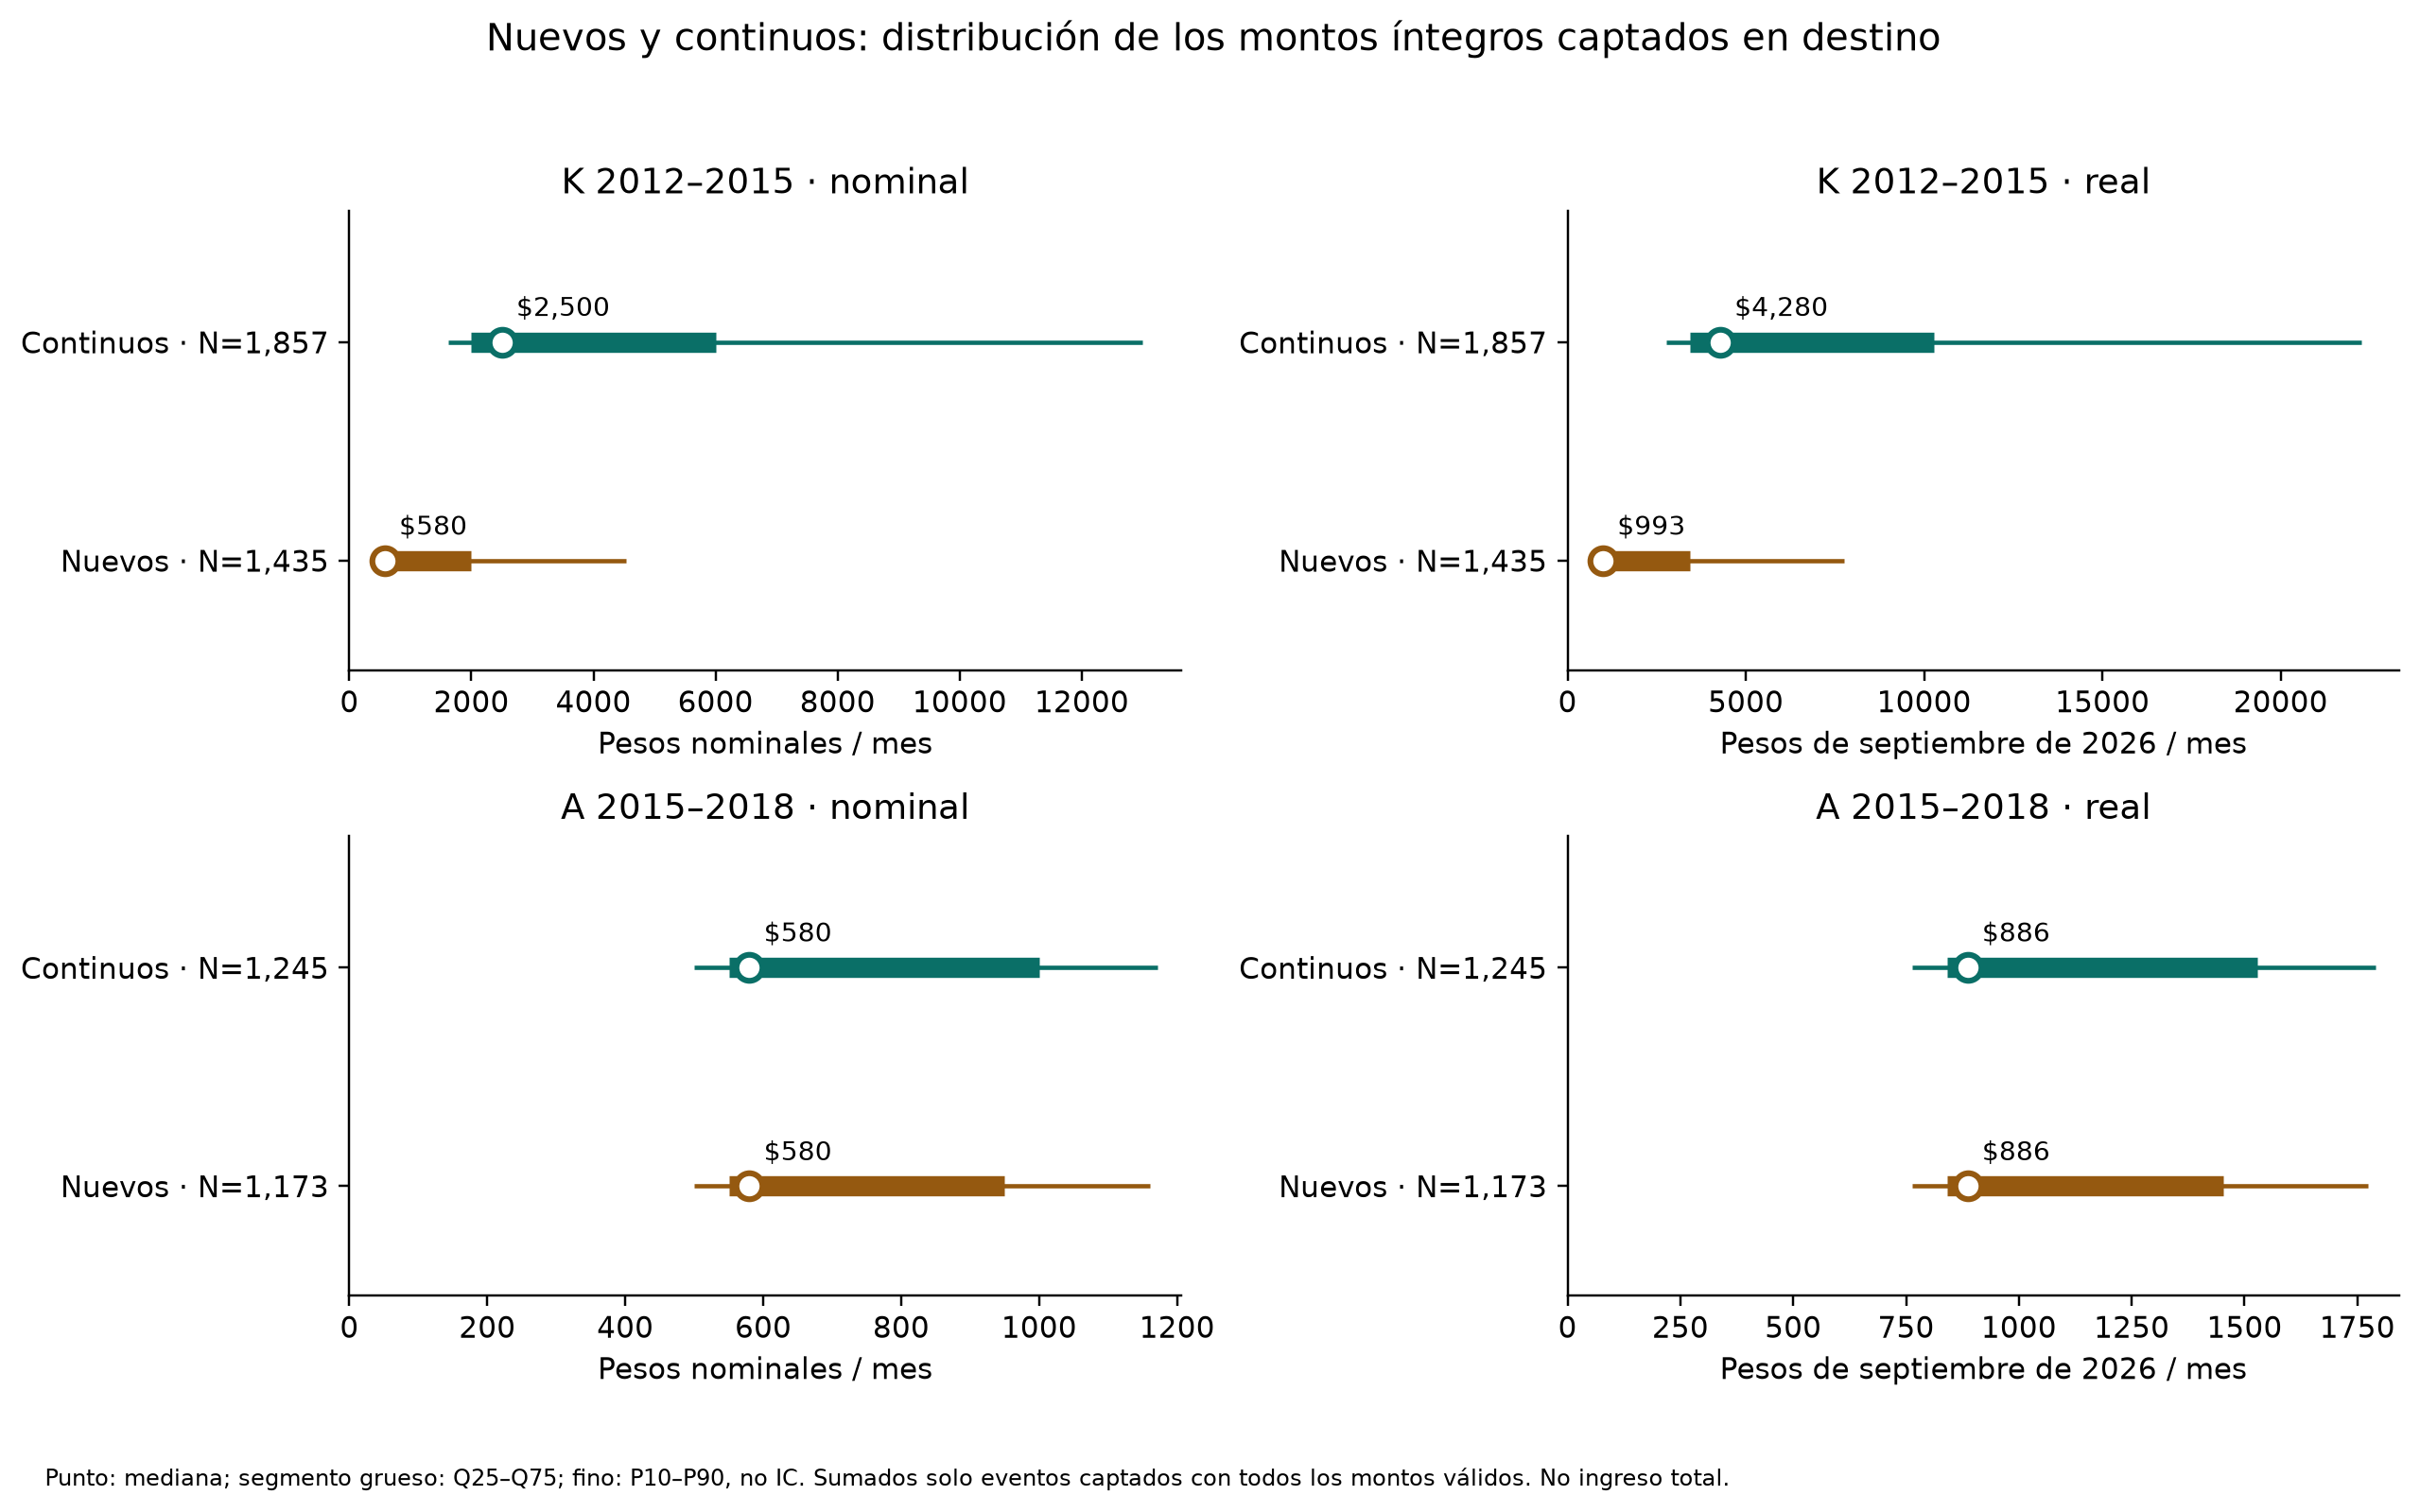
\includegraphics[width=\linewidth,height=.72\textheight,keepaspectratio]{../resultados/figuras/transiciones_montos__nuevos_continuos.png}
\notacuadro{Montos mensuales de destino íntegros entre eventos captados; nuevas respuestas afirmativas y continuidad observadas. N y faltantes en el texto y cuadro~\ref{tab:tesis-incorporacion}. Cuantiles describen dispersión y no sustituyen IC. Comparación K 2012--2015 y A 2015--2018, no una prueba entre programas homogéneos.}
\fuentecuadro{Elaboración propia, agregados longitudinales; Informe General, figura 46. Nominales y pesos de septiembre de 2026.}
\end{figure}
\end{landscape}
\FloatBarrier

Como se documentó en la sección~\ref{sec:resultados-complementariedad},
la incorporación a K o A puede registrarse en quien ya declaraba la otra,
sin acreditar una prestación económica adicional.
La comparación monetaria nuevos--continuos no separa en sí misma los
importes según ese estado basal de complementariedad.

\section{Heterogeneidad institucional}

Con evidencia IMSS/ISSSTE, los nuevos y continuos K tienen ambas medianas
nominales de 2\,500 pesos; el contraste real es
\dato{K.Institucional.IC}, cuyo intervalo incluye cero.
La diferencia entre el contraste total y el del subgrupo solapado es
\dato{K.DiferenciaContrastes.IC}. El remuestreo utiliza las mismas personas
en ambas cantidades, respetando su solapamiento.

La lectura institucional no consiste en que el total K y ese subgrupo
representen regímenes excluyentes. La evidencia puede ser múltiple y el
importe es personal, no separable por institución. El código agrupado8
aparece en 927/1\,435 nuevos con monto y 144/1\,857 continuos.
Esa diferencia acompaña una mezcla institucional distinta, pero no identifica
por sí sola PAM, contributividad o la fracción de una caída atribuible
a política pública.

El contraste grande del conjunto y la coincidencia mediana del subgrupo
limitan una explicación uniforme sobre los receptores K. No prueban que
la institución cause un nivel monetario ni que todos sus miembros tengan
distribuciones iguales. La hipótesis sobre composición gana una descripción
más específica, no una descomposición causal del cambio transversal.

\section{Cambios individuales frente a diferencias transversales}
\label{sec:resultados-cambios}

El cuadro~\ref{tab:tesis-cambios} utiliza \dato{K.Pares} pares K y
\dato{A.Pares} A con importes íntegros captados en ambas visitas.
Son las mismas personas dentro de cada fila. El cambio expresa diferencia
en el monto mensual entre visitas, no una pérdida mensual recurrente ni
una tasa anual.

% Exportado desde agregados; no editar cifras manualmente.
\begin{table}[!htbp]
\centering
\caption{Mediana del cambio real individual entre receptores continuos}\label{tab:tesis-cambios}
\footnotesize\setlength{\tabcolsep}{3pt}\renewcommand{\arraystretch}{1.25}
\begin{tabularx}{\linewidth}{YYYYY}
\toprule
\textbf{Vía y periodo} & \textbf{Criterio} & \textbf{N pares} & \textbf{$\Delta$ [IC95\%]} & \textbf{Por folio [IC95\%]} \\
\midrule
K 2012--2015 & Periodo principal & 1\,756 & \ensuremath{-40,26}\ \allowbreak\ensuremath{[-82,77;\,-19,00]} & \ensuremath{-40,26}\ \allowbreak\ensuremath{[-82,77;\,-19,00]} \\
K 2012--2015 & Doce meses previos & 1\,756 & \ensuremath{-13,59}\ \allowbreak\ensuremath{[-40,84;\,24,75]} & \ensuremath{-13,59}\ \allowbreak\ensuremath{[-40,84;\,24,75]} \\
K 2012--2015 & Año de entrevista & 1\,756 & \ensuremath{5,86}\ \allowbreak\ensuremath{[-30,52;\,34,03]} & \ensuremath{5,86}\ \allowbreak\ensuremath{[-30,52;\,34,03]} \\
A 2015--2018 & Periodo principal & 1\,223 & \ensuremath{-55,02}\ \allowbreak\ensuremath{[-55,02;\,-33,63]} & \ensuremath{-55,02}\ \allowbreak\ensuremath{[-55,02;\,-30,57]} \\
A 2015--2018 & Doce meses previos & 1\,223 & \ensuremath{-68,17}\ \allowbreak\ensuremath{[-72,39;\,-57,79]} & \ensuremath{-68,17}\ \allowbreak\ensuremath{[-73,32;\,-55,11]} \\
A 2015--2018 & Año de entrevista & 1\,223 & \ensuremath{-71,49}\ \allowbreak\ensuremath{[-71,49;\,-57,83]} & \ensuremath{-71,49}\ \allowbreak\ensuremath{[-71,49;\,-57,83]} \\
K 2012--2015 & Un evento; misma contingencia/institución & 1\,183 & \ensuremath{-77,18}\ \allowbreak\ensuremath{[-104,03;\,-39,70]} & \ensuremath{-77,18}\ \allowbreak\ensuremath{[-104,03;\,-35,07]} \\
\bottomrule
\end{tabularx}
\notacuadro{Montos mensuales íntegros captados en ambas visitas; cambio final menos inicial de cada persona. Pesos de septiembre de 2026. Principal: promedio INPC del año anterior a entrevista real; alternativas conservan los mismos pares. Folio cunicah es sensibilidad, no hogar actual o UPM validada. La última fila cambia el universo y no acredita misma prestación administrativa. No se imputan pagos tras fallecimiento.}
\fuentecuadro{Elaboración propia, ENASEM; agregados de notebooks 06--08 y validación focalizada del informe general, secciones 10.2--10.7. Sin ponderación nacional.}
\end{table}

\FloatBarrier

La mediana del cambio K principal es \dato{K.Cambio.IC} pesos reales.
El intervalo es negativo bajo ese criterio, pero la magnitud es pequeña
frente a una dispersión individual Q25/Q75 de
\dato{K.Cambio.q25}/\dato{K.Cambio.q75}.
Con doce meses previos resulta \dato{K.DoceMeses.IC}; con promedio del
año de entrevista, \dato{K.Anual.IC}. Ambos intervalos incluyen cero
y el último puntual cambia de signo. No se sostiene una caída mediana K
robusta a todos los criterios temporales.

En A, la mediana principal es \dato{A.Cambio.IC}, y las alternativas
\dato{A.DoceMeses.IC} y \dato{A.Anual.IC} permanecen negativas.
El signo es más estable dentro de los escenarios examinados.
Sin embargo, Q25/Q75 de cambios
\dato{A.Cambio.q25}/\dato{A.Cambio.q75} muestran heterogeneidad y
aumentos individuales. Las proporciones de cambios negativos son
\dato{K.Negativos.IC}\% y \dato{A.Negativos.IC}\% para K y A;
no representan toda la cohorte inicial.

\begin{landscape}
\begin{figure}[p]
\centering
\caption{Cambios reales individuales y sensibilidades de concepto entre continuos}
\label{fig:tesis-cambios}
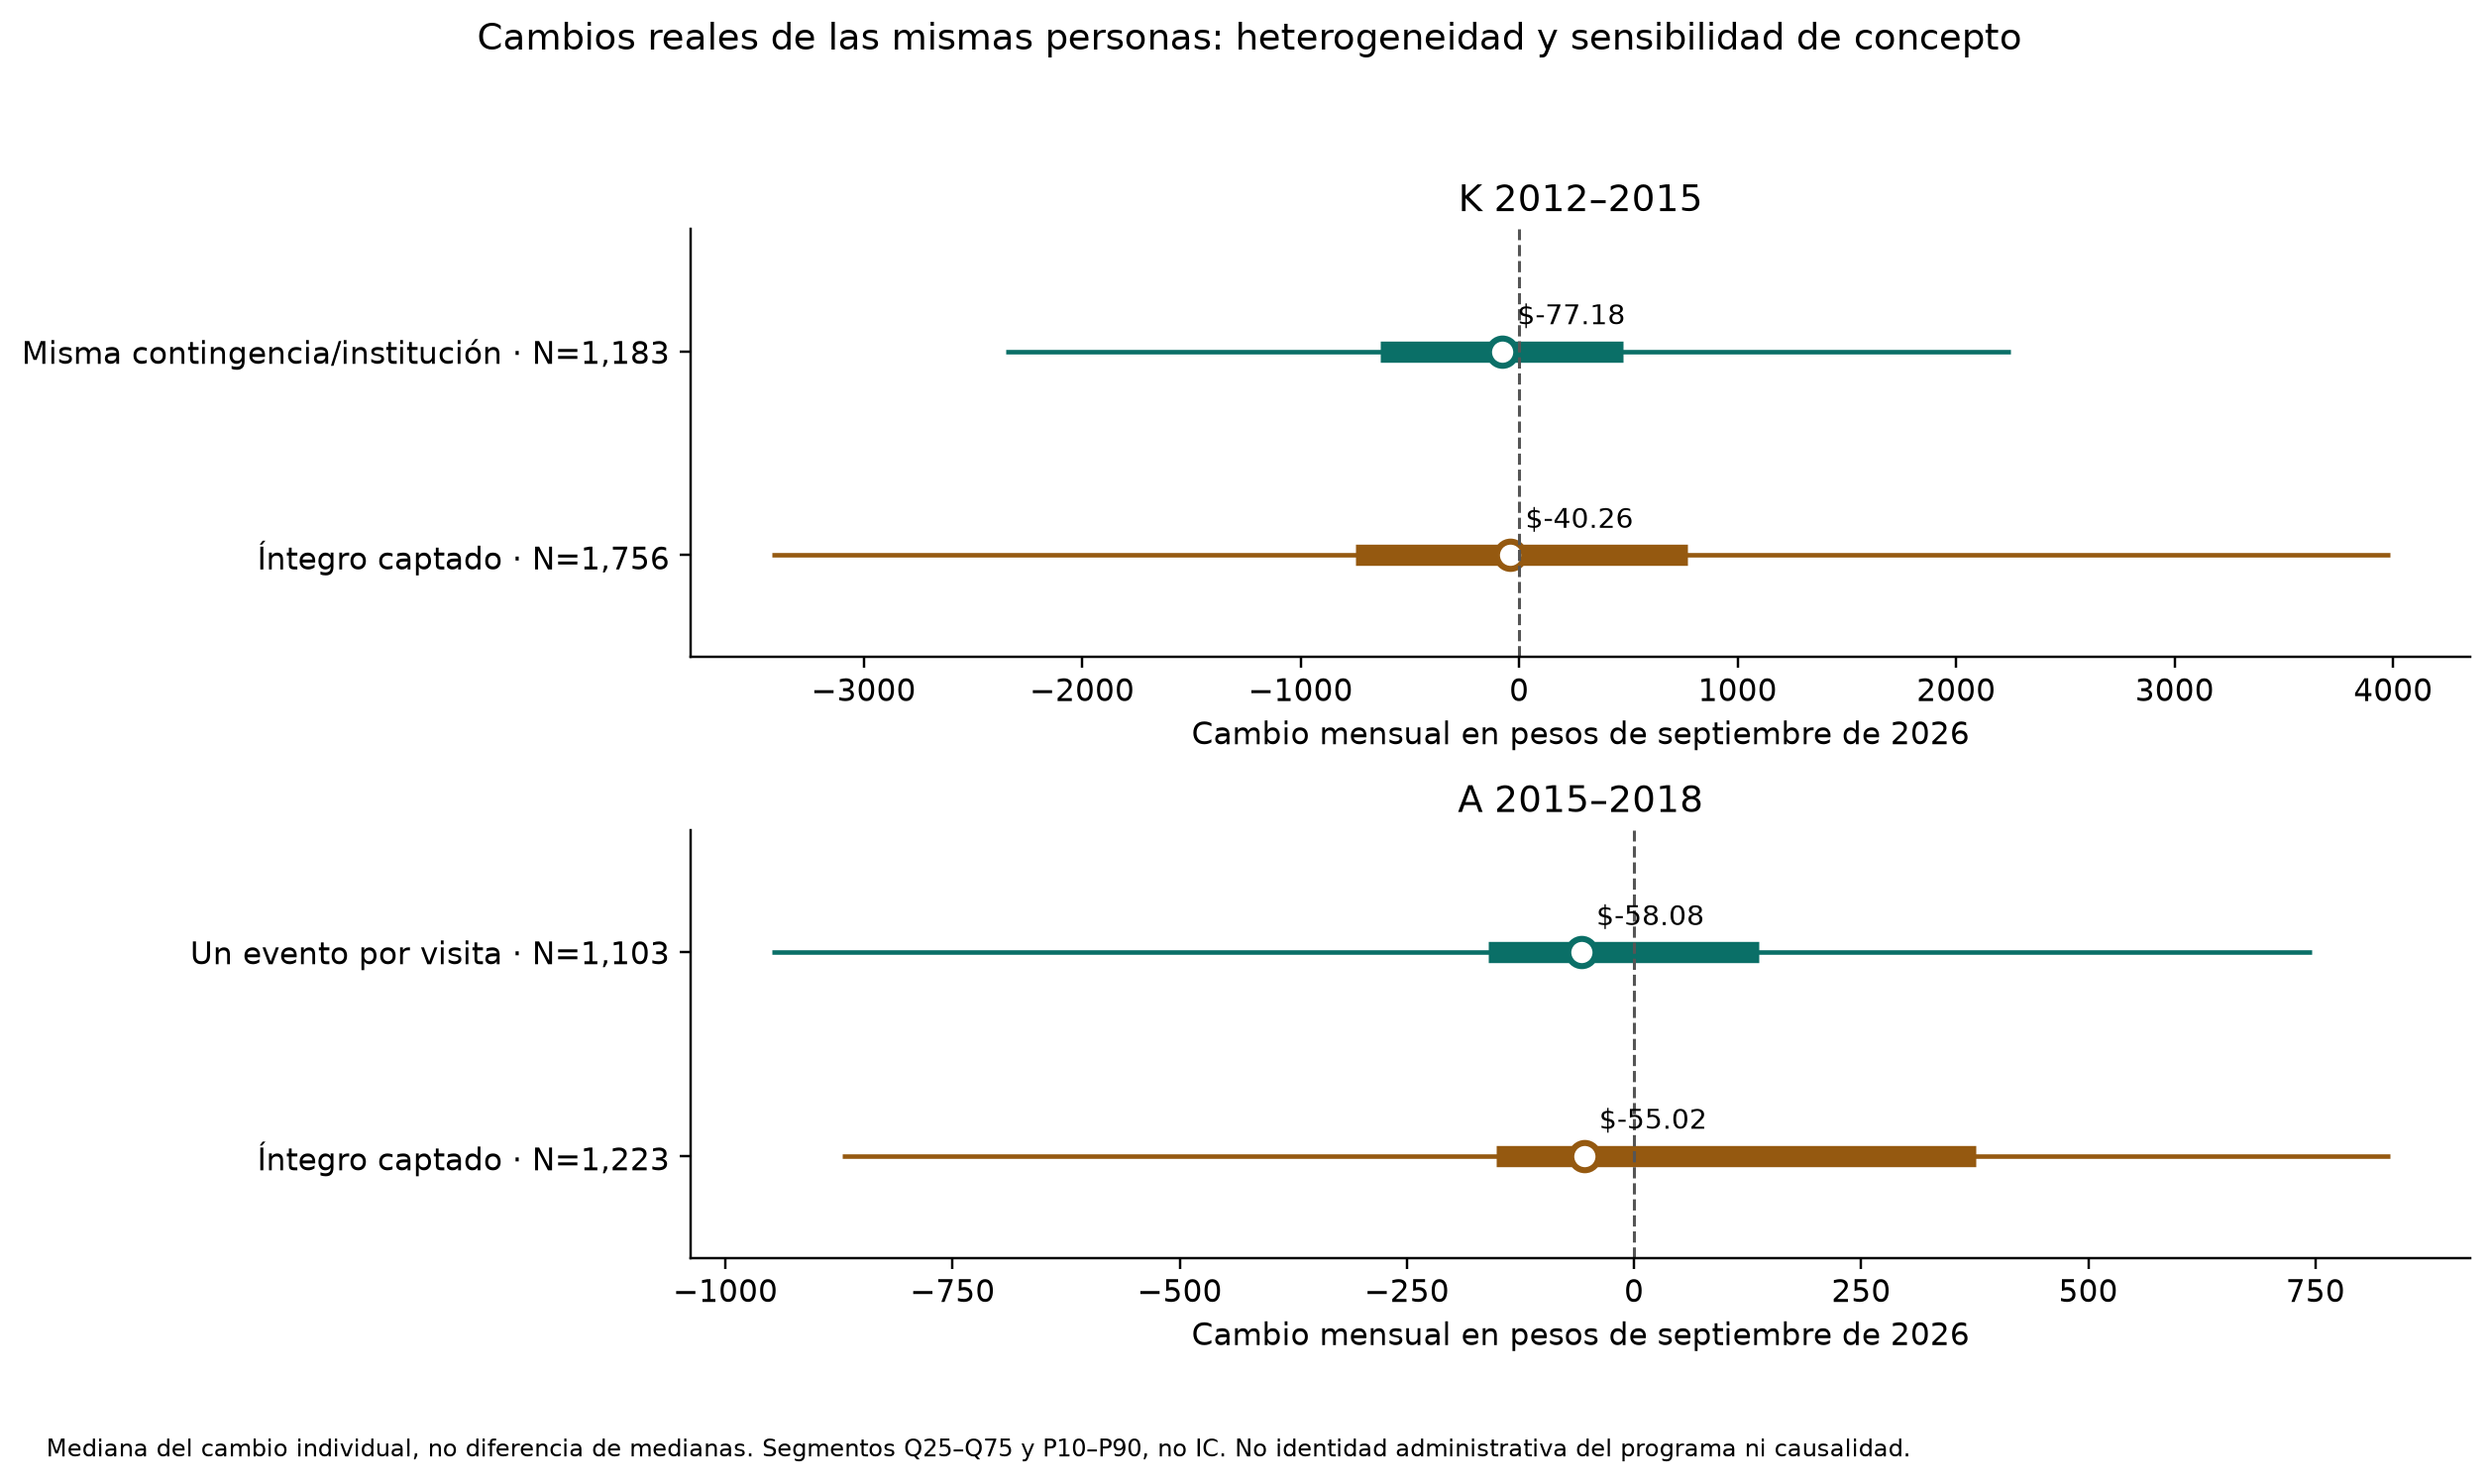
\includegraphics[width=\linewidth,height=.72\textheight,keepaspectratio]{../resultados/figuras/transiciones_montos__cambios_personales.png}
\notacuadro{K 2012--2015 y A 2015--2018; directas 60+ basales. Principal: N=1\,756/1\,223 pares íntegros. Sensibilidades: K con un evento y misma contingencia/institución, N=1\,183; A con un evento por visita, N=1\,103. Estas restricciones cambian la población y no acreditan identidad administrativa. Las barras son cuantiles del cambio, no IC; la precisión de los contrastes seleccionados aparece en el cuadro~\ref{tab:tesis-cambios}.}
\fuentecuadro{Elaboración propia, agregados longitudinales e Informe General, figura 47. Pesos mensuales de septiembre de 2026.}
\end{figure}
\end{landscape}
\FloatBarrier

Quedan \dato{K.SinCambio} continuos K y \dato{A.SinCambio} A sin cambio
calculable entre todos los Sí$\rightarrow$Sí conocidos. Las cotas externas
de mediana que admiten posiciones extremas de sus cambios faltantes son
\dato{K.CotaCambio} y \dato{A.CotaCambio}, respectivamente.
K puede cruzar cero; A conserva signo negativo bajo el criterio temporal
principal de ese ejercicio. Son cotas de información incompleta, no
intervalos conjuntos de muestreo y faltantes. No incluyen a personas
fallecidas o ausentes.

\section{Sensibilidad a mortalidad y pérdida de seguimiento}
\label{sec:resultados-seleccion}

De la cohorte basal K de \dato{K.Basal} personas, se registran
\dato{K.Muertes} fallecimientos, \dato{K.Ausencias} ausencias de estado
vital desconocido y \dato{K.Sustitutos} sustitutos vivos en destino.
Para A, entre \dato{A.Basal}, los conteos son
\dato{A.Muertes}, \dato{A.Ausencias} y \dato{A.Sustitutos}.
Un conflicto vital A se mantiene separado del principal.
No se suman estos destinos a las negativas de recepción.

Los agregados de seguimiento muestran diferencias según recepción basal,
pero la dirección de la ausencia no es uniforme entre vías.
La cohorte inicial y los pares monetarios observados responden, por ello,
a poblaciones diferentes. Las reapariciones posteriores confirman que
ausencia no equivale a muerte ni a pérdida definitiva.

Permitir sustitutos válidos en destino mantiene las medianas generales
de nuevos y continuos K/A con N mayores, sin acreditar ausencia de sesgo
en los subgrupos. Estandarizar composición de observados tampoco recupera
los importes de quienes no se observan. La mortalidad completa, la selección
no observada y los montos de toda la cohorte siguen sin identificarse.
No se ofrecen trayectorias imputadas después del fallecimiento ni una
corrección por probabilidad de observación.

\section{Síntesis de resultados frente a la hipótesis}
\label{sec:resultados-sintesis}

H1 encuentra respaldo localizado: en K 2012--2015 y A 2015--2018,
mayor recepción coincide con menor mediana real transversal.
El aumento real K 2018--2021 impide extender esa lectura a todo el periodo.
Además, la comparación transversal no describe la pérdida personal de
todos los receptores.

Para H2, el contraste K entre nuevos y continuos es grande en la definición
original y persiste bajo composición común, pero su magnitud se reduce
sustancialmente bajo la sensibilidad institucional; su lectura cambia al examinar evidencia
IMSS/ISSSTE. A presenta el nulo mediano relevante. Las ventanas y conceptos
son diferentes: no se ha estimado un efecto común ni una interacción
causal entre programas.

H3 es consistente con la reducción de brecha de unión y con brechas de
monto positivas en los dos cortes. No se establece con precisión el
ensanchamiento monetario. La figura~\ref{fig:tesis-precision} reúne la
precisión de los contrastes y muestra dónde los intervalos incluyen cero.

\begin{landscape}
\begin{figure}[p]
\centering
\caption{Precisión condicional de incorporación, continuidad y brechas por sexo}
\label{fig:tesis-precision}
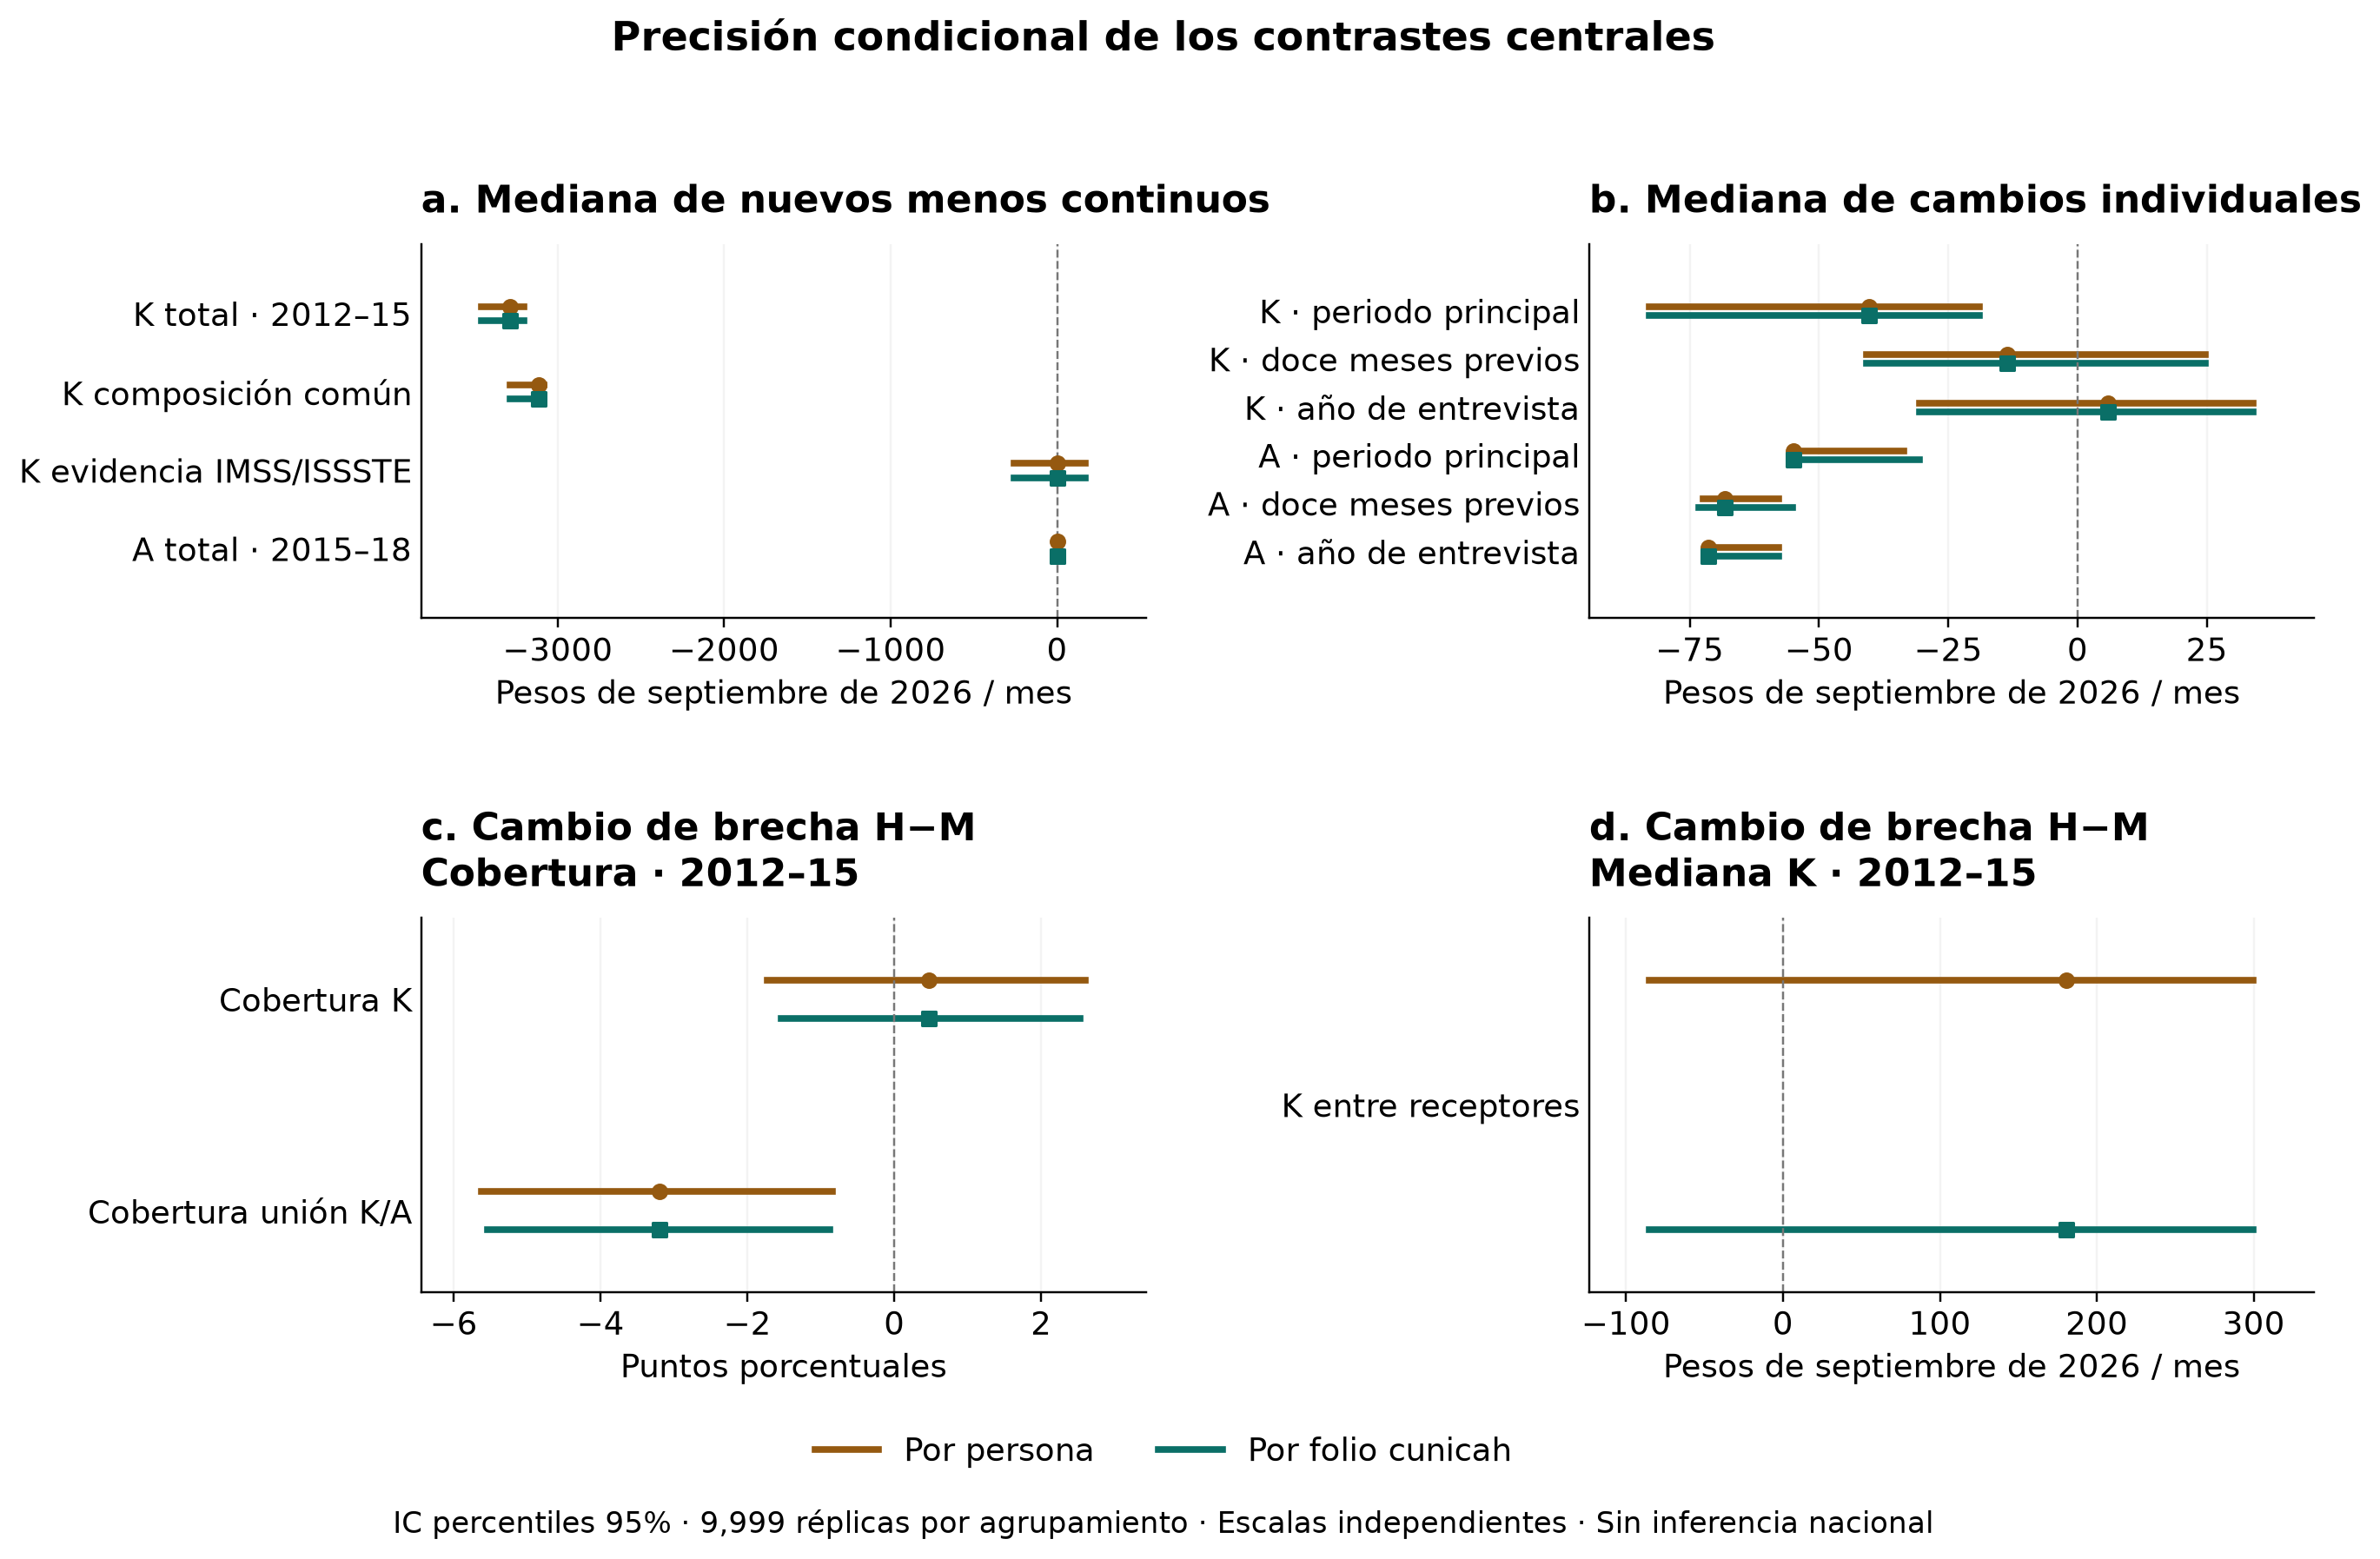
\includegraphics[width=\linewidth,height=.72\textheight,keepaspectratio]{../resultados/figuras/transiciones_montos__precision.png}
\notacuadro{IC percentiles 95\%, 9\,999 réplicas por persona y sensibilidad por folio. Paneles de incorporación: montos de destino; cambios individuales: pares K/A; brechas: cortes dinámicos2012/2015. Las escalas de pesos y puntos porcentuales difieren por panel. N en cuadros~\ref{tab:tesis-incorporacion}--\ref{tab:tesis-cambios} y~\ref{tab:tesis-sexo}. No hay inferencia de diseño nacional.}
\fuentecuadro{Validación focalizada reproducible de los agregados06--08; Informe General, figura 48 y sección 10.7. Pesos de septiembre de 2026.}
\end{figure}
\end{landscape}
\FloatBarrier

El balance respalda una relación no uniforme entre ampliación de acceso
y niveles de recursos captados, acotada a las definiciones y ventanas
verificadas; no identifica una mejora del ingreso total.
La precisión muestral refuerza algunos contrastes y limita otros;
no convierte la hipótesis general en una conclusión nacional demostrada
ni identifica mecanismos causales de política pública.



% BEGIN calidad10
\section{Calidad del soporte y robustez de las comparaciones}
\label{sec:resultados-calidad10}

K 2001--2003 no permite una conclusión monetaria direccional P/C: C tiene
11 montos válidos y dividirlo en cuartiles genera ramas de muy baja frecuencia.
Las mitades patrimoniales no rescatan ese soporte. Se conservan sus originales
privados y el no estimado; no se agrupan ventanas para obtener precisión.

\begingroup\small\setlength{\tabcolsep}{3pt}
\begin{longtable}{lrrrp{.21\textwidth}}
\caption{Precisión monetaria P menos C y estabilidad de remuestreo}\label{tab:calidad-tesis_calidad_precision}\\
\toprule
Vía/ventana & N P/C & IC semilla1 & IC semilla2 & Evaluación \\
\midrule\endfirsthead
\multicolumn{5}{l}{Continuación del cuadro \thetable}\\
\toprule
Vía/ventana & N P/C & IC semilla1 & IC semilla2 & Evaluación \\
\midrule\endhead
\bottomrule\endfoot
K 2001--2003 & 278/11 & No confiable & No confiable & Sin soporte direccional \\
K 2012--2015 & 1,060/373 & [51.4; 668.3] & [51.4; 409.1] & Dirección cruda estable \\
K 2018--2021 & 360/132 & [543.9; 1,324.3] & [543.9; 1,281.3] & Dirección cruda estable \\
A 2003--2012 & 666/98 & [0.0; 0.0] & [0.0; 0.0] & Condicional; empates \\
A 2012--2015 & 1,196/286 & [0.0; 0.0] & [0.0; 0.0] & Condicional; empates \\
A 2015--2018 & 581/589 & [-30.6; 7.6] & [-30.6; 7.6] & Medianas coincidentes \\
\end{longtable}
{\footnotesize Fuente: auditoría10, insumos01--09 intactos. Muestra sin ponderación; IC condicionales, sin inferencia nacional o causal. P: primera vía observada; C: otra vía basal afirmativa. 9999 réplicas por folio y dos semillas. Se muestran estimación e IC. Los intervalos por orden e influencia están en el informe. La diferencia K2001--2003 no se usa como conclusión direccional aunque pueda calcularse.\par}
\endgroup

\begingroup\small\setlength{\tabcolsep}{3pt}
\begin{longtable}{lrrr}
\caption{Sensibilidad del gradiente patrimonial de incorporación}\label{tab:calidad-tesis_calidad_gradiente}\\
\toprule
Vía/ventana & Edad3/celda20 pp & Edad2/celda30 pp & N soporte Q1/Q4 \\
\midrule\endfirsthead
\multicolumn{4}{l}{Continuación del cuadro \thetable}\\
\toprule
Vía/ventana & Edad3/celda20 pp & Edad2/celda30 pp & N soporte Q1/Q4 \\
\midrule\endhead
\bottomrule\endfoot
K 2001--2003 & -0.5 [-3.1; 1.9] & -0.8 [-3.2; 1.7] & 956/831 \\
K 2012--2015 & 0.5 [-4.0; 5.0] & 0.3 [-4.2; 4.9] & 918/894 \\
K 2018--2021 & -4.0 [-7.7; -0.4] & -4.0 [-7.6; -0.4] & 668/596 \\
A 2003--2012 & 6.8 [0.3; 13.2] & 6.9 [0.9; 13.3] & 527/499 \\
A 2012--2015 & 4.0 [-0.8; 8.6] & 4.0 [-1.0; 8.8] & 919/895 \\
A 2015--2018 & 6.2 [0.7; 11.6] & 4.7 [-0.8; 10.2] & 508/490 \\
\end{longtable}
{\footnotesize Fuente: auditoría10, insumos01--09 intactos. Muestra sin ponderación; IC condicionales, sin inferencia nacional o causal. P: primera vía observada; C: otra vía basal afirmativa. Q1 menos Q4 entre negativas K/A reobservadas; sexo y escolaridad se mantienen. Edad2=60--69/70+, edad3=60--64/65--69/70+. Cambian soporte y mezcla, no es la misma población. Todas las cuatro especificaciones están en el informe; no se elige por significancia.\par}
\endgroup


Los cuadros registran todas las variantes, sin escoger las que excluyen cero.
A 2003--2012 mantiene gradiente positivo en las especificaciones viables,
pero A 2015--2018 y K 2018--2021 dependen del soporte; A 2012--2015 incluye
cero tras ajuste. Los P--C K recientes conservan dirección cruda con dos
semillas, pero el extremo superior K 2012--2015 es inestable. La robustez
al remuestreo no implica robustez a la medición institucional. Los empates A
se conservan sin inferir equivalencia.

\begingroup\small\setlength{\tabcolsep}{3pt}
\begin{longtable}{lp{.26\textwidth}rrp{.15\textwidth}}
\caption{Soporte de los contrastes institucionales P menos C}\label{tab:calidad-tesis_calidad_instituciones}\\
\toprule
Vía/ventana & Institución & N P/C & Diferencia [IC95] & Uso \\
\midrule\endfirsthead
\multicolumn{5}{l}{Continuación del cuadro \thetable}\\
\toprule
Vía/ventana & Institución & N P/C & Diferencia [IC95] & Uso \\
\midrule\endhead
\bottomrule\endfoot
K 2001--2003 & Evidencia IMSS/ISSSTE & 244/$<$10 & No estimable & No confiable \\
K 2001--2003 & Programas agrupados & 0/0 & No estimable & No confiable \\
K 2001--2003 & Un evento IMSS & 214/$<$10 & No estimable & No confiable \\
K 2001--2003 & Un evento ISSSTE & 25/$<$10 & No estimable & No confiable \\
K 2012--2015 & Evidencia IMSS/ISSSTE & 406/27 & 513.5 [0.0; 1,027.1] & Exploratorio 10--29 \\
K 2012--2015 & Programas agrupados & 599/326 & 0.0 [0.0; 0.0] & Sin equivalencia \\
K 2012--2015 & Un evento IMSS & 305/20 & 428.0 [0.0; 684.7] & Exploratorio 10--29 \\
K 2012--2015 & Un evento ISSSTE & 63/$<$10 & No estimable & No confiable \\
K 2018--2021 & Evidencia IMSS/ISSSTE & 309/79 & 679.9 [-61.2; 1,087.8] & Exploratorio \\
K 2018--2021 & Programas agrupados & 0/0 & No estimable & No confiable \\
K 2018--2021 & Un evento IMSS & 259/68 & 271.9 [-192.4; 679.9] & Exploratorio \\
K 2018--2021 & Un evento ISSSTE & 33/10 & No estimable & No confiable \\
\end{longtable}
{\footnotesize Fuente: auditoría10, insumos01--09 intactos. Muestra sin ponderación; IC condicionales, sin inferencia nacional o causal. P: primera vía observada; C: otra vía basal afirmativa. Conteos monetarios pequeños se indican como menos de10. Las ramas con10--29 se revisaron por amplitud e influencia: las viables se conservan como exploratorias, incluyan o no cero. Las no confiables se indican sin estimación. No se mezclan instituciones para obtener N. Sin programa común longitudinalA.\par}
\endgroup


Institución y evento único reducen el soporte; las ramas de 20--29 válidos
C son exploratorias y las insuficientes no se usan para concluir dirección.
La comparación siguiente es contexto transversal por escolaridad agrupada,
no una respuesta causal ni longitudinal. Su universo de 60+ incluye modalidades
distintas de la muestra directa principal; ND se conserva como información
insuficiente, no como perfil económico.
\begingroup\small\setlength{\tabcolsep}{3pt}
\begin{longtable}{lrrrrr}
\caption{Reformulación del contexto patrimonial por escolaridad y titularidad,2021}\label{tab:calidad-tesis_calidad_T8}\\
\toprule
Titularidad K & Esc. años & N & Q25 & Mediana & Q75 \\
\midrule\endfirsthead
\multicolumn{6}{l}{Continuación del cuadro \thetable}\\
\toprule
Titularidad K & Esc. años & N & Q25 & Mediana & Q75 \\
\midrule\endhead
\bottomrule\endfoot
Ambas & 0--5 & 84 & 419.9 & 805.6 & 1,088.3 \\
Ambas & 6+ & 384 & 800.0 & 1,580.0 & 2,769.7 \\
Ambas negativas K & 0--5 & 3,251 & 90.0 & 450.0 & 1,000.0 \\
Ambas negativas K & 6+ & 2,377 & 152.0 & 650.0 & 1,382.7 \\
Solo cónyuge & 0--5 & 385 & 400.0 & 800.0 & 1,505.0 \\
Solo cónyuge & 6+ & 677 & 530.0 & 1,050.0 & 2,022.0 \\
Solo propia & 0--5 & 996 & 224.9 & 650.8 & 1,222.5 \\
Solo propia & 6+ & 2,067 & 400.0 & 914.3 & 1,800.7 \\
\end{longtable}
{\footnotesize Fuente: EDA original60+ por visita, incluidas modalidades originales; no es la población principal directa09. Patrimonio compartido, miles de unidades almacenadas, no pesos reales. Escolaridad0--5/6+; titularidad o escolaridad ND quedan como exclusiones. Se presentan todos los grupos, no máximos seleccionados.\par}
\endgroup

% END calidad10

\chapter{Discusión y conclusiones}
\label{cap:discusion}
\estadoBorrador

La discusión final permanece abierta; esta etapa identifica preguntas
sustentadas por resultados exploratorios. La propuesta predictiva anterior
se conserva únicamente como antecedente posible. Una eventual discusión de
esa línea se redactaría a partir de resultados evaluados y aprobados.
En esa posible línea futura se contrastarían las hipótesis y se identificarían
limitaciones de selección y
medición, delimitar la aplicabilidad de las alertas y separar asociación
predictiva de inferencia causal. La auditoría actual sustenta la necesidad
de distinguir modalidades, fechas y poblaciones; no demuestra todavía una
ganancia predictiva ni una anticipación útil para intervenir.

% BEGIN CONSOLIDATED 05_preguntas_exploratorias
\section{Posibles líneas de investigación derivadas de los hallazgos}

\label{sec:exploracion-preguntas}

Las siguientes líneas se derivan de los agregados observados y permanecen abiertas. Su prioridad depende de interés sustantivo, cobertura y validación, no de seleccionar un outcome predeterminado. No se estima un modelo ni se aprueba una pregunta definitiva.

\subsection{¿Cómo difiere la recepción propia y del cónyuge por sexo y escolaridad inicial?}

Resultado que motiva: T1\_2021: brecha propia de 18,59 pp en 6 años y 0,55 pp en $\geq$10 años.

Variables y rondas: K propia/cónyuge, sexo, escolaridad inicial, edad, estado conyugal. Perfiles transversales seis rondas; trayectorias condicionadas K2001--2003/2012--2015/2018--2021.

Viabilidad: Validar J1/2001, filtros de pareja, selección y antecedente laboral. Descriptiva estratificada; econométrica asociacional tras fijar estimando; predicción solo futura y opcional.

\subsection{¿En qué perfiles coexisten pensiones K y apoyos, y cómo varía la coexistencia con la edad?}

Resultado que motiva: 2021: 2\,019 K+A; 3\,558 A con negativa K; V=0,03756 y tasas de A muy diferentes por edad quinquenal.

Variables y rondas: K/A propios, edad, sexo, escolaridad, localidad; programa explícito cuando existe. Cortes seis rondas con contratos separados; recepción conjunta 2012--2015 condicionada; A2018--2021 no homologado.

Viabilidad: No llamar sin pensión a negativa K ni todo A no contributivo; separar dinero/especie requeriría fuente adicional. Descriptiva/econométrica sin causalidad por defecto.

\subsection{¿Qué continuidad e inicio de apoyo se observa entre personas con negativa K inicial?}

Resultado que motiva: Cohorte con negativa K en 2015, 60+ viva: 5\,503 personas. Inicio A observado 653/2\,740 con negativa A inicial y respuesta final conocida (23,83\%). Mismo donativo adicional, dinero/especie; 2018 desglosa hasta dos instituciones. Solo recepción agregada condicionada.. No equivale a personas sin toda pensión, ni implica que el apoyo haya causado ampliación de cobertura.

Variables y rondas: K en origen, A en ambos momentos, perfiles iniciales, seguimiento y modalidades. A2003--2012/2012--2015/2015--2018 condicionados; intervalos nominales desiguales.

Viabilidad: Necesita examinar selección de pares conocidos, retornos, muerte y sensibilidad. Descriptiva panel; modelo de transición asociacional si se define proceso de observación y estimando.

\subsection{¿Cómo se combinan recepción pensionaria y trabajo durante el envejecimiento?}

Resultado que motiva: 2021: 559/2\,760 (20,25\%) K propia entre quienes trabajan; T7 presenta heterogeneidad por edad.

Variables y rondas: Ocupación construida, edad, K propia/cónyuge, salario principal en elegibles, instituciones. Actividad en seis ondas; recepción K longitudinal solo en periodos compatibles.

Viabilidad: Ocupación no profesión; retiro/incapacidad/no trabajo no separables. Validar saltos y periodos salarial/pensionario. Descripción de perfiles y transiciones; econometría asociacional, no efecto retiro.

\subsection{¿Qué diferencias institucionales aparecen entre receptoras según escolaridad y localidad?}

Resultado que motiva: 2021: IMSS 2\,540/3\,592; instituciones múltiples no aditivas. C1/C2 usan perfiles simultáneos.

Variables y rondas: Instituciones fuente, contingencia, sexo, edad, educación, localidad, titularidad. Seis cortes por instrumento; cambios institucionales individuales requieren homologación adicional, especialmente2012/2015.

Viabilidad: Fuente no régimen y código ambiguo permanece desconocido. No asignar monto por institución cuando selección por contingencia. Descriptiva; transición institucional pendiente, no entrenar un modelo.

\subsection{¿Cómo varía la asociación de monto pensionario propio y patrimonio compartido por escolaridad?}

Resultado que motiva: 2021: Spearman 0,2643 en 3\,347 pares; T8 distribuye patrimonio simultáneamente por ramas y educación.

Variables y rondas: Patrimonio, monto K parcial, escolaridad, tipo/slot, titular y pareja. Distribuciones internas a seis rondas; cambio real no disponible hasta validar moneda/precios y unidad compartida.

Viabilidad: No vulnerabilidad por cuartil, no ingreso total y no acumulación causal. Descriptiva actual; longitudinal monetaria pendiente de deflactor y consistencia de unidad.
% END CONSOLIDATED 05_preguntas_exploratorias


\bibliographystyle{plainnat}
\bibliography{../investigacion/referencias}
\appendix
\chapter{Tablas complementarias de CP1}
\label{ap:tablas-cp1}

Las distribuciones siguientes conservan toda la población de cada ronda y
explicitan sus faltantes. Son complementos de la descripción del
capítulo~\ref{cap:datos}; sus cambios no se atribuyen automáticamente a
transiciones dentro de persona. La documentación exhaustiva de las 119
variables, doce alternativas y matrices de modalidades permanece en Jupyter
y en los informes de CP1.

% Generado: no editar cifras manualmente.
\begin{table}[!htbp]
\centering
\caption{Sexo registrado por ronda}\label{tab:cp1-sexo}
\small\setlength{\tabcolsep}{4pt}
\renewcommand{\arraystretch}{1.15}
\begin{tabular}{p{0.28\linewidth}rrrrrr}
\toprule
\textbf{Categoría} & \textbf{2001} & \textbf{2003} & \textbf{2012} & \textbf{2015} & \textbf{2018} & \textbf{2021} \\
\midrule
Hombre & \shortstack[r]{6\,503\\(42,82\%)} & \shortstack[r]{6\,108\\(42,86\%)} & \shortstack[r]{8\,000\\(43,33\%)} & \shortstack[r]{6\,739\\(42,15\%)} & \shortstack[r]{7\,761\\(42,53\%)} & \shortstack[r]{7\,446\\(42,46\%)} \\
Mujer & \shortstack[r]{8\,683\\(57,18\%)} & \shortstack[r]{8\,142\\(57,14\%)} & \shortstack[r]{10\,465\\(56,67\%)} & \shortstack[r]{9\,249\\(57,85\%)} & \shortstack[r]{10\,488\\(57,47\%)} & \shortstack[r]{10\,092\\(57,54\%)} \\
\bottomrule
\end{tabular}
\par\medskip
\parbox{\linewidth}{\footnotesize Fuente: elaboración propia con agregados de CP1, ENASEMsimple v2 (2001--2021). Frecuencias sin ponderación. Cada celda: n y (\%). Denominador: todos los registros de la ronda de la tabla de población, incluidos faltantes. Las categorías suman N; un código ausente tiene frecuencia cero.}
\end{table}

% Generado: no editar cifras manualmente.
\begin{table}[!htbp]
\centering
\caption{Escolaridad agrupada por ronda}\label{tab:cp1-edu-gru}
\small\setlength{\tabcolsep}{4pt}
\renewcommand{\arraystretch}{1.15}
\begin{tabular}{p{0.28\linewidth}rrrrrr}
\toprule
\textbf{Categoría} & \textbf{2001} & \textbf{2003} & \textbf{2012} & \textbf{2015} & \textbf{2018} & \textbf{2021} \\
\midrule
Sin escolaridad & \shortstack[r]{3\,652\\(24,05\%)} & \shortstack[r]{3\,517\\(24,68\%)} & \shortstack[r]{3\,699\\(20,03\%)} & \shortstack[r]{2\,847\\(17,81\%)} & \shortstack[r]{2\,657\\(14,56\%)} & \shortstack[r]{2\,418\\(13,79\%)} \\
1--5 años & \shortstack[r]{5\,239\\(34,50\%)} & \shortstack[r]{4\,945\\(34,70\%)} & \shortstack[r]{5\,728\\(31,02\%)} & \shortstack[r]{4\,757\\(29,75\%)} & \shortstack[r]{4\,620\\(25,32\%)} & \shortstack[r]{4\,321\\(24,64\%)} \\
6 años & \shortstack[r]{2\,788\\(18,36\%)} & \shortstack[r]{2\,611\\(18,32\%)} & \shortstack[r]{3\,694\\(20,01\%)} & \shortstack[r]{3\,310\\(20,70\%)} & \shortstack[r]{3\,801\\(20,83\%)} & \shortstack[r]{3\,645\\(20,78\%)} \\
7--9 años & \shortstack[r]{1\,988\\(13,09\%)} & \shortstack[r]{1\,774\\(12,45\%)} & \shortstack[r]{2\,938\\(15,91\%)} & \shortstack[r]{2\,732\\(17,09\%)} & \shortstack[r]{3\,676\\(20,14\%)} & \shortstack[r]{3\,583\\(20,43\%)} \\
10 años o más & \shortstack[r]{1\,500\\(9,88\%)} & \shortstack[r]{1\,304\\(9,15\%)} & \shortstack[r]{2\,312\\(12,52\%)} & \shortstack[r]{2\,162\\(13,52\%)} & \shortstack[r]{3\,335\\(18,27\%)} & \shortstack[r]{3\,247\\(18,51\%)} \\
.d & \shortstack[r]{18\\(0,12\%)} & \shortstack[r]{22\\(0,15\%)} & \shortstack[r]{14\\(0,08\%)} & \shortstack[r]{122\\(0,76\%)} & \shortstack[r]{96\\(0,53\%)} & \shortstack[r]{97\\(0,55\%)} \\
.r & \shortstack[r]{1\\(0,01\%)} & \shortstack[r]{1\\(0,01\%)} & \shortstack[r]{0\\(0,00\%)} & \shortstack[r]{0\\(0,00\%)} & \shortstack[r]{7\\(0,04\%)} & \shortstack[r]{6\\(0,03\%)} \\
.m & \shortstack[r]{0\\(0,00\%)} & \shortstack[r]{67\\(0,47\%)} & \shortstack[r]{50\\(0,27\%)} & \shortstack[r]{51\\(0,32\%)} & \shortstack[r]{51\\(0,28\%)} & \shortstack[r]{205\\(1,17\%)} \\
.f & \shortstack[r]{0\\(0,00\%)} & \shortstack[r]{9\\(0,06\%)} & \shortstack[r]{30\\(0,16\%)} & \shortstack[r]{7\\(0,04\%)} & \shortstack[r]{6\\(0,03\%)} & \shortstack[r]{16\\(0,09\%)} \\
\bottomrule
\end{tabular}
\par\medskip
\parbox{\linewidth}{\footnotesize Fuente: elaboración propia con agregados de CP1, ENASEMsimple v2 (2001--2021). Frecuencias sin ponderación. Cada celda: n y (\%). Denominador: todos los registros de la ronda de la tabla de población, incluidos faltantes. Las categorías suman N; un código ausente tiene frecuencia cero.}
\end{table}

% Generado: no editar cifras manualmente.
\begin{table}[!htbp]
\centering
\caption{Estado conyugal por ronda}\label{tab:cp1-est-conyugal}
\small\setlength{\tabcolsep}{4pt}
\renewcommand{\arraystretch}{1.15}
\begin{tabular}{p{0.28\linewidth}rrrrrr}
\toprule
\textbf{Categoría} & \textbf{2001} & \textbf{2003} & \textbf{2012} & \textbf{2015} & \textbf{2018} & \textbf{2021} \\
\midrule
Casado o en unión & \shortstack[r]{10\,512\\(69,22\%)} & \shortstack[r]{9\,689\\(67,99\%)} & \shortstack[r]{10\,910\\(59,08\%)} & \shortstack[r]{9\,862\\(61,68\%)} & \shortstack[r]{11\,838\\(64,87\%)} & \shortstack[r]{10\,295\\(58,70\%)} \\
Separado o divorciado & \shortstack[r]{1\,144\\(7,53\%)} & \shortstack[r]{947\\(6,65\%)} & \shortstack[r]{1\,231\\(6,67\%)} & \shortstack[r]{1\,473\\(9,21\%)} & \shortstack[r]{1\,325\\(7,26\%)} & \shortstack[r]{1\,278\\(7,29\%)} \\
Viudo & \shortstack[r]{2\,535\\(16,69\%)} & \shortstack[r]{2\,545\\(17,86\%)} & \shortstack[r]{2\,860\\(15,49\%)} & \shortstack[r]{2\,829\\(17,69\%)} & \shortstack[r]{3\,047\\(16,70\%)} & \shortstack[r]{3\,448\\(19,66\%)} \\
Soltero & \shortstack[r]{539\\(3,55\%)} & \shortstack[r]{522\\(3,66\%)} & \shortstack[r]{722\\(3,91\%)} & \shortstack[r]{615\\(3,85\%)} & \shortstack[r]{904\\(4,95\%)} & \shortstack[r]{718\\(4,09\%)} \\
.m & \shortstack[r]{456\\(3,00\%)} & \shortstack[r]{0\\(0,00\%)} & \shortstack[r]{0\\(0,00\%)} & \shortstack[r]{0\\(0,00\%)} & \shortstack[r]{0\\(0,00\%)} & \shortstack[r]{0\\(0,00\%)} \\
.f & \shortstack[r]{0\\(0,00\%)} & \shortstack[r]{546\\(3,83\%)} & \shortstack[r]{2\,742\\(14,85\%)} & \shortstack[r]{1\,209\\(7,56\%)} & \shortstack[r]{1\,135\\(6,22\%)} & \shortstack[r]{1\,799\\(10,26\%)} \\
.d & \shortstack[r]{0\\(0,00\%)} & \shortstack[r]{1\\(0,01\%)} & \shortstack[r]{0\\(0,00\%)} & \shortstack[r]{0\\(0,00\%)} & \shortstack[r]{0\\(0,00\%)} & \shortstack[r]{0\\(0,00\%)} \\
\bottomrule
\end{tabular}
\par\medskip
\parbox{\linewidth}{\footnotesize Fuente: elaboración propia con agregados de CP1, ENASEMsimple v2 (2001--2021). Frecuencias sin ponderación. Cada celda: n y (\%). Denominador: todos los registros de la ronda de la tabla de población, incluidos faltantes. Las categorías suman N; un código ausente tiene frecuencia cero.}
\end{table}

% Generado: no editar cifras manualmente.
\begin{table}[!htbp]
\centering
\caption{Tamaño de localidad por ronda}\label{tab:cp1-urbano}
\small\setlength{\tabcolsep}{4pt}
\renewcommand{\arraystretch}{1.15}
\begin{tabular}{p{0.28\linewidth}rrrrrr}
\toprule
\textbf{Categoría} & \textbf{2001} & \textbf{2003} & \textbf{2012} & \textbf{2015} & \textbf{2018} & \textbf{2021} \\
\midrule
Menos de 100 mil residentes & \shortstack[r]{6\,229\\(41,02\%)} & \shortstack[r]{5\,777\\(40,54\%)} & \shortstack[r]{6\,600\\(35,74\%)} & \shortstack[r]{6\,329\\(39,59\%)} & \shortstack[r]{7\,590\\(41,59\%)} & \shortstack[r]{6\,936\\(39,55\%)} \\
100 mil residentes o más & \shortstack[r]{8\,957\\(58,98\%)} & \shortstack[r]{7\,927\\(55,63\%)} & \shortstack[r]{9\,123\\(49,41\%)} & \shortstack[r]{8\,450\\(52,85\%)} & \shortstack[r]{9\,524\\(52,19\%)} & \shortstack[r]{8\,803\\(50,19\%)} \\
.f & \shortstack[r]{0\\(0,00\%)} & \shortstack[r]{546\\(3,83\%)} & \shortstack[r]{2\,742\\(14,85\%)} & \shortstack[r]{1\,209\\(7,56\%)} & \shortstack[r]{1\,135\\(6,22\%)} & \shortstack[r]{1\,799\\(10,26\%)} \\
\bottomrule
\end{tabular}
\par\medskip
\parbox{\linewidth}{\footnotesize Fuente: elaboración propia con agregados de CP1, ENASEMsimple v2 (2001--2021). Frecuencias sin ponderación. Cada celda: n y (\%). Denominador: todos los registros de la ronda de la tabla de población, incluidos faltantes. Las categorías suman N; un código ausente tiene frecuencia cero.}
\end{table}

\clearpage
% Generado: no editar cifras manualmente.
\begingroup\small
\setlength{\tabcolsep}{4pt}
\begin{longtable}{rp{0.26\linewidth}rrrr}
\caption{Conservados y excluidos por alternativa y ronda}\label{tab:cp1-muestras-ronda}\\
\toprule
\textbf{Año} & \textbf{Alternativa} & \textbf{N original} & \textbf{Conservados} & \textbf{Excluidos} & \textbf{\% conservado} \\
\midrule\endfirsthead
\multicolumn{6}{l}{\textit{Continuación}}\\
\toprule
\textbf{Año} & \textbf{Alternativa} & \textbf{N original} & \textbf{Conservados} & \textbf{Excluidos} & \textbf{\% conservado} \\
\midrule\endhead
\bottomrule\endfoot
2001 & Universo completo & 15\,186 & 15\,186 & 0 & 100,00 \\
2001 & No balanceado & 15\,186 & 15\,186 & 0 & 100,00 \\
2001 & 60+ por visita & 15\,186 & 7\,416 & 7\,770 & 48,83 \\
2001 & Directas & 15\,186 & 14\,154 & 1\,032 & 93,20 \\
2001 & Directas 60+ & 15\,186 & 6\,812 & 8\,374 & 44,86 \\
2001 & Seis presencias & 15\,186 & 6\,305 & 8\,881 & 41,52 \\
2001 & Seis directas & 15\,186 & 3\,893 & 11\,293 & 25,64 \\
2001 & Seis directas 60+ & 15\,186 & 964 & 14\,222 & 6,35 \\
2003 & Universo completo & 14\,250 & 14\,250 & 0 & 100,00 \\
2003 & No balanceado & 14\,250 & 14\,250 & 0 & 100,00 \\
2003 & 60+ por visita & 14\,250 & 7\,691 & 6\,559 & 53,97 \\
2003 & Directas & 14\,250 & 12\,526 & 1\,724 & 87,90 \\
2003 & Directas 60+ & 14\,250 & 6\,970 & 7\,280 & 48,91 \\
2003 & Seis presencias & 14\,250 & 6\,305 & 7\,945 & 44,25 \\
2003 & Seis directas & 14\,250 & 3\,893 & 10\,357 & 27,32 \\
2003 & Seis directas 60+ & 14\,250 & 964 & 13\,286 & 6,76 \\
2012 & Universo completo & 18\,465 & 18\,465 & 0 & 100,00 \\
2012 & No balanceado & 18\,465 & 18\,465 & 0 & 100,00 \\
2012 & 60+ por visita & 18\,465 & 9\,886 & 8\,579 & 53,54 \\
2012 & Directas & 18\,465 & 14\,448 & 4\,017 & 78,25 \\
2012 & Directas 60+ & 18\,465 & 8\,888 & 9\,577 & 48,13 \\
2012 & Seis presencias & 18\,465 & 6\,305 & 12\,160 & 34,15 \\
2012 & Seis directas & 18\,465 & 3\,893 & 14\,572 & 21,08 \\
2012 & Seis directas 60+ & 18\,465 & 964 & 17\,501 & 5,22 \\
2015 & Universo completo & 15\,988 & 15\,988 & 0 & 100,00 \\
2015 & No balanceado & 15\,988 & 15\,988 & 0 & 100,00 \\
2015 & 60+ por visita & 15\,988 & 10\,416 & 5\,572 & 65,15 \\
2015 & Directas & 15\,988 & 13\,850 & 2\,138 & 86,63 \\
2015 & Directas 60+ & 15\,988 & 9\,640 & 6\,348 & 60,30 \\
2015 & Seis presencias & 15\,988 & 6\,305 & 9\,683 & 39,44 \\
2015 & Seis directas & 15\,988 & 3\,893 & 12\,095 & 24,35 \\
2015 & Seis directas 60+ & 15\,988 & 964 & 15\,024 & 6,03 \\
2018 & Universo completo & 18\,249 & 18\,249 & 0 & 100,00 \\
2018 & No balanceado & 18\,249 & 18\,249 & 0 & 100,00 \\
2018 & 60+ por visita & 18\,249 & 10\,113 & 8\,136 & 55,42 \\
2018 & Directas & 18\,249 & 15\,786 & 2\,463 & 86,50 \\
2018 & Directas 60+ & 18\,249 & 9\,107 & 9\,142 & 49,90 \\
2018 & Seis presencias & 18\,249 & 6\,305 & 11\,944 & 34,55 \\
2018 & Seis directas & 18\,249 & 3\,893 & 14\,356 & 21,33 \\
2018 & Seis directas 60+ & 18\,249 & 964 & 17\,285 & 5,28 \\
2021 & Universo completo & 17\,538 & 17\,538 & 0 & 100,00 \\
2021 & No balanceado & 17\,538 & 17\,538 & 0 & 100,00 \\
2021 & 60+ por visita & 17\,538 & 10\,482 & 7\,056 & 59,77 \\
2021 & Directas & 17\,538 & 14\,484 & 3\,054 & 82,59 \\
2021 & Directas 60+ & 17\,538 & 9\,424 & 8\,114 & 53,73 \\
2021 & Seis presencias & 17\,538 & 6\,305 & 11\,233 & 35,95 \\
2021 & Seis directas & 17\,538 & 3\,893 & 13\,645 & 22,20 \\
2021 & Seis directas 60+ & 17\,538 & 964 & 16\,574 & 5,50 \\
\end{longtable}
\noindent{\footnotesize Fuente: elaboración propia con agregados de CP1, ENASEMsimple v2 (2001--2021). Frecuencias sin ponderación. Cada conteo por ronda es tanto de registros como de personas, por unicidad persona-ronda. Conservados + excluidos = N original. Porcentaje sobre N original. No sumar personas entre rondas; las doce alternativas y composición están en el notebook.}
\endgroup


\chapter{Estado de redacción y pendientes de revisión}
\label{ap:pendientes}

La etapa vigente es exploratoria y pensionaria: no se ha aprobado pregunta
definitiva, hipótesis principal, outcome, definición de vulnerabilidad ni modelo.
Los pendientes predictivos anteriores se conservan como posibilidades futuras,
no como obligaciones de esta etapa. La matriz de cumplimiento v1 distingue
trabajo provisional, parcial y comparaciones no viables. Primero se requiere
profundizar contratos semánticos de las columnas candidatas, número declarado
de pensiones, montos salariales mes/año, titularidad e instrumentos.

Los capítulos~\ref{cap:introduccion}--\ref{cap:datos} reúnen un borrador
de introducción, contexto pensionario, datos y auditorías. Las tablas se generan
desde agregados verificados y las figuras conservan estado de borrador editorial.
La revisión extensa de literatura y la homologación global siguen pendientes;
el capítulo~\ref{cap:resultados} contiene B01 revisado, el bloque parcial
independiente de K 2021 y la integración provisional con comienzo del EDA
conjunto, sin aceptación académica automática.

Antes de fijar la plantilla se deben confirmar las normas UDLAP con el
departamento y la dirección: portada, programa, márgenes, tipografía,
interlineado, numeración, referencias y entrega. La guía pública acepta
LaTeX, pero no sustituye esa confirmación \citep{udlap2024guia}.
Esta plantilla es provisional.

Faltan datos de autoría, dirección y jurado, título aprobado, resumen y revisión
bibliográfica completa. Permanecen abiertas población predictiva, definición
económica, precios, horizontes, anomalías, modalidades, atrición y ponderación.
Resultados y conclusiones requieren evidencia calculada y revisada. Cada
checkpoint mantendrá sincronizados análisis y manuscrito; disponer de un
borrador no cierra la aceptación metodológica.

El complemento pensionario conserva ocho conceptos propuestos, un catálogo
histórico selectivo y matrices íntegras. La integración provisional está
autorizada y ejecutada; para homologar todas las variables faltan validación
por pregunta, titular, filtros, unidades, periodos,
fuentes sin tipo y productos ausentes. Incorporar 2024 requiere aprobación
de alcance. Las pruebas de claves no resuelven esos pendientes ni aprueban
una muestra principal.

La auditoría específica de titularidad amplía el cotejo a las seis rondas,
sin cerrar controles tempranos ausentes ni discrepancias de punteros. Los
faltantes permanecen explícitos; la base completa permite continuar análisis
con contratos validados sin esperar al cierre de todos los bloques independientes.

La revisión B01 conserva abiertas la causa de las discrepancias de
\variable{n_res}, los filtros laborales y la elegibilidad parcial de hermanos
vivos de 2012. Las 91 comparaciones conjuntas y sus tablas están disponibles;
534 universos de indicadores reconstruidos no equivalen a validar todos los
filtros de preguntas originales. El bloque K 2021 describe 338 variables,
con salarios de periodicidad pendiente y universos brutos de viudez no
reconstruidos en los productos. Las demás preguntas y fuentes continúan
registradas como pendientes; no se omiten por falta de relación pensionaria.


\section*{Protección económica: escritura y validación pendientes}
El EDA de pensiones y donativos públicos de personas de 60 años o más se presenta
en las secciones~\ref{sec:proteccion-metodo} y~\ref{sec:proteccion-resultados}.
Su ejecución no cierra la clasificación: continúan controles históricos, punteros,
coincidencias y fuentes mixtas. Faltan ruralidad estricta, diseño/ponderación,
precios y equivalencia histórica de programas. Los borradores de figuras y tablas
requieren revisión editorial; no se aprobaron estimando, muestra predictiva ni
modelos. Los anexos computacionales conservan el detalle fuera de la selección
del manuscrito.
% Conciliación documental: no implica aprobación de nuevas decisiones.
\section{Recuperación del documento original y cobertura nacional}
La pregunta prospectiva se conserva como antecedente y línea futura opcional.
Solo para una eventual reactivación de esa línea faltaría conciliar cuartil frente a quintil,
la población y los cortes de referencia, los empates, precios y ponderación.
Las H1--H3 del original eran marcadores; las hipótesis de la propuesta anterior permanecen
como antecedentes sin aprobación actual. Los siete capítulos del índice original y las normas UDLAP
requieren revisión editorial. No se adopta automáticamente el panel de seis
entrevistas directas ni los umbrales de acumulación de deterioro.
El catálogo nacional documenta oferta de las 32 entidades mediante cortes
discontinuos; quedan pendientes reglas individuales, fechas de continuidad,
montos y vacíos históricos. No identifica receptores locales ni permite
resolver desconocidos por residencia, edad o importe.

\section{Conservación documental antes del retiro de históricos}
El informe general permite consultar las contribuciones de los 610 documentos
previos, con tablas, interpretaciones, límites y referencias de procedencia.
La evidencia documental se conserva con su fecha, universo y estado originales;
las propuestas predictivas anteriores no son decisiones vigentes.
Los once notebooks con contenido histórico único se archivan en investigación,
y las doce ejecuciones previas se mantienen como evidencia intermedia.
Las capturas de revisión del PDF se conservan localmente. El retiro físico de los históricos reemplazados fue autorizado y ejecutado
tras verificar correspondencias, respaldo y excepciones. Los nuevos análisis
justificados tendrán notebooks independientes en la misma carpeta y contribuirán
al único informe acumulativo, sin fusionarse automáticamente con los existentes.

\end{document}
